\documentclass[12pt,a4paper]{report}
%====================== PACKAGES ======================
\usepackage[LAE,T1]{fontenc}
\usepackage[utf8x]{inputenc}
\usepackage{lmodern}
\usepackage[arabic,french]{babel}
\newcommand\tab[1][1cm]{\hspace*{#1}}


%Line break after paragraphes 
\usepackage[raggedright]{titlesec}
\titleformat{\paragraph}[hang]{\normalfont\normalsize\bfseries}{\theparagraph}{1em}{}
\titlespacing*{\paragraph}{0pt}{3.25ex plus 1ex minus .2ex}{0.5em}
%Making quotes before parts
\usepackage{epigraph}
%Changing sections 
\usepackage{titlesec}

\titleformat*{\section}{\LARGE\bfseries}
\titleformat*{\subsection}{\Large\bfseries}
\titleformat*{\subsubsection}{\large\bfseries}
\titleformat*{\paragraph}{\large\bfseries}
\titleformat*{\subparagraph}{\large\bfseries}

% Load the package
% Load the package with the acronym option

%Multi colonnes 
\usepackage{multicol}


%Mis en page :
\usepackage{lastpage}
\usepackage[top=2cm, bottom=2cm, left=2cm, right=2cm]{geometry}
\usepackage[Glenn]{fncychap}
\usepackage{fancyvrb}
\usepackage{fancyhdr}

\setlength{\headheight}{13.1pt}

\fancyhead[]{}
\lhead{\leftmark}
\cfoot{}
\fancyfoot[R]{\thepage}
% Redefine the plain page style
\fancypagestyle{plain}{%
	\fancyhead[]{}
 \renewcommand{\headrulewidth}{0pt}
 
	\cfoot{}
	\fancyfoot[R]{\thepage}
}

%Biblio
\usepackage{pdflscape}
\usepackage{afterpage}
\usepackage[authoryear]{natbib}
\usepackage{hyperref}
 

%Page de garde
\usepackage{framed}
%Rotating
\usepackage{rotating}
%\usepackage{tikz}
\newcommand*\rot{\rotatebox{90}}
%Math using equations
\usepackage{amsmath,amsfonts,amssymb}
%pour gérer les positionnement d'images
\usepackage{graphicx,wrapfig,lipsum}

%caption
\usepackage{caption}
\usepackage[caption=false]{subfig}
\captionsetup[table]{aboveskip=10pt}
\captionsetup[table]{belowskip=10pt}
\captionsetup{justification=centering}
\captionsetup[table]{name=Tableau}


%Toc
%Images and figures
%\usepackage{setspace}
\setlength{\belowcaptionskip}{-10pt}

\usepackage{graphicx}
\graphicspath{ {Resources/} }
\usepackage{float} 
\setlength{\textfloatsep}{1\baselineskip plus 0.2\baselineskip minus 0.8\baselineskip}

%Tables

\setcounter{secnumdepth}{5}
\setcounter{tocdepth}{2}
\usepackage{tabularx}

\usepackage{multirow}
\usepackage{longtable,booktabs}
%\usepackage{chngcntr}\counterwithout{figure}{chapter}
%\usepackage{chngcntr}\counterwithout{table}{chapter}
%\renewcommand{\thetable}{\Roman{table}}
%Algorithme
 
\usepackage{amsmath}
\usepackage{algorithm}
\usepackage[noend]{algpseudocode}

\makeatletter
\def\BState{\State\hskip-\ALG@thistlm}
\makeatother
%Paragraph
\makeatletter
\renewcommand{\paragraph}{%
	\@startsection{paragraph}{4}%
	{\z@}{3.25ex \@plus 1ex \@minus .2ex}{-1em}%
	{\normalfont\normalsize\bfseries}%
}
\makeatother

%page de garde
\usepackage{pdfpages}
\hypersetup{							% Information sur le document
	pdfauthor = {KEBAILI Zohra Kaouter,
		KECHIDA Fatima Zahra,
	},			% Auteurs
	pdftitle = {Plateforme de test multicritères adapté aux solutions
		multi-biométriques},			% Titre du document
	pdfsubject = {Mémoire de Projet},		% Sujet
	pdfkeywords = {Tag1, Tag2, Tag3, ...},	% Mots-clefs
	pdfstartview={FitH}}					% ajuste la page à la largueur de l'écran
   \begin{document} 
	%page de garde
	%====================== INCLUSION DES PARTIES ======================
	%
\begin{titlepage}
 \begin{center}
 \includegraphics[scale=0.9]{Resources/entete.png}\\
 \vspace*{1cm}
  \LARGE
  \textbf{Mémoire de fin d’études\\}
  \large
 \textbf{ Pour l’obtention du diplôme d’ingénieur d’état en Informatique}\\
  \LARGE
  	\vspace{2cm}
  \textbf{Option: Systèmes et ingénierie de logiciels}\\
  \vspace{1cm}
  \LARGE
  \textbf{Thème}\\
  \vspace{1cm}
  \LARGE
  \setlength{\fboxsep}{0.5cm}
  \begin{framed}
	\textbf{Plateforme de test multicritères adapté aux solutions multi-biométriques}
  \end{framed}
  \vspace{2cm}
  \begin{table}[H]
   \setlength{\tabcolsep}{2cm}
    \large
	\centering
	\begin{tabular}{ll}
		\textbf{Réalisé par :}    
		 & \textbf{Encadré par : } \\  \\
		 -\textsc{ Kebaili} Zohra Kouater 
	
	& -\textsc{ Benatchba} Karima  \\
		-\textsc{ Kechida} Fatima Zahra 
    &-\textsc{ Artabaz} Saliha  

	\end{tabular}
  \end{table}
  \vspace{\fill}
  \large
  \textbf{Promotion 2016/2017}
        
 \end{center}
\end{titlepage}

 	
\includepdf{Others/page_garde}
	\pagenumbering{Roman}

	\setcounter{page}{2}	
      
 \addcontentsline{toc}{chapter}{Dédicaces}
 \chapter*{Dédicaces}% Main chapter title



\begin{center}
\textit{À mes parents, mes sœurs et ma famille,\\
À toi Fatima,\\
À mes amies et les personnes qui me sont chères.\\
}
\end{center}

\begin{flushright}
	\textit{\textbf{Kaouthar}}
\end{flushright}
\vspace{20px}
\begin{center}
\textit{To my grandparents, particularly to my beloved « Mma ».\\
	To my love, my father « Mhamed » who believed in me in every moment.\\
	To my mother « Naina », my dream, my hope and my everything.\\
	To my brothers Ayoub and Taher.\\
	To my friends from childhood: Belkis, Bairoka and Hani.\\
	To my friend and my partner my Zohra.\\
	To the friends I met here in this school: Manal, Djo, Roma, Sila and 3.14nomi Islem.\\
	To my besties: Miled, Soum, Iman, Bakkoucha, Ucef and Meriem. \\
	To me.\\}
\end{center}
\begin{flushright}
	\textit{\textbf{Ketima BU}}
\end{flushright}


\clearpage
     % Chapter Template
 \addcontentsline{toc}{chapter}{Remerciements}
\chapter*{Remerciements}% Main chapter title


\tab Nous tenons tout d’abord à remercier Allah le tout puissant et miséricordieux, qui nous a donné la force et la patience d’accomplir ce modeste travail.\vspace{10px} \\
	\tab En second lieu, nous tenons à remercier nos chères encadrantes Mme. ARTABAZ Saliha et Mme. BENATCHBA Karima 	pour	leurs remarquables encadrements, pour	leurs	précieux conseils	 ainsi	que	leurs disponibilités	et	leurs patiences même pendant leurs vacances. \vspace{10px} \\
	\tab Nous aimerions adresser un remerciement particulier à la responsable des stages Mme. AIT-ALI YAHIA Dahbia, pour sa disponibilité, son amabilité et sa gentillesse.\vspace{10px} \\
	\tab Nos remerciements s’étendent également à Mme. LAMMARI Amina qui a bien voulu lire ce mémoire et nous faire bénéficier de ses remarques. \vspace{10px} \\
	\tab Nos vifs remerciements vont également aux membres du jury pour l’intérêt qu’ils ont porté à notre recherche en acceptant d’examiner notre travail et de l’enrichir par leurs propositions. \vspace{10px} \\	
	\tab Enfin, nous tenons à remercier toutes personnes qui ont contribué de près ou de loin à la réalisation de ce travail en spécifiant BENTAIBA Miled, CHEROUANA Wissem, KAROUCHE Ikram et KHEBLI Meriem.
 

     % Chapter Template
 \addcontentsline{toc}{chapter}{Résumé}
\chapter*{Résumé}% Main chapter title


\tab La reconnaissance par la biométrie devient un domaine exigeant ces dernières années, en termes de performances et d’aisance d’usage. Les applications qui nécessitent l’identification des individus, étant diversifiées, mobilisent le recours à des solutions adaptées aux exigences du domaine.\\
\tab Particulièrement, les systèmes biométriques multimodaux, qui combinent entre plusieurs modalités biométriques afin de profiter des avantages de chacune, sont une des solutions prometteuses. Comme tout autre système biométrique, le processus de reconnaissance basé sur plusieurs modalités passe par plusieurs étapes : extraction, appariement, décision, plus une étape de fusion qui peut être faite au niveau d’une des étapes précédentes. Pour chaque étape, il existe une panoplie de méthodes et d’algorithmes, chacune présentant des avantages ainsi que des insuffisances.
\\ \tab Donc, les choix à établir sont nombreux et ne sont pas indépendants si on vise une solution offrant de bons résultats de reconnaissance. Une plateforme supportant les différents paramètres à établir est donc nécessaire afin de tester une multitude de systèmes et ainsi permettre une comparaison fiable des performances sous les mêmes conditions de test. \\
\tab L’objectif de ce projet est d’implémenter une plateforme qui permet de tester non seulement des systèmes unimodaux, mais aussi multimodaux qui combinent l’empreinte digitale et l’empreinte palmaire, à travers l’implémentation de plusieurs méthodes intervenantes dans les différentes étapes du processus de reconnaissance de l’empreinte digitale et de l’empreinte palmaire. Cette plateforme va permettre aux chercheurs, de tester les différentes combinaisons des différentes méthodes, avec différentes configurations, sous le même environnement afin de pouvoir les évaluer. Cette plateforme va être extensible, ce qui permet l’ajout d’autres méthodes et d’autres modalités tout en assurant une interface facilement manipulable par les chercheurs. \\
\tab \textbf{Mot clés :} biométrie, multimodalité, modalité, reconnaissance des individus, empreinte digitale, empreinte palmaire, test, plateforme.



     % Chapter Template
 \addcontentsline{toc}{chapter}{Abstract}
\chapter*{Abstract}% Main chapter title
 
\label{} % Change X to a consecutive number; for referencing this chapter elsewhere, use \ref{ChapterX}


\tab Recognition using biometrics has become a very demanding area in recent years, in terms of performance and ease of use. Diversity of applications requiring persons identification leads to find more suitable solutions adapted to field's requirements.
\\ \tab Particularly, there are multimodal biometric systems that combine several biometric modalities in order to take advantages of each modality. And like any other biometric system, multimodal biometric systems pass through the same following steps of recognition: extraction, matching and decision, with a fusion stage that can be executed in one of the precedent steps. In each one, there are numerous methods and algorithms, each one has its own advantages and disadvantages.
\\ \tab Therefore, many dependent choices are produced when we are searching for solution with good results. Decisions should be made mutually which results increase in freedom's degree in finding a suitable solution for a problem, hence, increasing in its complexity.
\\ \tab The goal of this project is the implementation of a tests platform destined not only for unimodal biometric systems but also for multimodal ones that combine fingerprint and palmprint, by implementing several methods used in different steps of recognition process of fingerprint and palmprint. Our platform will allow researchers to test different combinations of different methods with different configurations, in the same environment to enable them to evaluate these methods.
\\ \tab This platform will be extensible to allow researchers to add other methods and other modalities. Also, it will provide an easy to use interface for researchers. \\
\tab \textbf{Keywords:} biometrics, multimodality, modality, fingerprint, palmprint, person recognition, test, platform.

     \addcontentsline{toc}{chapter}{Résumé en arabe}
     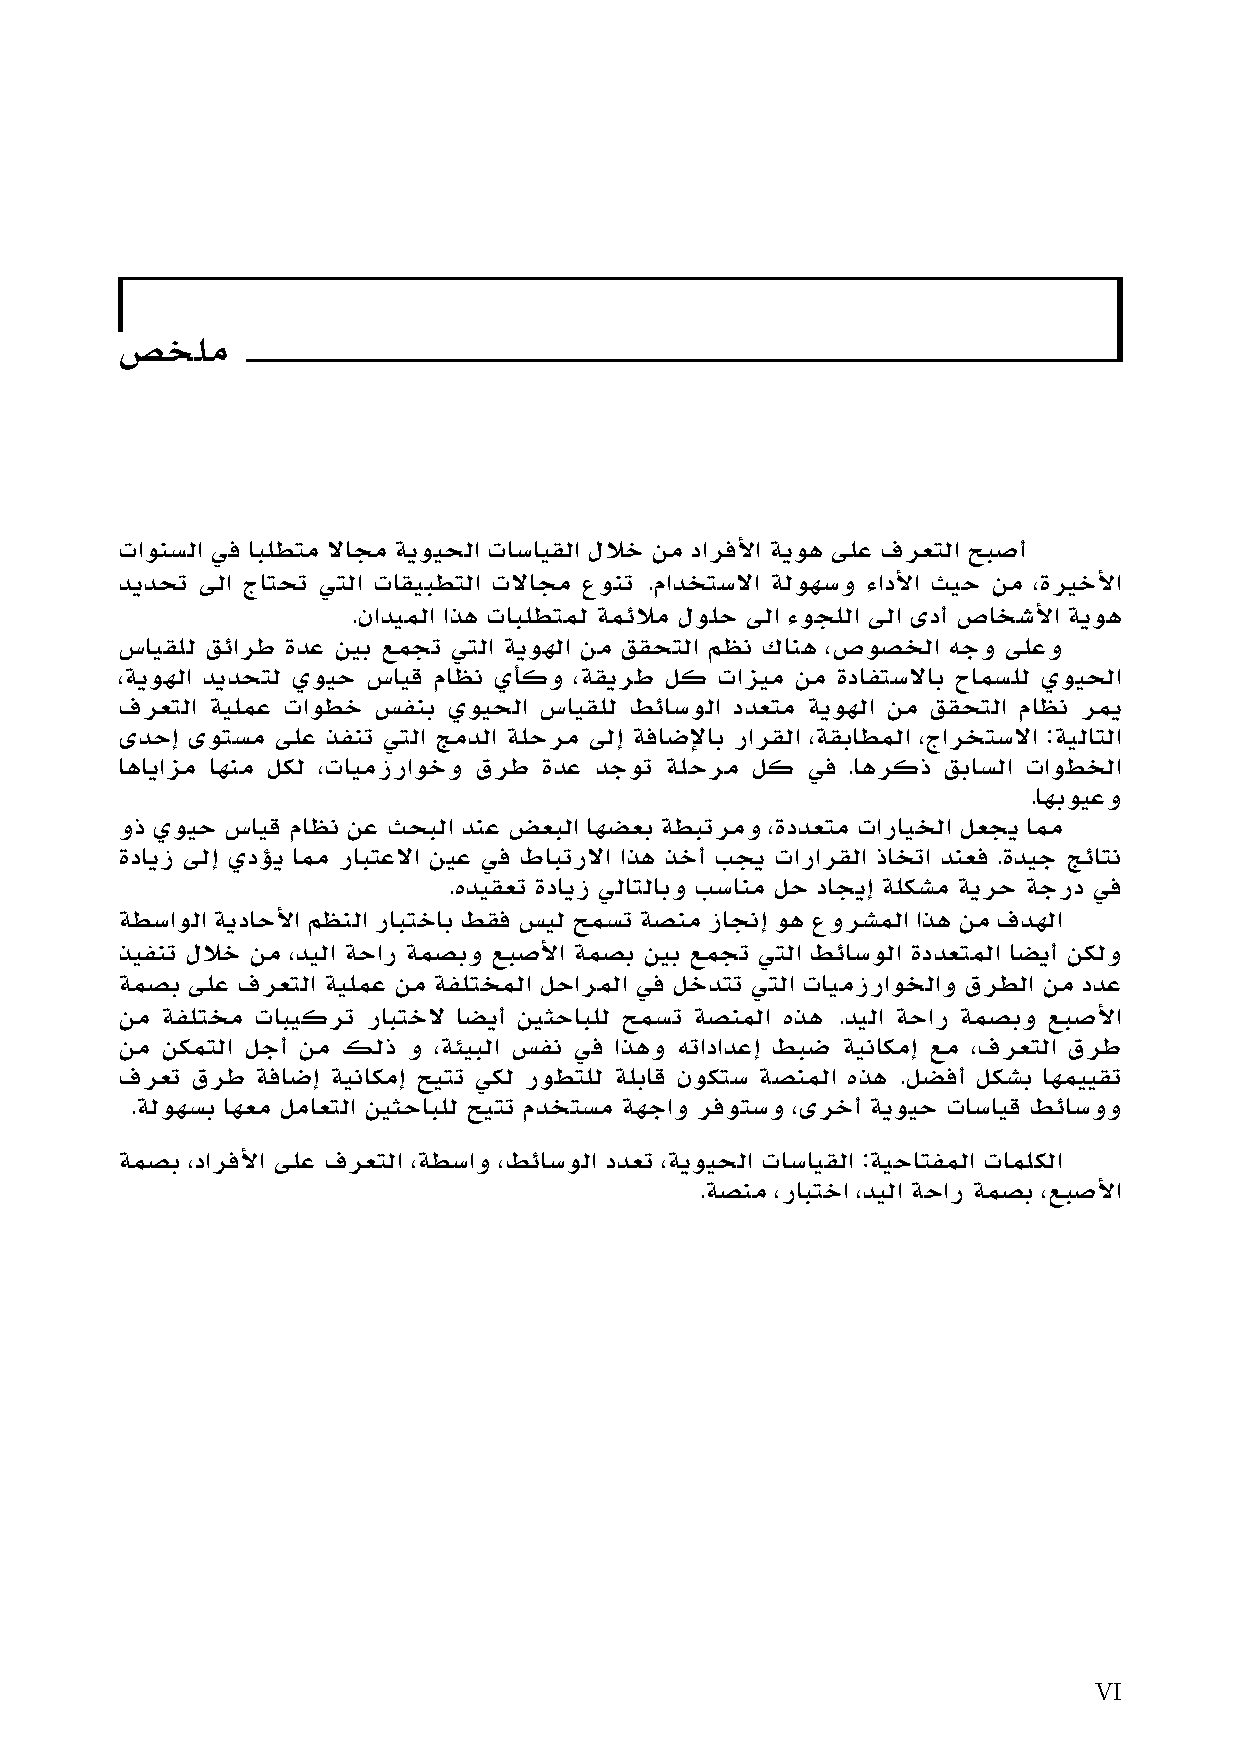
\includepdf{molakhess}
     	\pagestyle{fancy}
	\cleardoublepage
	\addcontentsline{toc}{chapter}{\contentsname}
	\tableofcontents
	\cleardoublepage
	\addcontentsline{toc}{chapter}{\listfigurename}
	\listoffigures
	\cleardoublepage
	\addcontentsline{toc}{chapter}{\listtablename}
	\listoftables
 
	
    \newpage
	\addcontentsline{toc}{chapter}{Liste des sigles et abréviations}
	\chapter*{Liste des sigles et abréviations}% Main chapter title
\begin{table}[H]
	\label{my-label}
	\begin{tabular}{ll}
	    \textbf{ACI}  & Analyse en Composantes Indépendantes     \\
	    \textbf{ACP}  & Analyse en Composantes Principales     \\
	     \textbf{ACP à noyaux}  & Analyse en Composantes Principales à noyaux     \\
	    \textbf{ACP2D}  & Analyse en Composantes Principales en deux dimensions     \\
	    \textbf{ADL}  & Analyse Discriminante Linéaire     \\
	    \textbf{BDD}  & Base De Données    \\
		\textbf{CN}   & Crossing Number                          \\
	  \textbf{DCT}  & Discrete Cosine transform                 \\
		\textbf{DET}  & Detection Error Tradeoff                 \\
		\textbf{EER}  & Equal Error Rate                         \\
     	\textbf{FMR}  & False Match Rate                     \\
		\textbf{FNMR} & False Non-Match Rate                     \\
		\textbf{k-NN} & k- Nearest Neighbor                    \\
		\textbf{MCC}  & Minutia Cylinder-Code     \\
		\textbf{OM}   & Orientations Map                         \\
		\textbf{PIN}  & Personal Identification Number                \\
		\textbf{ROC}  & Receiver Operating Characteristic        \\
		\textbf{RoI}  & Region of Interest                       \\
		\textbf{SDK}  & Software Development Kit                 \\
	    \textbf{SIFT}  & Scale-Invariant Feature Transform                \\

		\textbf{SP}   & Singulier Points      \\       
		\textbf{SVM}  &  Machines à Vecteurs de Support     \\  
		\textbf{TR}  &  Taux de Reconnaissance                    \\  

	\end{tabular}
\end{table}
	\cleardoublepage
	\addcontentsline{toc}{chapter}{Introduction}
	% Chapter Template
\chapter*{Introduction}% Main chapter title
\lhead{INTRODUCTION}
\tab Aujourd'hui, avec l'évolution technologique et l'informatisation des différentes activités, le contrôle d'accès aux données est devenu un aspect primordial, et sa sécurisation peut être si importante que l'activité elle-même, ceci nous mène à parler de la reconnaissance des individus qui est un axe de recherche en plein développement. Ce contexte rend les méthodes traditionnelles de reconnaissance des individus insuffisantes comme le mot de passe qui peut être compromis par un tiers, ou la puce électronique qui peut être volée. Cela conduit à utiliser des moyens permettant d'identifier les individus d'une manière fiable et performante en assurant un service important de la sécurité qui est la non-répudiation. La biométrie qui est la reconnaissance des individus à partir de leurs traits physiques distinctifs, s'est imposée ces dernières années dans plusieurs applications comme l'accès aux établissements, la connexion aux réseaux informatiques, le pointage du personnel …etc., dans différents domaines comme le commerce, la médecine et le gouvernement. Plusieurs modalités biométriques comme l'empreinte digitale, l'iris, la signature, la marche, l'ADN et autres sont appliquées, et le choix de modalité s'effectue en fonction de l'application à développer et le niveau de sécurité exigé. \\ \tab
 

Néanmoins, l'utilisation d'une seule modalité souffre de plusieurs insuffisances vu qu'il n'existe pas de modalité satisfaisant toutes les caractéristiques qui qualifient une modalité parfaite comme la sensibilité des données biométriques à certains bruits différents d'une modalité à l'autre, la non-universalité, la sensibilité aux attaques . Le recours à d'autres alternatives devient donc nécessaire. La biométrie multimodale, une forme de la multi-biométrie combinant plusieurs modalités, est une solution permettant de bénéficier des points forts et remédier aux insuffisances de chacune. Cela permet d'offrir des systèmes biométriques plus efficaces et plus fiables. \\ \tab
Plusieurs chercheurs se sont intéressés aux multitudes de modalités et de formes biométriques. Par conséquent, plusieurs méthodes et algorithmes intervenant dans les différentes étapes du processus de reconnaissance, ont apparu. Pour obtenir et étudier l'utilité et l'efficacité d'une méthode, les chercheurs ont besoin de les tester soit par eux-mêmes ou bien en les envoyant à des plateformes dédiées aux tests des méthodes biométriques selon la disponibilité de ces dernières. Cependant, le chercheur perd beaucoup de temps et d'effort pendant l'implémentation du test et s'il opte pour le test à distance, il doit attendre pour qu'il reçoit les résultats. De plus, la comparaison des résultats obtenus à partir de plusieurs plateformes, restant comme des boites noires, devient biaisée vu que ces dernières peuvent ne pas préciser le protocole de test suivi, ou ne pas correspondre aux tests effectués par le chercheur de manière autonome et différente.  \\ \tab

L'objectif de notre projet open source « Jupiter » est de concevoir et de réaliser une plateforme de test des systèmes biométriques multimodaux, qui permet le test des systèmes unimodaux et leur fusion afin de donner un système multimodal. Notre étude s'intéresse plus précisément aux méthodes de reconnaissance de deux modalités qui sont l'empreinte digitale, l'empreinte palmaire et leur fusion, avec la possibilité d'étendre la plateforme vers d'autres modalités. La plateforme contient à la base un ensemble de méthodes prêtes à tester et permet aux chercheurs d'ajouter d'autres méthodes d'empreinte digitale, d'empreinte palmaire ou de leur fusion. \\ \tab

Ce mémoire est organisé en sept chapitres répartis sur deux parties, la première partie avec ses trois chapitres constituent notre état de l'art, où le premier chapitre abordera les généralités en biométrie, la multi-biométrie et la multimodalité, le deuxième chapitre étudie la reconnaissance d'empreinte digitale et ses principales méthodes, le troisième chapitre présente la reconnaissance d'empreinte palmaire et ses principales méthodes. Nous enchaînons avec la deuxième partie qui présente notre contribution, cette partie englobe quatre chapitres. Le premier chapitre présente le contexte de projet et expose l'analyse de besoins, le deuxième chapitre montre la conception de Jupiter. Ensuite, le troisième chapitre comporte une présentation de la plateforme, les choix technologiques et les méthodes implémentées et le dernier chapitre les résultats de tests effectués. Enfin, nous clôturons ce rapport avec une conclusion et des perspectives du travail.

	\cleardoublepage
	\pagenumbering{arabic}
 
 \part{Synthèse bibliographique}
\label{part1}
\lhead{GENERALITES SUR LA BIOMETRIE}
%\epigraph{I recall seeing a package to make quotes}{Snowball}
\chapter{Généralités sur la biométrie}
\label{Chapter1} % Change X to a consecutive number; for referencing this chapter elsewhere, use \ref{ChapterX}

\section{Introduction}
\tab Les méthodes traditionnelles utilisées pour authentifier un individu se basaient sur une connaissance « knowledge-based » (exemple : les mots de passe) ou sur une possession « token-based » (exemple : les badges, la pièce d'identité, les clés, etc.). Cependant, ces deux méthodes ont leurs inconvénients, tels que le risque d'oublier le mot de passe ou être deviné par tiers ou encore perdre le badge.
Une alternative pratique et sécurisée pour répondre à ces problèmes est l'utilisation de la biométrie \citep{Perronnin2002} qui consiste à identifier une personne à partir de ses caractéristiques physiques, comportementales ou biologiques.
Dans ce chapitre, nous allons nous intéresser à des généralités sur la biométrie, nous allons présenter les modalités biométriques, les systèmes biométriques, les domaines d'application de la biométrie et la multi-biométrie, nous présentons la définition de la multi-biométrie, ses formes et nous détaillons sa forme multimodale.
\section{Modalités biométriques} 
Les caractéristiques biométriques par lesquelles il est possible de vérifier l’identité d’un individu sont appelées modalités biométriques. Ces modalités sont classées en trois catégories :
\begin{itemize}
	\item \textbf{Modalités physiques : }
	se basent sur la reconnaissance des différents traits physiques particuliers, qui sont permanents et uniques pour toute personne (empreinte digitale, visage, etc.).
	\item \textbf{Modalités biologiques : }
	se basent sur l’analyse des données biologiques liées à l’individu (ex : ADN, le salive, l'odeur, l'analyse du sang de différents signaux physiologiques, ainsi que la fréquence cardiaque ou EEG, etc.).
	\item \textbf{Modalités comportementales : }
	se basent sur l’analyse des comportements d’un individu (ex : la dynamique de frappe au clavier, la reconnaissance vocale, la reconnaissance dynamique des signatures, la démarche, etc.).
\end{itemize}
\vspace{1cm} 
Pratiquement, pour qu'une caractéristique humaine soit considérée comme une caractéristique biométrique il faut qu'elle satisfasse les exigences suivantes \citep{Ross} :
\begin{itemize}
	\item \textbf{Universalité : }tous les individus à identifier doivent posséder cette caractéristique.
	\item 
	\textbf{Unicité : }les caractéristiques doivent être suffisamment distinctes d'un individu de la population à un autre.
	\item 
	\textbf{Permanence : }elle doit être suffisamment invariante sur une période de temps.
	\item \textbf{Mesurabilité : }elle doit être mesurable quantitativement.
\end{itemize}
Du point de vue de système, les propriétés suivantes doivent être également prises en compte \citep{Ross} :
\begin{itemize}
	\item \textbf{Performance : }la précision de reconnaissance requise dans une application doit être réalisable en utilisant les caractéristiques.
	\item 
	\textbf{Acceptabilité : }désigne la volonté du sujet (l’individu) de présenter ses caractéristiques biométriques.
	\item 
	\textbf{Résistance aux attaques : }il s'agit de la difficulté d'utiliser des caractéristiques biométriques falsifiées (par exemple, des fausses empreintes digitales dans le cas des modalités physiologiques et de mimétisme dans le cas d'une modalités comportementales).
	
\end{itemize}
\vspace{1cm} 
Le tableau \ref{chap1:tab1} compare entre les modalités biométriques selon les propriétés citées précédemment :
\begin{longtable}{|p{2cm}|c|c|c|c|c|c|c|} 
	\hline
	\rot{{\textbf{\begin{tabular}[c]{@{}l@{}}Modalité\\ biométrique\end{tabular}}}}&
	\rot{\textbf{Universalité}}& \rot{\textbf{Unicité} }& \rot{\textbf{Permanence} }& \rot{\textbf{Mesurabilité}}& \rot{\textbf{Performance}}& \rot{\textbf{Acceptabilité} }& \rot{\textbf{\begin{tabular}[c]{@{}l@{}}Résistance aux\\ attaques\end{tabular}}} \\ \hline
	ADN&Elevée&Elevée&Elevée&Faible&Elevée&Faible&Faible \\ \hline
	Oreille&Moyenne&Moyenne&Elevée&Moyenne&Moyenne&Elevée&Moyenne \\ \hline
	Visage&Elevée&Faible&Moyenne&Elevée&Faible&Elevée&Elevée \\ \hline
	Thermo gramme du visage&Elevée&Elevée&Faible&Elevée&Moyenne&Elevée&Faible \\ \hline
	Empreinte digitale&Moyenne&Elevée&Elevée&Moyenne&Elevée&Moyenne&Moyenne \\ \hline
	Démarche&Moyenne&Faible&Faible&Elevée&Faible&Elevée&Moyenne \\ \hline
	Géométrie de la main&Moyenne&Moyenne&Moyenne&Elevée&Moyenne&Moyenne&Moyenne \\ \hline
	Veine de la main&Moyenne&Moyenne&Moyenne&Moyenne&Moyenne&Moyenne&Faible \\ \hline
	Iris&Elevée&Elevée&Elevée&Moyenne&Elevée&Faible&Faible \\ \hline
	Frappe de touche&Faible&Faible&Faible&Moyenne&Faible&Moyenne&Moyenne \\ \hline
	Odeur&Elevée&Elevée&Elevée&Faible&Faible&Moyenne&Faible \\ \hline
	Empreinte palmaire&Moyenne&Elevée&Elevée&Moyenne&Elevée&Moyenne&Moyenne \\ \hline
	Rétine&Elevée&Elevée&Moyenne&Faible&Elevée&Faible&Faible \\ \hline
	Signature&Faible&Faible&Faible&Elevée&Faible&Elevée&Elevée \\ \hline
	Voix&Moyenne&Faible&Faible&Moyenne&Faible&Elevée&Elevée \\ \hline
	
	\caption{Comparaison entre les modalités biométriques \citep{Jain2004}.}
	\label{chap1:tab1}
\end{longtable}


\clearpage
\section{Domaines d’application de la biométrie}
La biométrie peut être employée dans un grand nombre d'applications. Elle peut aider à rendre les opérations, les transactions et la vie quotidienne plus sûres et plus pratiques. Selon \citep{Jain2004}, les domaines d’applications de la biométrie peuvent être divisés en trois groupes :
\begin{itemize}
	\item \textbf{Applications commerciales : }telles que la connexion au réseau informatique, la sécurité des données électroniques, l'e-commerce, l’accès à Internet, les guichets automatiques, les cartes de crédit, le contrôle d'accès physique, la gestion des dossiers médicaux, etc.
	\item \textbf{Applications gouvernementales : }telles que les cartes d'identité nationale, les permis de conduire, la sécurité sociale, l'aide sociale, le contrôle des frontières, le contrôle des passeports, etc.
	\item \textbf{Applications médico-légales : }par exemple, l’identification des cadavres, les enquêtes criminelles, l’identification des terroristes, les tests de paternité et l’identification des enfants disparus, etc.
\end{itemize}

\section{Systèmes biométriques}

Un système biométrique est un ensemble de composants matériels et de données. Les composants matériels sont les capteurs et les programmes de comparaison, de classification et etc. Et les données sont les modèles numériques qui permettent de gérer une modalité biométrique, à partir de l’étape de capture des informations biométriques des individus jusqu'à l’étape de prise de décision lors d’une tentative d’accès \citep{wayman2005introduction}. Dans cette section, nous allons présenter les processus fonctionnels d'un système biométrique ainsi que son architecture, ensuite, les mesures de performances d'un système biométrique, enfin, nous exposons ses limitations.
\subsection{Processus fonctionnels d’un système biométrique}
Les systèmes biométriques ont trois processus fonctionnels divisés en deux phases : une phase pour enrôler les modèles des individus de la population et une autre phase de reconnaissance\citep{Ross2004a}.

\subsubsection{Phase d’enrôlement}
Pendant cette première phase, l’individu est enregistré dans le système pour la première fois. Une ou plusieurs modalités biométriques sont capturées et enregistrées dans une base de données. Les données de la base sont les données non biométriques dites biographiques, comme le nom, le numéro de la carte d’identité nationale, etc. (voir la figure \ref{fig:chapitre1enrollement}) \citep{meyer2009}.

\begin{figure}[H]
	\centering
	\includegraphics[width=0.9\linewidth]{processusfonctionnels1}
	\caption{Exemple d'enrôlement d’une empreinte digitale d'individu dans un système biométrique \citep{meyer2009}.}
	\label{fig:chapitre1enrollement}
\end{figure}
\subsubsection{Phase de reconnaissance}
La deuxième phase fonctionnelle d’un système biométrique peut être une authentification ou identification selon l’application concernée.
\begin{itemize}
	\item En mode d’authentification, le système doit répondre à une question de type : « Suis-je bien la personne que je prétends être ? ». L’utilisateur propose une identité au système et qui doit vérifier que l’identité de l’individu est bien celle proposée, il suffit donc de comparer le modèle extrait de l’identité prétendue. Si ce modèle a déjà une occurrence dans la base de données avec le modèle extrait de l’individu au moment de capture lors de la tentative d’authentification, on parle alors de correspondance 1:1 (voir la figure \ref{fig:chapitre1authentification}) \citep{Perronnin2002}.
	\\ Prenant un exemple d'un individu X qui souhaite retirer de l’argent à un distributeur de billets, en entrant son code personnel d’identification (code PIN), et en présentant une modalité biométrique. Le système acquiert alors les données biométriques et va les comparer uniquement avec le modèle enregistré correspondant à X, pour décider si X est authentique ou imposteur \citep{meyer2009}.
	\begin{figure}[H]
		\centering
		\includegraphics[width=0.9\linewidth]{processusfonctionnels3}
		\caption{Exemple d'authentification d’une empreinte digitale d'individu dans un système biométrique \citep{meyer2009}.}
		\label{fig:chapitre1authentification}
	\end{figure}
	\item En mode d’identification, le système doit deviner l’identité de l’individu qui affirme implicitement qu’il est déjà enrôlé par le système. Il répond donc à une question de type : « Qui suis- je ? ». Dans ce mode, le système compare le modèle de l’individu avec les différentes occurrences de la base de données. On parle alors de correspondance 1: N.
	Le système biométrique va trouver l’identité de la personne dont le modèle possède le degré de similitude le plus élevé avec le modèle biométrique présenté en entrée lors de la tentative d’identification. Si le plus grand score de similarité du modèle biométrique présenté en entrée avec tous les modèles de la BDD est inférieur à un seuil minimum fixé, l’individu est rejeté. Ce qui implique que l’utilisateur n’était pas une des personnes enrôlées par le système. Dans le cas contraire, la personne est acceptée \citep{Perronnin2002} (voir la figure \ref{fig:chapitre1identification}).\\
	Nous pouvons citer comme exemple, l’accès à un bâtiment sécurisé, où tous les utilisateurs autorisés à y entrer sont enrôlés par le système. Lorsqu’un individu essaye de pénétrer dans le bâtiment, il doit d’abord présenter ses données biométriques au système, et selon la résultat de l'identification de l’identité de l’utilisateur, le système lui accorde ou non le droit d’entrer \citep{meyer2009}.
	\begin{figure}[H]
		\centering
		\includegraphics[width=0.7\linewidth]{processusfonctionnels2}
		\caption{Exemple d'authentification d’une empreinte digitale d'individu dans un système biométrique \citep{meyer2009}.}
		\label{fig:chapitre1identification}
	\end{figure}
	
\end{itemize}
\subsection{Architecture des systèmes biométriques}
Les systèmes biométriques diffèrent l'un des autres en fonction du matériel de capture de l'information biométrique utilisé, des technologies exploitées et des algorithmes appliqués. 
Dans ce qui suit, nous allons décrire la structure générale d’un système biométrique indépendamment de toute modalité, de tout matériel, de toute méthode et de toute technologie, donc un système biométrique qui est générique. Ce système biométrique dit génétique se compose principalement de cinq sous-systèmes (ou modules)\citep{iso2006iec}. La figure \ref{fig:archiofbiometricsys} illustre le flux d'informations dans un système biométrique, ses composants et ses différents modes de fonctionnements.
\begin{figure}[H]
	\centering
	\includegraphics[width=1\linewidth]{archiofbiometricsys}
	\caption{Architecture du système biométrique \citep{iso2006iec}.}
	\label{fig:archiofbiometricsys}
\end{figure}
\subsubsection{Sous système de collecte de données }
Ce système se charge de l’opération d’acquisition ou de capture de l'information biométrique. Les sous-systèmes de collecte de données se différencient par :
\begin{itemize}
	\item Le type du capteur utilisé suivant la modalité biométrique du système global.
	\item Ses caractéristiques techniques.
	\item La manière de présenter le signal d’entrée. Exemple : image d’empreinte digitale ou enregistrement vocal.
	\item Le processus de conversion du signal d’entrée en une forme standard qui peut être manipulée par un ordinateur.
	\item La nécessité de coopération de l’individu ou non. Par exemple, prendre une image faciale ou scanner l’empreinte digitale.
\end{itemize}
\subsubsection{Sous système de traitement du signal 	}
Ce système traite d'abord les données biométriques capturées pour garder uniquement les données pertinentes qui peuvent distinguer les individus, il procède comme suit:
\begin{itemize}
	\item Élimine le bruit des données en sortie du sous-système précédent,qui peut étre généré à cause de la qualité du capteur et la résolution de l'image, les conditions d'éclairage et la position de capture.
	\item Applique une segmentation en utilisant un modèle prédéfini de segmentation afin de faciliter la phase de reconnaissance.
	\item Pour améliorer la qualité du modèle et optimiser sa taille de stockage, une opération d’extraction des caractéristiques est effectuée sur les données biométriques.
\end{itemize}

\subsubsection{Sous système de stockage de données}
Ce sous système sauvegarde les modèles biométriques des individus enrôlés. A la demande du sous système de comparaison(expliqué ci-dessous), il récupére un ou plusieurs modèles biométriques pendant la phase reconnaissance (authentification ou identification). Il s'occupe aussi de la mise à jour du modèle biométrique après une authentification ou identification si le nouveau modèle acquis est de meilleure qualité par rapport à celui déjà enrôlé du même individu.
Les modèles biométriques peuvent être enregistrés avec leurs données non biométriques, dans des bases de données souvent séparées logiquement ou physiquement pour des raisons de sécurité, sur des cartes intelligentes ou des dispositifs comme un ordinateur ou un téléphone mobile.
\subsubsection{Sous système de comparaison}
Ce système compare entre deux modèles biométriques en entrée, et selon la similarité entre eux, il donne en sortie : un score \footnote{Les scores indiquent la correspondance entre le modèle d’acquisition de chaque modalité biométrique composant le système avec le modèle enrôlé.} en cas d'une authentification, et un ensemble de scores au cas d'une identification.
\subsubsection{Sous système de prise de décision}
À partir de(s) score(s) trouvé(s) dans le précédant sous système et d’une politique de décision l’individu sera accepté ou considéré comme imposteur.\\
La politique de décision peut :
\begin{itemize}
\item Rejeter l’identité proclamée de tout individu dont le modèle biométrique n’a pas été acquis (enrôlé).
\item Accepter l’identité enrôlée, si le score est supérieur à un seuil prédéfini et le considérer comme imposteur dans le cas contraire.
\item Accepter les modèles biométriques dont les scores sont inférieurs à un seuil qui dépend de \citep{davida2002infrastructure} :	
\begin{list}{$\bullet$}{} 
	\item \textbf{L’individu : }il y des individus qui possèdent des caractéristiques distinctives plus que d’autres individus. C’est pour cette raison que le système utilise un seuil préfixé qui dépend de la distinctivité des caractéristiques de l’individu. Une distinctivité élevée engendre un seuil élevé et vice versa tout en tenant en compte des paramètres de la sécurité du système,un système biométrique avec un niveau de sécurité bas, peut tolérer les fausses acceptations alors le seuil fixé sera plus grand qu'un système biométrique de niveau de sécurité élevé.
	\item \textbf{La transaction : }pour une même application on peut voir plusieurs fonctionnalités à des droits d’accès différents, on peut associer à chaque droit d’accès un seuil pour contrôler plus l’accès à une opération ou à une donnée.
	\item \textbf{Le contexte : }d’autres informations peuvent être prises en considération pour fixer un seuil variant, comme les moments habituels d’accès au système, quand la dernière tentative d’accès était faite.
\end{list}
\item Donner à tous les individus un nombre fixe de tentatives possibles pour retourner un ou plusieurs scores inférieurs au seuil.
\end{itemize}

\subsection{Performances des systèmes biométriques }
\label{performance}
Il existe plusieurs métriques pour mesurer les performances d'un système biométrique. Dans cette section, nous présentons les mesures des taux d'erreur et les courbes de performance.
\subsubsection{Mesures des taux d’erreur }
Selon \citep{mansfield2002best}, les mesures des taux d’erreur sont divisées en trois groupes : les taux d’erreur de correspondance, taux d’erreur d'acquisition d'images et taux d’erreur de décision.
\begin{itemize}	
	\item \textbf{Taux d'erreur de correspondance} 
	\begin{list}{$\bullet$}{} 
		\item \textbf{Taux de fausses correspondances\footnote{Appelé en Anglais False Matching Rate (FMR).} : } c'est le taux introduit par l’algorithme de comparaison, entre la donnée biométrique acquise d'un individu et un modèle correspondant à un autre individu \citep{Jain2004}. 
		\item \textbf{Taux de fausses non-correspondances\footnote{Appelé en Anglais False Non-Matching Rate (FNMR).} : }c'est le taux introduit par l’algorithme de comparaison entre la donnée biométrique acquise d'un individu et le modèle correspondant au même individu \citep{Jain2004}.
	\end{list}
	\item \textbf{Taux d'erreur d'acquisition d'images} 
	\begin{list}{$\bullet$}{} 
		\item \textbf{Taux d'échec à acquérir : } reflète les tentatives de vérification ou d’identification pour lesquelles le système biométrique n’a pas pu acquérir l’information biométrique causé par les défauts de matériel, l'absence de l'individu, les conditions environnementales ...etc \citep{mansfield2002best}.
		\item \textbf{Taux d'échec à enrôler : }indique la proportion des individus pour lesquels la donnée biométrique n’a pas pu être générée correctement durant la phase d’enrôlement. Par exemple le cas où les personnes n’ont pas d’empreintes pour des raisons génétiques, ou des empreintes quasi-inexistantes pour des raisons médicales \citep{mansfield2002best}.
	\end{list}
	\item \textbf{Taux d'erreur de décision} 
	Les deux erreurs qui peuvent se produire pendant la phase de décision sont le rejet des utilisateurs \textit{légitimes} ou l'acceptation des \textit{imposteurs}.
	\begin{list}{$\bullet$}{} 
		\item \textbf{Taux de fausse acceptation : }pourcentage des imposteurs acceptés par erreur. Il est calculé comme suit :
		\begin{center}
			\begin{equation}\label{eq:TFA}
			TFA=\dfrac{Nombre \; de\; fausses \;acceptations\; (imposteurs\; acceptes)}{Nombre\; de\; tentatives \;d'acces\; non\; legitimes}
			\end{equation}
		\end{center}
		\item \textbf{Taux de faux rejets : }pourcentage des utilisateurs légitimes rejetés par erreur. Il est calculé comme suit :
		\begin{center}
			\begin{equation}\label{eq:TFR}
			TFR=\dfrac{Nombre\; de\; faux\; rejets \;(utilisateurs\; legitimes)}{Nombre\; de \;tentatives\; d'acces\; legitimes}
			\end{equation}
		\end{center}
		\item \textbf{Taux d'égale erreur : }concerne le point où FMR et FNMR sont égaux. Ce taux est fréquemment utilisé pour donner un aperçu sur la performance d'un système biométrique. Plus la valeur de ce taux d'erreur est faible, plus la précision du système biométrique est élevée \citep{liu2001practical} (voir figure \ref{fig:chapitre1err}). 
		\begin{center}
			\begin{figure}[H]
				\centering
				\includegraphics[width=0.75\linewidth]{eer}
				\caption{Equal Error Rate (EER).}
				\label{fig:chapitre1err}
			\end{figure}
		\end{center}
	\item \textbf{Taux de reconnaissance :} indique le nombre de comparaisons non erronés, il est calculé comme suit : 1 - la valeur de FNMR dans le seuil où nous avons trouvé le ERR.
		\item \textbf{Taux d'identification : }le taux d’identification au rang r est la proportion de transactions d’identification, par des utilisateurs enrôlés dans le système, pour lesquels l’identifiant de l’utilisateur est dans les r identifiants retournés.
		\item \textbf{Taux de fausse-positive identifications : }la probabilité de retourner une liste non vide dans l'identification des utilisateurs non enrôlés.
		\item \textbf{Taux de fausse-négative identifications : }le pourcentage d'échec d'identification d'un individu enrôlé où l’identifiant de l'individu ne figure pas dans la liste des identifiants retournée.
		
	\end{list}
	
\end{itemize}
\subsubsection{Courbes de performance }
\begin{itemize}
	\item \textbf{Courbe ROC : }représente graphiquement la relation entre le taux de vrais rejets FRR et taux de fausses acceptations FAR pour des différentes valeurs du seuil de décision \citep{egan1975signal}.\\
(voir figure \ref{fig:chapitre1roc}). 
	\begin{center}
		\begin{figure}[H]
			\centering
			\fbox{\includegraphics[width=0.5\linewidth]{roc}}
			\caption{Exemple de la courbe (ROC) \citep{Mainguet2017}.}
			\label{fig:chapitre1roc}
		\end{figure}
	\end{center}
	\item \textbf{Courbe DET: }c'est par essence une courbe ROC dont on représente directement l’évolution d’un taux d’erreur en fonction d’un autre pour la rendre plus lisible et plus exploitable. Le seuil de décision doit être ajusté en fonction de l'application ciblée : haute sécurité, basse sécurité ou compromis entre les deux (voir figure \ref{fig:chapitre1det}). 
	\begin{center}
		\begin{figure}[H]
			\centering
			\fbox{\includegraphics[width=0.5\linewidth]{det}}
			\caption{Exemple La courbe (DET) \citep{Mainguet2017}.}
			\label{fig:chapitre1det}
		\end{figure}
	\end{center}
	\item \textbf{Courbe cumulative des correspondances CMC : }représente les valeurs du rang d’identification et les probabilités d’une identification correcte inférieure ou égale à ces valeurs (voir figure \ref{fig:chapitre1cmc}). 
	\begin{center}
		\begin{figure}[H]
			\centering
			\includegraphics[width=0.6\linewidth]{cmc}
			\caption{Courbe de caractéristiques cumulatives de correspondance montrant la performance du rang 1 au rang 15 \citep{Hu2015}.}
			\label{fig:chapitre1cmc}
		\end{figure}
	\end{center}
\end{itemize}

\subsection{Limites des systèmes biométriques}
\label{section:limitation}

Bien que les systèmes biométriques offrent une solution fiable pour la reconnaissance et en pratique, ces systèmes sont utilisés dans nombreux systèmes commerciaux, Ils souffrent souvent des limitations suivantes \citep{jain2004multibiometric} :
\begin{itemize}
	\item \textbf{Bruit dans les données acquises : }introduit par le capteur pendant l’acquisition, il peut résulter d'un capteur défectueux ou mal entretenu. Par exemple, une image d'empreinte digitale avec une cicatrice, un échantillon de voix altéré par le froid ...etc.
	\item \textbf{Variation intra-classe : }variation entre les échantillons de la même modalité biométrique d’un même individu, elle peut être causée par une mauvaise interaction de l'utilisateur avec le capteur comme les changements de pose et d'expression faciale lorsque l'utilisateur se tient devant une caméra; elle augmente généralement le taux de faux rejets (FRR) de système biométrique. 
	\item \textbf{Similarité interclasse : }les caractéristiques extraites à partir de données biométriques d'individus différents peuvent être relativement similaires. Par exemple, une certaine partie de la population peut avoir une apparence faciale similaire due à des facteurs génétiques. Cela peut augmenter le taux de fausses acceptations (FAR) du système.
	\item \textbf{Non-universalité : }certains individus de population peuvent être incapables de présenter une modalité biométrique pour le système biométrique en raison d'une maladie ou d'une incapacité. 
	\item \textbf{Sensibilité aux attaques : }implique la falsification des modalités biométrique afin d'effectuer la reconnaissance. Les modalités les plus sensibles à ce genre d'attaque sont les modalités biométriques comportementales telles que la signature et la voix.
\end{itemize}
\section{Multi-biométrie}
Pour pallier aux limites des systèmes biométriques uni-modaux qu'on a déjà présentées dans la section \ref{section:limitation}, les systèmes multi-biométriques qui combinent des informations issues de multiples sources d’information sont une solution fiable pour aborder ces problèmes. En combinant plusieurs informations discriminantes, on souhaite améliorer le pouvoir de reconnaissance du système et augmenter la robustesse aux fraudes.\\
Dans ce qui suit, nous allons étudier les systèmes multi-biométriques, en commençant par présenter les différentes formes des systèmes multi-biométriques. Nous détaillerons par la suite une de ses formes à savoir « les systèmes multimodaux » en présentant ses avantages et ses différentes architectures. Enfin, nous exposerons la fusion multimodale et ses niveaux.
\subsection{Formes des systèmes multi-biométriques}

La reconnaissance dans un système multi-biométrique est effectuée à partir de multiples sources d'informations biométriques. Selon la nature de ces sources, les systèmes multi-biométriques peuvent être divisés en six formes \citep{ross2008introduction} : multi-capteur, multi-algorithme, multi-instance, multi-échantillon, multimodaux et forme hybride (voir figure \ref{fig:chapitre1sysmultibio})
\begin{center}
	\begin{figure}[H]
		\centering
		\fbox{\includegraphics[width=0.75\linewidth]{sysmultibio}}
		\caption{Formes de systèmes multi-biométriques \citep{jain2007technology}.}
		\label{fig:chapitre1sysmultibio}
	\end{figure}
\end{center}

Le tableau \ref{tab:comparaisonFormes} présente une comparaison entre les formes de systèmes multi-biométriques selon le nombre de sources d'information utilisées.
\begin{table}[H]
	\centering
	
	
	\begin{tabular}{|p{3cm}|p{3.2cm}|p{3.2cm}|p{4cm}|p{2cm}|}
		
		% header and footer information
		\hline
		
		\centering\textbf{Système multi-biométrique }
		& \centering	\textbf{Capteur}
		& \centering \textbf{Algorithme}
		& \centering \textbf{Instance} 
		& \textbf{Modalité} \\ \hline
		Multi-capteur&Toujours 2 &Généralement 1 \textbf{*}&Toujours 1 même modalité et même instance&Toujours 1\\ \hline
		Multi-algorithme&Toujours 1 &Toujours 2 &Toujours 1 &Toujours 1 \\ \hline
		Multi-instance&Généralement 1 \textbf{**}&Toujours 1 &2 instances d'une seule modalité&Toujours 1 \\ \hline
		Multi-échantillon&Toujours 1 &Toujours 1 &2 échantillons d'un seule modalité&Toujours 1 \\ \hline
		Multimodal&Généralement 2 \textbf{***}&Plusieurs&2 toujours&Plusieurs \\ \hline
	\end{tabular}
	\caption{Comparaison entre les différents formes de la multi-biométriques selon la source d'information \citep{dhamala2012multibiometric}.}	
	\label{tab:comparaisonFormes}
\end{table} 

\textbf{Exceptions : }
\begin{itemize}
	\item \textbf{* }Il est possible que deux échantillons provenant de différents capteurs soient traités en utilisant deux différents algorithmes d'extraction de caractéristiques biométriques. Puis, un algorithme d'appariement commun.
	\item \textbf{** }Dans certains cas, on peut utiliser deux capteurs capturant chacun une instance.
	\item \textbf{*** }Un système multimodal avec un seul capteur utilisé pour capturer deux modalités différentes, par exemple une image d’une résolution élevée utilisée pour extraire le visage et l'iris.
\end{itemize}
\subsubsection{Système multi capteur }
Plusieurs capteurs sont utilisés dans l'acquisition d'une seule modalité biométrique dans le but d'acquérir des informations complémentaires pour accroître les performances des systèmes uni-modaux. Comme exemple, nous pouvons citer l’utilisation d’un capteur optique et d’un autre capacitif pour l'acquisition de l’empreinte digitale.
\subsubsection{Système multi algorithme}
Ce type correspond aux systèmes qui utilisent plusieurs algorithmes pour traiter la même image acquise d'une même modalité biométrique. A titre d'exemple l'utilisation de deux algorithmes pour la reconnaissance des empreintes digitales, le premier traite les caractéristiques texturales, le seconde traite les minuties d’une empreinte digitale. 
\subsubsection{Système multi instance}
Ce type désigne les systèmes qui capturent plusieurs unités ou instances de la même modalité biométrique (les modalités qui possèdent plusieurs instances), et avec le même capteur. Par exemple le système de reconnaissance multi-instance d’iris utilise l’iris de l’œil droit ainsi que l’iris de l’œil gauche.
\subsubsection{Système multi échantillon }
Les systèmes où un seul capteur est utilisé pour capturer plusieurs copies de la même modalité biométrique, dans différentes positions et sous différents angles, pour obtenir une représentation plus complète. Par exemple, le cas de la reconnaissance du visage, plusieurs profils du visage sont capturés, tels que le profil frontal, le profil droit et gauche, afin de prendre en compte les variations de la pose faciale.
\subsubsection{Système multimodal}
Ce type de système combine différentes modalités biométriques du même individu. Par exemple les systèmes de reconnaissance qui fusionnent entre le visage et l'iris tel que le système présenté dans \citep{rattani2009robust}, ou l'empreinte digitale et l'empreinte palmaire \citep{chin2009integrating}.
\subsubsection{Système hybride}
Le terme système \textit{hybride} est utilisé pour décrire les systèmes qui intègrent un sous-ensemble des cinq systèmes présentés précédemment \citep{chang2005evaluation}. Par exemple, le système multimodale et multi-algorithme de \citep{brunelli1995person} qui comprend deux algorithmes pour la reconnaissance du locuteur et trois pour la reconnaissance du visage.

\subsection{Les systèmes multimodaux}
La multi-modalité consiste à combiner plusieurs preuves présentées par différentes modalités
biométriques, afin d’établir l’identité d’un individu, et d’obtenir des meilleures performances de
reconnaissance que les systèmes monomodaux \citep{ross2003information}.
Pour construire un système multimodal, une variété de facteurs doit être prise en compte lors de la conception d'un système biométrique multimodal \citep{Ross2004a}, on cite :
\begin{itemize}
	\item Le choix des modalités biométriques de base, on peut s'attendre à une amélioration de la performance en utilisant des modalités physiquement non corrélées (par exemple, l'empreinte digitale et l'iris) que l'utilisation des modalités corrélées (par exemple, le mouvement de la voix et des lèvres).
	\item Le niveau de fusion des informations fournies par multiple sources biométriques.
	\item La méthodologie adoptée pour intégrer l’information.
	Le compromis entre le coût supplémentaire et l’amélioration de la performance du système.
\end{itemize}
\subsubsection{Avantages et inconvénients de la multi-modalité }
Les systèmes multimodaux présentent plusieurs avantages, que nous présentons dans ce qui suit :
\begin{itemize}
	\item 	Les systèmes biométriques multimodaux sont capables de résoudre le problème de non universalité. Dans un système multimodal si un individu ne possède pas une modalité, on peut utiliser l’autre modalité comme alternative.
	\item 	Augmenter la précision en utilisant une stratégie de fusion afin de combiner la décision de chaque sous-système et arriver à une décision finale \citep{1_trader_2017}.
	\item 	Diminuer la possibilité des attaques en compliquant la tâche de la reconnaissance d’un individu. 
\end{itemize}	
\vspace{1cm} 
Cependant, les systèmes multimodaux ont, par rapport aux systèmes monomodaux, une période de développement et une complexité plus élevées, un coût supplémentaire résultant par l’ajout de nouveaux capteurs et une taille de données plus grande. Ainsi, un temps supplémentaire est nécessaire pour acquérir et traiter plusieurs modalités pendant la phase d’enrôlement et de reconnaissance. 
\subsubsection{Architecture des systèmes multimodaux}
Les systèmes multimodaux fusionnent plusieurs systèmes monomodaux, et nécessitent donc l'acquisition et le traitement de modalités différentes qui peuvent se faire successivement ou simultanément. On parle alors d’architecture \textbf{\textit{séquentielle}}, ou d'architecture \textbf{\textit{parallèle}}.
\paragraph*{Architecture séquentielle }: dans cette architecture, l'acquisition des images est faite séquentiellement dans un ordre prédéfini, la sortie d'une modalité est généralement utilisée pour réduire le nombre des identités possibles (nombre des individus identifiés) avant d’utiliser la modalité suivante \citep{hong1998integrating} (voir figure \ref{fig:chapitre1archiseq}). Cette architecture permet de réduire le temps global de la reconnaissance par rapport à l'architecture parallèle. Car la décision finale pourrait être faite avant l'acquisition de toutes les modalités. 
	
	\begin{center}
		\begin{figure}[H]
			\centering
			\fbox{\includegraphics[width=0.55\linewidth]{archiseq}}
			\caption{Architecture séquentielle d'un système multimodale \citep{ross2006information}.}
			\label{fig:chapitre1archiseq}
		\end{figure}
	\end{center}
\paragraph*{Architecture parallèle }: dans cette architecture, on utilise toutes les modalités de base qui sont acquises en parallèle (voir figure \ref{fig:chapitre1archipar}). C'est l'architecture la plus utilisée car elle améliore la performance et le temps d’acquisition \citep{hong1998integrating}. Cependant, elle est coûteuse en terme de temps de traitement.
	\begin{center}
		\begin{figure}[H]
			\centering
			\fbox{\includegraphics[width=0.55\linewidth]{archipar}}
			\caption{Architecture parallèle d'un système multimodale \citep{ross2006information}.}
			\label{fig:chapitre1archipar}
		\end{figure}
	\end{center}

Il est également possible de concevoir une architecture hiérarchique pour combiner les avantages de deux architectures précédentes où un sous-ensemble des modalités est acquis en parallèle et un autre en série. Cependant, ce type d'architecture n'a pas reçu beaucoup d'attention de la part des chercheurs \citep{ross2006information}.
\subsection{Fusion multimodale}
\label{fusionetat}
La fusion biométrique multimodale est un sujet d'actualité, elle permet de combiner les mesures de différentes modalités biométriques, pour renforcer les points forts et réduire les points faibles de différents systèmes biométriques fusionnés. Elle peut se faire à cinq niveaux différents : niveau capteur, niveau caractéristiques, niveau score, niveau décision ou niveau rang \citep{C.SandersonandK.Paliwal.2002}. 

\subsubsection{Niveau capteur}
Les données brutes capturées à partir des différents capteurs, ou plusieurs instances d'un seul capteur sont fusionnées pour construire un vecteur de caractéristiques. La fusion à ce niveau est la moins utilisée parce qu’il est possible d'avoir des données de différentes modalités incompatibles \citep{gudavalli2012multimodal}. Les captures utilisées doivent être compatibles. Par exemple, les images de visage obtenues à partir de plusieurs caméras peuvent être combinées pour former un modèle 3D du visage \citep{noore2015fusion}.
\subsubsection{Niveau caractéristiques}
\label{fusionmethodesscore}
Lorsque les vecteurs de caractéristiques sont homogènes\footnote{\textbf{Homogénéité des caractéristiques :} c'est lorsque les caractéristiques sont extraites d'une même modalité biométrique.} (exemple : plusieurs images de différentes instances d’une empreinte digitale), le vecteur de caractéristiques résultant peut être calculé par la somme pondérée des vecteurs de caractéristiques de chaque image, et si les vecteurs sont hétérogènes (exemple : deux modalités biométriques comme le visage et la géométrie de la main), ils peuvent être concaténés pour obtenir le vecteur de caractéristiques final. Néanmoins dans le cas d'incompatibilité des vecteurs de caractéristiques initiaux, la fusion n’est pas possible \citep{ross2006information}, Par exemple, les minuties d’une empreinte digitale et les coefficients de visage ("eigen-face coefficients").
\subsubsection{Niveau score }
On fusionne à ce niveau les scores donnés en sortie de la phase d’appariement de chaque modalité biométrique pour former un score unique qui est ensuite utilisé pour prendre la décision finale. Ce niveau est le plus utilisé.
\\	\textbf{Normalisation des scores : }
les scores combinés peuvent être homogènes et donc ne nécessiteraient aucun traitement, comme ils ne peuvent pas l’être. Par exemple, dans le cas de scores non homogènes : un algorithme qui donne en sortie une mesure de distance et une autre qui donne une mesure de similarité ou des scores qui suivent des différentes distributions statistiques, alors doivent d’abord être normalisés dans un domaine commun \citep{meyer2009}. Nous présentons les méthodes de normalisation les plus connues : 
\begin{itemize}
	\item \textbf{Min-Max (MM) : }cette méthode normalise les scores bruts appartenant à l’intervalle [0, 1] \citep{ross2006information}.
	\begin{center}
		\begin{equation}\label{eq:minmax}
		n =\dfrac{(s - min (S))}{(max (S)-min (S))}
		\end{equation}
	\end{center}
$ s $ : représente un score parmi l'ensemble de scores $ S $,	max (S) et min (S) définissent les points d'extrémité du domaine de définition des scores.
	\item\textbf{Z-score (ZS) : }cette méthode transforme les scores à une distribution avec une moyenne égale 0 et un écart type égale 1 \citep{ross2006information}.
	
	\begin{center}
		\begin{equation}\label{eq:ZS}
		n =\dfrac{(s - moyenne (S)) }{(std (S))}
		\end{equation}
	\end{center}
	Moyenne (S) et std (S) désignent respectivement la moyenne et le standard de déviation des scores.
	\item \textbf{Tanh (TH) : }
	cette méthode est parmi les techniques statistiques les plus solides. Elle trace les scores de 0 à 1 \citep{ross2006information}.
	\begin{center}
		
		\begin{equation}
		\label{eq:TH}
		n = \frac{1}{2}(tanh(\dfrac{0.01*(s - moyenne (S)) }{std (S)})+1)
		\end{equation}
	\end{center}
\end{itemize}

Après la normalisation, on utilise une méthode de combinaison parmi les méthodes suivantes :
\begin{itemize}
	\item \textbf{Somme Simple :} le score final est égal à la moyenne des scores de différentes méthodes d'appariement.
	\item \textbf{Somme Pondérée :} dans ce cas, nous attribuons un poids $ w $ à chaque méthode d'appariement, le calcul de poids est basé sur leur taux de erreur ERR, et le score final est égal à la somme pondérée de ces scores.	
	\item \textbf{Min-Max :} le score final est le maximum ou le minimum score parmi l'ensemble des scores.
	\item \textbf{Médian :} le score final est le médian de l'ensemble des scores.
	\item \textbf{Produit :} le score final est le produit des scores.
\end{itemize}
\subsubsection{Niveau décision}
Les décisions des différents systèmes biométriques sont fusionnées par une stratégie de décision, parmi plusieurs stratégies existantes comme la technique de vote majoritaire, ou en utilisant les opérateurs (ET, OU, Aléatoire, etc.). Cependant, la fusion à ce niveau est la moins performante, et elle est utilisée comme une alternative lorsque les autres niveaux sont inaccessibles \citep{jain2004multibiometric}. 
\subsubsection{Niveau rang }
Ce niveau de fusion est spécifique aux systèmes multi biométriques fonctionnant dans le mode d'identification, où la sortie de chaque classificateur est un sous-ensemble de correspondances possibles, triées dans un ordre décroissant de confiance. Ces sous-ensembles sont combinés pour obtenir un rang final.	

\section{Conclusion}
Nous avons présenté dans ce chapitre des généralités sur la biométrie, notamment les types de modalités biométriques, les domaines d’application, ensuite nous avons défini les systèmes biométriques ainsi que leurs diverses domaines, leurs modes de fonctionnement. Nous avons introduit la multi-biométrie, sa définition et ses formes. Et nous avons détaillé la forme qui nous intéresse le plus qu’est « la multimodalité ». C'est la combinaison de deux modalités biométriques ou plus. Elle est utilisée afin de minimiser le taux d’erreur et de bénéficier des avantages des modalités qui la composent.
\\Parmi les systèmes multimodaux, il existe des systèmes qui fusionnent l’empreinte digitale et l’empreinte palmaire qui sont les modalités biométriques les plus connues, les plus utilisées et les plus compatibles. Les processus de reconnaissances de ses modalités seront présentés en détails dans les chapitres qui suivent.



\lhead{SYSTEME BIOMETRIQUE BASE SUR L'EMPREINTE DIGITALE}
\chapter{Système biométrique basé sur l'empreinte digitale}
\label{Chapter2} % Change X to a consecutive number; for referencing this chapter elsewhere, use \ref{ChapterX}

\section{Introduction}
\tab Parmi les nombreuses modalités biométriques existantes, l'empreinte digitale (appelée aussi « dermatoglyphe ») est la plus utilisée pour la reconnaissance des personnes grâce à son unicité, son universalité, aisance de son acquisition et sa permanence \citep{maltoni2009handbook}. La figure \ref{chapitre2fingerstat} ci-dessous présente une statistique faite en \textit{2016} sur l'utilisation des modalités dans les systèmes biométriques.

\begin{figure}[H]
	\centering
	\fbox{\includegraphics[width=0.7\linewidth]{fingerstat}}
	\caption{Statistiques sur l'utilisation des modalités dans les systèmes biométriques\citep{Counter2016}.}
	\label{chapitre2fingerstat}
\end{figure}
Dans ce chapitre, nous présentons les caractéristiques de l’empreinte digitale. Nous détaillons les différentes étapes de son processus de reconnaissance et nous présentons une variété de méthodes utilisées dans chaque étape.

\section{Caractéristiques des empreintes digitales}

L'empreinte digitale se compose de motifs dessinés par les crêtes et les vallées de la peau. Les caractéristiques liées à l'empreinte digitale sont généralement catégorisées en trois niveaux \citep{hasan2013fingerprint} :
\begin{enumerate}
	
	
	\item 	\textbf{Les détails de niveau 1: }les caractéristiques globales (les points singuliers) visibles à l'œil. Il en existe deux types : les points cores \footnote{\textbf{Un core :} est le lieu de courbure maximale des lignes d'empreinte les plus internes.}, et les deltas \footnote{\textbf{Un delta :} est le lieu de divergence des lignes les plus internes, en d'autres termes un delta est proche du lieu où se séparent deux lignes.}, et sont considérés comme le centre de l'empreinte digitale, ces points sont utilisés dans l'alignement des empreintes digitales lors de la phase d'appariement (voir figure \ref{fig:chapitre2fingerprintlevel1}). 
	
	
	\begin{center}
		\begin{figure}[H]
			\centering
			\includegraphics[width=0.20\linewidth]{fingerlevel1}
			\captionsetup{justification=centering}
			\caption{Les points singuliers d'empreintes digitales.}
			\label{fig:chapitre2fingerprintlevel1}
		\end{figure}
	\end{center}
	
	
	\item \textbf{Les détails de niveau 2 : }sont les caractéristiques locales (les minuties), ils peuvent être les fins de lignes (terminaisons), les bifurcations, les lacs, les ponts et les iles. Elles sont utilisées par la plupart des systèmes automatisés de reconnaissance et peuvent être extraites de manière fiable à partir des images d'empreintes digitales avec une faible résolution (500 dpi), cette résolution est la résolution standard adoptée par le Bureau Fédéral d'Investigation dans leurs systèmes automatiques d'identification (AFIS) \citep{jain2007pores}.
	
	
	\item \textbf{Les détails de niveau 3 :} sont la forme des bords de crêtes, les crêtes immatures et le contour des arêtes, etc. (voir figure \ref{fig:chapitre2fingerprintlevel3}). Ce niveau est peu utilisé par les systèmes de reconnaissance, car les images capturées pour extraire les détails de ce niveau sont de haute résolution (plus de 1 000 dpi). 
	
	\begin{center}
		\begin{figure}[H]
			\centering
			\includegraphics[width=0.56\linewidth]{fingerlevel3}
			\caption{Les caractéristiques d'empreinte digitale du niveau 3.}
			\label{fig:chapitre2fingerprintlevel3}
		\end{figure}
	\end{center}
\end{enumerate}
\clearpage
Le processus de la reconnaissance des empreintes digitales passe par plusieurs phases, la première phase est l'acquisition d'images d'empreintes digitales, ensuite un prétraitement des images est fait afin d'améliorer leur qualité, suivi par une extraction de données utiles et enfin, après une comparaison entre le modèle en entrée au moment de la reconnaissance et le modèle déjà enrôlé une décision est prise. Pour réduire le nombre de comparaisons d'une empreinte digitale avec les empreintes digitales stockées dans une grande base de données, les images peuvent être classifiées en procédant par une méthode de classification.
\\
Il existe trois types d'approches des systèmes de reconnaissance : approches basées sur la corrélation, approches basées sur les minuties et approches basées sur les textures. 
Les approches basées sur les minuties sont les plus utilisées par les systèmes biométriques \citep{jiang2000fingerprint} car elles donnent des résultats plus précis \citep{o1998overview}, et ce sont les approches auxquelles nous nous intéressons le plus dans notre travail. 

\section{Extraction des minuties}
Une fois toutes les étapes de pré-traitement (voir annexe \ref{pretrait}) sont appliquées et l'image binarisée et squelettisée de l'empreinte digitale est obtenue, nous extrayons les minuties \citep{tisse2001systeme}. Il y a deux types de méthodes d'extraction des minuties : 
\begin{itemize}
	\item Les méthodes basées sur la binarisation (avec ou sans squelettisation).
	\item Les méthodes directes (sans passer par le prétraitement).
\end{itemize}
La majorité des systèmes de reconnaissance utilisent les méthodes basées sur la binarisation, avec une étape de squelettisation pour avoir une image de l'empreinte de qualité meilleure \citep{bansal2011minutiae}. Dans certaines méthodes d'extraction, nous procédons par une étape d'élimination des fausses minuties qu'on présente dans l'annexe \ref{posttrait}.
\subsection{Extraction avec le nombre de connexions (CN)}
\label{chp2cn}
La plupart des recherches sur la reconnaissance des empreintes digitales extraient les minuties à l'aide de la méthode du nombre de connexions CN (Crossing Number) \citep{Thai2003}.
\\
Le nombre CN d'un pixel P dans une image binarisée est calculé comme suit \citep{maltoni2009handbook} :
\begin{center}
	\begin{equation}\label{eq:cn}
	CN (P) = \frac{1}{2}\sum_{i=1}^{8}|val (P_{i mod 8 } )- val(P_{i-1}) |
	\end{equation}
\end{center}
$ P_{i} $ est la valeur du pixel voisin à celui pour lequel le CN est calculé.
\\En utilisant les propriétés du CN, chaque pixel d'une crête peut être classé comme un point intermédiaire (non-minutie), une terminaison ou une bifurcation.

\begin{center}
	\begin{figure}[H]
		\centering
		\includegraphics[width=0.6\linewidth]{cn}
		\caption{Nombre de connexions ; a). Point intermédiaire b). Terminaison ; c). Bifurcation \citep{maltoni2009handbook}.}
		\label{fig:chapitre2cn}
	\end{figure}
\end{center}

\subsection{Extraction à base morphologique}
Ces techniques d'extraction sont basées sur une morphologie mathématique dans laquelle l'image est pré-traitée, ensuite, un autre traitement avec des opérateurs morphologiques (Ouverture) et (Fermeture) est effectué, où l'opération d'ouverture est pour la suppression des pics introduits par le bruit de fond et l'opération de fermeture pour l'élimination de petites cavités, et enfin, les minuties sont extraites à l'aide de la transformation morphologique en tout ou rien « hit or miss transformation », la technique développe une structure pour chaque type de minutie, par exemple les terminaisons de crête sont les pixels d'une image qui n'ont qu'un voisin dans un voisinage de $ 3 * 3 $. Des exemples d'utilisation de cette technique dans \citep{humbe2007mathematical} et \citep{bansal2010effective}.


\section{Appariement}
L'appariement des empreintes digitales est une étape cruciale dans les problèmes d'authentification et d'identification, elle consiste à comparer entre deux empreintes digitales et retourne un degré de similarité (un nombre réel appartient à un intervalle) ou décision binaire (accepté ou non-accepté). Il existe deux grandes approches pour l'appariement des minuties : une approche globale et une approche locale \citep{maltoni2009handbook}.

\subsection{Formulation du problème d'appariement}
Nous représentons dans ce qui suit le modèle enrôlé d'une empreinte digitale par $ (T) $ et le modèle en entrée par $ (E) $, et chaque élément du vecteur de caractéristiques (vecteur de minuties) en sortie par $ (M) $, un élément du vecteur (minutie) est désigné par : 
\begin{itemize}
	\item son type (terminaison ou bifurcation);
	\item ses coordonnées cartésiennes $ (x, y) $;
	\item son orientation ($\theta$).
\end{itemize}
	$ (T) $ et $ (E) $ sont représentés par les équations \ref{eq:t} et \ref{eq:e} respectivement : 
\begin{center}
	\begin{equation}\label{eq:t}
	\abovedisplayskip
	\belowdisplayskip
	T=(M_{1},M_{2}, ..., M_{n})\qquad M_{i}=(x_{i},y_{i},\theta_{i})\quad i = 1 .. n
	\end{equation}
\end{center}

\begin{center}
	\begin{equation}\label{eq:e}
	E=(M\prime_{1},M\prime_{2}, ..., M\prime_{n\prime})\qquad M\prime _{i\prime }=(x\prime _{j },y\prime_{j},\theta\prime_{j}) \quad j = 1 .. n\prime
	\end{equation}
\end{center}
\clearpage
La représentation graphique d'une minutie est illustrée dans la figure \ref{fig:chapitre2minutiarepresentation}.
\begin{center}
	\begin{figure}[H]
		\centering
		\includegraphics[width=1\linewidth]{minutiarepresentation}
		\captionsetup{justification=centering}
		\caption{Représentation basique des minuties a) une terminaison, b) une bifurcation \citep{maltoni2009handbook}.}
		\label{fig:chapitre2minutiarepresentation}
	\end{figure}
\end{center}
Une minutie $ M_{j} $ dans $ T $ et une minutie $ M_{i} $ dans $ E $ sont considérées appariées, si $ M_{j} $ tombe dans la zone de tolérance de $ M_{i} $. Une zone de tolérance est définie par une distance spatiale ($ sd $) maximale et une différence directionnelle ($ dd $) afin de compenser les erreurs inévitables faites lors de la phase d'extraction des minuties ou par les changements de positionnement produits par des distorsions dans l'empreinte digitale (voir les équations \ref{eq:sd} et \ref{eq:dd}). Pour maximiser le nombre de minuties de $ E $ qui correspondent à $ T $ le modèle enrôlé, il nous faut un alignement de deux modèles (cela inclut également le déplacement, la rotation et d'autres transformations géométriques), après cet alignement, un score de similarité entre les deux modèles est calculé.

\begin{center}
	\begin{equation}	
	\label{eq:sd}	
	sd(M_{i},M\prime_{j})=\sqrt{(x_{i}-x\prime _{j})^{2}+(y_{i}-y\prime _{j})^{2}} \; \leq r_{0}
	\end{equation}
\end{center}
\begin{center}
	\begin{equation}\label{eq:dd}	
	dd(M_{i},M'_{j})=\min(\mid\theta_{i}-\theta \prime _{j}\mid, 360^{o} - \mid\theta_{i}-\theta \prime _{j}\mid) \; \leq \theta_{0}
	\end{equation}
\end{center}
Le score de similarité est souvent calculé par l'équation suivante \citep{maltoni2009handbook} :
\begin{center}
	\begin{equation}\label{eq:ss}	
	Score\;de\; similarite=\dfrac{k}{\dfrac{n+n \prime}{2}}
	\end{equation}
\end{center}
\textbf{$ k : $} représente le nombre de minuties appariées, $ n $ le nombre de minuties dans $ T $ et $ n \prime $ le nombre de minuties dans $ E $. 

\subsection{Approches globales }
L'alignement dans ces approches est une étape obligatoire afin de maximiser le nombre de minuties appariées, il est exécuté en prenant en considération toutes les minuties dans leur ensemble global, par le calcul de paramètres de transformation : déplacement (en $ x $ et $ y $), rotation ($ \theta $) et d'autres informations comme le changement d'échelle (dans le cas où les deux empreintes sont acquises par des capteurs de résolutions différentes). \\
La figure \ref{fig:alignement} représente les étapes de l'appariement global : 
\begin{center}
	\begin{figure}[H]
		\centering
		\includegraphics[width=0.55\linewidth]{alignement}
		\caption{Processus générique d'un appariement global \citep{Jianjiang2010Finger}.}
		\label{fig:alignement}
	\end{figure}
\end{center}

Après l'enrôlement de chaque modèle, certaines approches globales passent par une phase de pré-alignement qui est basée sur d'autres caractéristiques extraites telles que les points singuliers ou la carte d'orientation. Ces caractéristiques seront sauvegardées dans la base de données avec le modèle. Dans le suivant, nous présentons quelque approches globales. 
\subsubsection{Approche basée sur la transformée de Hough}
\label{chp2hough}
\citep{ratha1996real} ont proposé une approche d'appariement basée sur la transformée généralisée de Hough (voir annexe \ref{Hough}), dont la transformation d'alignement est estimée en discrétisant l'espace de recherche. Selon Mr. Maltoni, cette approche est la plus représentative de l'appariement global \citep{maltoni2009handbook}.

\subsubsection{Approche basée sur la géométrie algébrique}
C'est une approche plus simple que l'approche précédente \citep{maltoni2009handbook}, elle était introduite par \citep{udupa2001fast} qui ont considérablement amélioré une idée précédemment publiée par \citep{weber1992cost}, les changements d'échelle qui sont des transformations rigides ne sont pas autorisés dans cette approche. 
\subsubsection{Approche basée sur le pré-alignement absolu}
Un pré-alignement est opéré sur chaque image de la base de données indépendamment d'autres images avant d'être stockées. La méthode de M82 du FBI est la méthode la plus populaire de cette approche, elle effectue un pré-alignement absolu en fonction de la position du core détectée par la méthode R92 \footnote{Rule-based (R92) : une méthode basée sur les règles utilisée pour détecter le core de l’empreinte digitale en exploitant la carte d’orientation.}.

\subsubsection{Approche basée sur le pré-alignement relatif}
Le pré-alignement sur chaque image dépend des autres images de la base de données. Cette approche est plus robuste que l'approche absolue, mais moins rapide, le pré-alignement peut être effectué de plusieurs manières :
\begin{itemize}
	\item en superposant les points singuliers après la détection de la position du point singulier central (core ou delta);
	\item en corrélant les images d'orientation par le calcul de la similarité entre la carte d'orientation (voir annexe \ref{carteOM}) de chaque image avec toute transformation possible des cartes d'orientation des autres images;
	\item en comparant les caractéristiques des crêtes (par exemple, la longueur et l'orientation des crêtes).
\end{itemize}
\subsubsection{Autres approches globales d'appariement}
Il existent d'autres approches basées sur l'appariement global des minuties dans la littérature comme l'approche basée sur la modélisation de Warping \citep{meenen2006utilization}, \citep{liang2006fingerprint} et \citep{shi2009minucode}, et l'approche basée sur les algorithmes évolutifs \citep{sheng2009consensus}, \citep{sheng2007memetic} et \citep{tan2006fingerprint}, et d'autres approches expliquées dans le livre « \textit{Guide de la reconnaissance d'empreintes digitales} \citep{maltoni2009handbook}».
\subsection{Approches locales }
Malgré que l'approche globale conduit vers une distinctivité plus élevée car elle prend en considération les relations spatiales entre les minuties sur le plan global, les approches locales sont plus simples et possèdent une faible complexité de calcul et une tolérance à la distorsion vu qu'elles nous permettent d'apparier deux minuties même avec des informations partielles, car elles consistent à comparer deux empreintes digitales selon les structures locales des minuties. Ces structures se caractérisent par des propriétés invariantes par rapport à la transformation globale, telles que les déplacements et les rotations.
\\ Pour obtenir les avantages des deux types d'approches, on utilise des stratégies \textit{\textbf{hybrides}} qui effectuent un appariement des structures locales suivi d'une étape de consolidation. La première étape détermine les paires de minuties qui correspondent localement, et extrait un sous-ensemble d'alignements candidats pour $ (T) $ et $ (E) $, et la deuxième étape, vise à vérifier dans quelle mesure les correspondances locales détiennent au niveau global. 

Les techniques d'appariement locales qui existent dans la littérature se différencient entre elles dans la topologie de la structure locale utilisée, le type de consolidation, l'utilisation des caractéristiques supplémentaires, l'utilisation de particularités des minuties et l'apprentissage des paramètres \citep{Peralta2015a} :
\subsubsection{Topologie de la structure locale }
\label{structures}
L'appariement local est basé sur le calcul de la similarité entre les régions locales de $ T $ et $ E $, dans le but d'obtenir l'invariance souhaitée en ce qui concerne les déplacements et les rotations. Ces régions sont associées à des sous-ensembles de minuties qui sont classées en structures locales et ils peuvent être construits sous différentes manières dont :
\begin{itemize}
	\item \textbf{Les plus proches voisins :} la structure locale est formée par une minutie centrale et un certain nombre prédéterminé de ses plus proches minuties, ce type de structure est généralement défini par une distance, une direction et un angle entre les paires de minuties \citep{jiang2000fingerprint}.
	\item \textbf{Le rayon fixe :} la structure locale est créée à partir d'une minutie centrale et ses voisins dans une courbe de rayon R \citep{ratha2000robust}.
	\item \textbf{La texture mixte :} la structure locale est définie comme un vecteur de caractéristiques qui contient des informations appropriées extraites de la minutie et d'autres types d'informations provenant d'autres caractéristiques extraites de l'image d'empreinte, telles que l'orientation locale, la fréquence des crêtes, la représentation d'image en niveau de gris ou autres \citep{benhammadi2007fingerprint}.
	\item \textbf{Les triplets des minuties : }cette méthode de structuration est appelée aussi les triangles des minuties, les triplets sont construits sous forme de triangulation, en suite pour former les structures locales on utilise des informations extraites à partir de ces triangles comme les angles des sommets, la longueur des côtés et certaines propriétés du triangle telles que la direction et l'orientation \citep{maltoni2009handbook}.
	\item \textbf{K-Plet :} c'est une dérivation de la structure locale « plus proches voisins » présentée par \citep{chikkerur2006k}, où les voisins les plus proches sont également répartis dans les quatre quadrants autour de la minutie centrale.
	\item \textbf{Le cylindre de minutie :} une extension de la structure locale à rayon fixe, elle permet d'encoder les relations spatiales et directionnelles pour chaque minutie afin de rendre le calcul de la similarité des structures locales plus simple \citep{cappelli2010minutia}.
	\\
	La figure \ref{fig:chapitre2localTypes} illustre les différentes structures locales précédemment présentées.
	
	\begin{figure}[H]
		\centering
		\includegraphics[width=0.9\linewidth]{localTypes}
		\caption{Types des structures locales.}
		\label{fig:chapitre2localTypes}
	\end{figure}
\end{itemize}	
\subsubsection{Consolidation}
Bien que, à partir des scores partiels de la comparaison des structures locales nous pouvons avoir un score final, mais généralement, on procède par une phase supplémentaire pour vérifier si l'appariement local de deux minuties correspond au niveau global \citep{maltoni2009handbook}. Parmi les différentes techniques de consolidation qui ont été proposées :
\begin{itemize}
	\item \textbf{La transformation unique :} basée sur l'alignement des minuties centrales de T et E en utilisant la meilleure transformation (le déplacement et la rotation) provenue de minuties qui possèdent le meilleur score d'appariement local \citep{jiang2000fingerprint}.
	\item \textbf{La transformation multiple :} plusieurs transformations sont effectuées dans l'alignement des deux structures locales, ce type de transformation est employé dans le cas d'une empreinte digitale de mauvaise qualité ou une empreinte déformée \citep{maltoni2009handbook}.
	\item \textbf{Le consensus des transformations : }consiste à trouver le nombre maximal de transformations cohérentes pour chaque structure locale \citep{maltoni2009handbook}.
	\item \textbf{La consolidation incrémentale :} ce type est compatible seulement avec les structures locales arrangées sous forme des graphes orientés où les K-plets sont les nœuds. L'appariement est effectué en parcourant les graphes en largeur et enfin le nombre des nœuds appariés est retourné, ce processus est répété pour chaque paire de minutie et la paire ayant le meilleur score est choisie \citep{chikkerur2006k}.
\end{itemize}
\subsubsection{Utilisation des caractéristiques supplémentaires}
Dans certaines méthodes d'appariement, il est possible d'utiliser des caractéristiques supplémentaires recueillies auprès d'autres sources comme les informations extraites à partir de l'image d'orientation locale ou l'estimation locale de fréquence de crêtes \citep{Peralta2015a}. Les caractéristiques supplémentaires qui peuvent être utilisées sont les suivantes :
\begin{itemize}
	\item \textbf{La fréquence des crêtes : }représente la distance moyenne locale entre les crêtes sur un bloc et peut être utilisée comme une caractéristique locale associée aux minuties, quand elle est relativisée par rapport à la fréquence des crêtes globales ou pour normaliser les distances entre deux minuties \citep{chikkerur2007fingerprint}.
	\item \textbf{Les points singuliers :} les positions et les orientations des points singuliers peuvent être utilisées dans l'appariement local, comme notamment dans l'article \citep{zhang2002core} et \citep{feng2008combining}.
	\item \textbf{L'orientation locale des crêtes :} l'image est divisée en blocs qui ne se chevauchent pas et une valeur d'orientation est calculée à partir l'orientation de chaque pixel composant le bloc. La valeur d'orientation du bloc peut être associée à la minutie centrale d'une structure locale \citep{maltoni2009handbook}. 
	\item \textbf{L'image en niveau de gris :} elle inclut des informations sur la texture telles que les régions d'image d'empreinte améliorée par des filtres \citep{Peralta2015a}.
\end{itemize}
\subsubsection{Particularités dans les minuties}
Ce sont les informations complémentaires étroitement liées à la minutie. Les plus importantes sont :
\begin{itemize}
	\item \textbf{Types de minutie :} il existe plusieurs types. Les plus utilisés sont les \textit{\textbf{bifurcations}} et les \textit{\textbf{terminaisons}}. Car les autres types de minuties ne sont que des résultats de combinaisons de ceux-ci. Par exemple, les iles peuvent être visualisées en tant que deux bifurcations (voir Figure \ref{fig:chapitre2types}). 
	\begin{center}
		\begin{figure}[H]
			\centering
			\fbox{\includegraphics[width=0.55\linewidth]{chapitre2types}}
			\caption{Différents types de minuties : (a)terminaison (b) bifurcation, (c) pont, (d) lac et (e) ile.}
			\label{fig:chapitre2types}
		\end{figure}
	\end{center}
	\item\textbf{Nombre de crêtes :} représente le nombre de crêtes associées à chaque minutie centrale de la structure locale.
	\item \textbf{Propriétés des crêtes :} comme le rayon de courbure de crête à laquelle la minutie appartient.
\end{itemize}
\subsubsection{Apprentissage de paramètres }
Des techniques d'apprentissage qui se basent sur les machines learning sont généralement employées dans l'optimisation du score de similarité qui détermine la décision finale. Les formes d'apprentissage des paramètres sont les suivantes :
\begin{itemize}
	\item \textbf{Score de similarité :} une fonction qui reçoit les vecteurs de caractéristique représentant deux structures locales de $ E $ et $ T $ et donne comme résultat le score de similarité optimisé qui est appris à l'aide des réseaux de neurones ou d'autres schémas de régression.
	\item \textbf{Similitude locale :} un processus d'apprentissage hors ligne est effectué pour apprendre la vraie similitude entre les structures locales ou pour ajuster les poids de contribution associés à chaque élément du vecteur de caractéristiques.	
\end{itemize}
\subsubsection{Synthèse des travaux sur l'appariement local basé sur les minuties}
Dans la littérature, plus de 80 méthodes d'appariement local basées sur des minuties ont été proposées \citep{Peralta2015a}.
Le tableau \ref{tab:chapitre2fingermatching} résume quelques travaux de recherche.

\begin{sidewaystable}[h!]
	\centering
	
	\begin{tabular}{|p{4cm}|p{4cm}|p{4cm}|p{3cm}|p{3cm}|p{4cm}|}
		\hline
		\begin{center}
			\textbf{Topologie de la structure locale}
		\end{center} &\begin{center}
			\textbf{Le type de consolidation}
		\end{center} &\begin{center}
			\textbf{Caractéristiques supplémentaires utilisés}
		\end{center} & \begin{center}
			\textbf{Les particularités dans les minuties} 
		\end{center}& \begin{center}
			\textbf{La forme d'apprentissage des paramètres}
		\end{center} &\begin{center}
			\textbf{La référence}\begin{center}
				
			\end{center}
		\end{center} \\ \hline
		La texture mixte & Transformation unique & 
		L'orientation locale des crêtes
		& Types de minutie et Propriétés des crêtes & Aucune & \citep{he2003image} \\ \hline
		K-Plet & Incrémentale & Les points singuliers & Types de minutie & Aucune & \citep{chikkerur2005impact} \\ \hline
		La texture mixte et les triplets des minuties & Le consensus des transformations & L'orientation locale des crêtes & Aucune & Similitude locale & \citep{chen2006algorithm} \\ \hline
		La texture mixte & Transformation multiple & L'image en niveau de gris & Aucune & Aucune & \citep{benhammadi2007fingerprint} \\ \hline
		Les plus proches voisins & Incrémentale & Aucune & Aucune & Aucune & \citep{Watson2010} \\ \hline
		Le rayon fixe et la texture mixte & Transformation multiple & La fréquence des crêtes et l'orientation locale des crêtes & Propriétés des crêtes & Score de similarité & \citep{cao2009fingerprint} \\ \hline
		Les plus proches voisins & Transformation unique & Aucune & Les types de minutie et le nombre de crêtes & Aucune & \citep{jiang2000fingerprint} et \citep{bengueddoudj2013improving} \\ \hline
		La texture mixte et les triplets des minuties & Aucun & L'image en niveau de gris et les points singuliers & Aucune & Aucune & \citep{mistry2013fusion} \\ \hline
	\end{tabular}
	\caption{Quelques travaux de recherche sur l'appariement local basé sur les minuties.}% Add 'table' caption	
	\label{tab:chapitre2fingermatching}	
\end{sidewaystable}
\clearpage
\section{Classification des empreintes digitales}
\label{fingerprintclassification}
La classification des empreintes digitales est une technique efficace qui permet de réduire le nombre de comparaisons d'une empreinte digitale avec les empreintes digitales stockées dans une grande base de données, par conséquent cela va permettre de réduire le temps de recherche.
\\ Le principe est de partitionner la base de données en plusieurs classes en utilisant des caractéristiques extraites de l'empreinte digitale (par exemple : le nombre et la position de points singuliers, les orientations, les réponses aux filtres de Gabor, etc.), ensuite attribuer chaque empreinte digitale enrôlée à une classe. \\
Les approches de classification existantes peuvent être attribuées à l'une des catégories suivantes : les approches syntaxiques, les approches structurales, les approches statistiques, les approches neuronales, les approches qui utilisent les SVM. Ces approches sont soit des approches fixes ou basées sur des techniques d'apprentissage, nous les présentons dans ce qui suit :
\subsection{Système de classification de Henry}
Les premières recherches scientifiques sur la classification des empreintes digitales ont été faites par \citep{galton1892finger}, qui a divisé les empreintes digitales en trois grandes classes. Plus tard, Henry et Edward Richard ont redéfini la classification de Galton en augmentant le nombre des classes à cinq \citep{henry1905classification} : la boucle droite (Right Loop (R)), la boucle gauche (Left Loop (L)), la volute (Whorl (W)), l'arche (Arch (A)) et l'arche lentiforme (Tented Arch (T))(Edward Richard, 1900), ces classes d'empreintes digitales sont inégalement réparties dans la population (3,7\%, 2,9\%, 31,7\%, 33,8\% et 27,9\%, respectivement \citep{peralta2017robust}). 
\\ Un exemple pour chaque classe sont présentés dans la figure \ref{fig:chapitre2henryclasses}. 
\begin{figure}[H]
	\centering
	\includegraphics[width=0.7\linewidth]{chapitre2henryclasses}
	\caption{Classes d'empreinte digitale : a) boucle, b) boucle droite, c) volute, d) arche, e) arche lentiforme.}
	\label{fig:chapitre2henryclasses}
\end{figure}


\subsection{Approches syntaxiques}
Ces approches sont basées sur l'extraction des symboles à partir des caractéristiques de l'empreinte. L'idée de base consiste à définir une grammaire pour chaque classe d'empreinte digitale, ensuite la classification est effectuée par une analyse syntaxique afin de déterminer quelle grammaire génère les symboles extraits\citep{mridula2014review}. La figure \ref{fig:chapitre2classificationsyntax} illustre une méthode introduite par Rao et Balck 1980 qui se base sur l'analyse des flux de lignes de crêtes \citep{karu1996fingerprint}.


\begin{center}
	\begin{figure}[H]
		\centering
		\fbox{\includegraphics[width=0.55\linewidth]{chapitre2classificationsyntax}}
		\caption{Un schéma de la méthode de Rao et Balck \citep{karu1996fingerprint}.}
		\label{fig:chapitre2classificationsyntax}
	\end{figure}
\end{center}
\subsection{Approches structurales}
Ce sont les approches qui se basent sur l'organisation relationnelle des caractéristiques qui est représentée par des structures de données symboliques, telles que les arbres et les graphes, qui permettent d'avoir une organisation hiérarchique de l'information \citep{maio1996structural}. Exemples de ces organisations : les arbres de décision ($ DT $ Decision Trees) et les modèles de Markov cachés ($ HMM $ Hidden Markov Model).
\subsection{Approches statistiques}
\label{KNN}
Dans cette approche, nous extrayons un vecteur de caractéristiques numérique de taille fixe à partir d'une empreinte digitale en se basant sur le champ d'orientation ou sur la réponse aux filtres de Gabor, nous utilisons un classificateur statistique pour la classification, parmi les classificateurs les plus utilisés, nous avons le plus proche voisin (($ k-NN $) $ k $- nearest neighbor) qui est une méthode d'apprentissage supervisée où une nouvelle empreinte digitale est classifiée à la base d'un vecteur de caractéristiques construit à partir des scores attribués, pour trouver le plus proche voisin, la distance de hamming ou angulaire est calculée entre la nouvelle empreinte digitale et chaque empreinte digitale existante dans la base de test. Le résultat final est obtenu en effectuant un tri ascendant \citep{kong2009survey}.
\subsection{Approches des réseaux de neurones }
\label{NN}
Un réseau de neurones représente un modèle de calcul composé d'entités interconnectées où l'entité est un neurone, ou une succession de couches dont chacune prend ses entrées sur les sorties de la précédente. Un neurone est caractérisé par un état d'excitation qui dépend de celui des neurones situés à la couche supérieure ainsi que de la force des liens qui les relient. Dans la majorité des cas, les neurones sont en fait des fonctions calculées par un programme informatique, mais ils sont parfois réalisés sur des circuits électroniques.
\subsection{Approche des machines à vecteurs de support (SVM) }
\label{SVM}
Cette approche englobe les méthodes d'apprentissage supervisées destinées à résoudre des problèmes de discrimination et de régression \citep{honeine2007methodes}, elles reposent sur deux principes :
\begin{itemize}
	\item \textbf{Marge maximale : }on cherche à maximiser la marge entre l'hyperplan séparateur recherché et les éléments de chaque classe de l'ensemble d'apprentissage.
	\item \textbf{Fonction noyau :} qui permet de conférer un caractère non-linéaire à nombre de traitements originellement linéaires sans qu'il soit nécessaire de recourir à d'importants développements théoriques.
\end{itemize}
Le but du SVM est de trouver une séparatrice qui minimise l'erreur de classification sur l'ensemble d'apprentissage qui sera également performante en généralisation sur des données non utilisées en apprentissage. Pour cela le concept utilisé est celui de marge (d'où le nom de séparateurs à vaste marge). La marge est la distance quadratique moyenne entre la séparatrice et les éléments d'apprentissage les plus proches de celle-ci appelés vecteurs de support. Ces éléments sont appelés vecteurs de support car c'est uniquement sur ces éléments de l'ensemble d'apprentissage qu'est optimisée la séparatrice \citep{belahcene2012comparaison}.



\section{Conclusion}

Dans ce chapitre, nous avons introduit la modalité d'empreinte digitale qui est considérée comme la modalité biométrique la plus utilisée, ensuite, nous avons présenté les trois niveaux de ses caractéristiques. Nous avons aussi expliqué le processus de reconnaissance en mettant l'accent sur l'approche basée sur les minuties. Enfin, nous avons présenté les différentes méthodes d'extraction et d'appariement des minuties. 
\\Dans le chapitre suivant nous allons présenter le processus de la reconnaissance d'empreinte palmaire.

 \lhead{SYSTEME BIOMETRIQUE BASE SUR L'EMPREINTE PALMAIRE}
\chapter{Système biométrique basé sur l'empreinte palmaire }
\label{Chapter3}
\section{Introduction}
\tab La première recherche faite sur la reconnaissance d'empreintes palmaires a été introduite par \citep{shu1998automated}, afin de pallier les problèmes liés à la non visibilité d'empreintes digitales ou bien le coût élevé des appareils de capture des images de l'iris et de la rétine ou encore les faibles taux de reconnaissance des autres modalités biométriques \citep{Wassila2007}.
\\L'empreinte palmaire ou « palmprint » est cette surface très interne de la main, elle contient plusieurs traits caractéristiques tels que les lignes principales, les plis et les textures \citep{pavevsic2004personal} (Voir la figure \ref{fig:chapitre3anatomy}). Il existe plusieurs approches afin de reconnaitre les individus en utilisant leurs empreintes palmaires, celles qui utilisent des images d'empreintes palmaires de haute résolution (i.e. résolution supérieure à 500 dpi) et celles qui utilisent des images de basse résolution (résolution inférieure à 100 dpi). La reconnaissance par des approches à basse résolution est exploitée dans les applications civiles et commerciales comme le contrôle d'accès. Cependant, la reconnaissance par des approches à haute résolution convient aux applications du secteur de la justice comme la détection des criminels.

\begin{center}
	\begin{figure}[H]
		\centering
		\includegraphics[width=0.55\linewidth]{chapitre3anatomy}
		\caption{Anatomie de l'empreinte palmaire.}
		\label{fig:chapitre3anatomy}
	\end{figure}
\end{center}
\clearpage
Le tableau \ref{tab:palmcomparaison} compare entre une image de haute résolution et une autre de basse résolution d'une empreinte palmaire :
\begin{table}[H]
	\centering
	
	\begin{tabular}{|p{5cm}|p{5cm}|p{5cm}|}
		\hline
		\textbf{Approche} & \textbf{Basse résolution} & \textbf{Haute résolution} \\ \hline
		\textbf{Résolution des Images traitées} & Inférieure à 100(500) dpi & Supérieure à 500(1000) dpi \\ \hline
		\textbf{Caractéristiques pouvant être extraites} & Lignes principales, lignes secondaires & Toutes : lignes principales, lignes secondaires et lignes fines \\ \hline
		\textbf{Applications} & Les applications civiles et commerciales comme le contrôle d'accès & Applications du secteur de la justice comme la détection des criminels \\ \hline
		\textbf{Espace mémoire exploité} : applications temps réel & Plus petit & Plus grand \\ \hline
		\textbf{Processeur }: applications temps réel & Plus rapide & Plus lente \\ \hline
	\end{tabular}
	\caption{Comparaison entre une image de haute et une image de basse résolution d'une empreinte palmaire.}
	\label{tab:palmcomparaison}
\end{table}
Dans ce qui suit, nous détaillons les différents algorithmes à basse résolution qui sont les plus utilisés dans la reconnaissance de l'empreinte palmaire \citep{kong2002palmprint}, qui interviennent essentiellement dans l'étape d'extraction. Ces algorithmes se catégorisent en trois grandes approches : l'approche holistique, l'approche à base des caractéristiques locales de la paume de main et l'approche hybride.
\section{Approche holistique (globale)}
Les algorithmes appartenant à cette approche manipulent les images comme un tout, des matrices de valeurs de pixels, à traiter d'une manière globale et il n'est pas nécessaire de repérer certains points \citep{meyer2009} pour effectuer la reconnaissance. Cette approche se base sur des techniques d'analyse statistique bien connues. Elles peuvent être linéaires ou non linéaires, supervisées ou non supervisées. Dans ce qui suit nous parlerons des méthodes d'extraction et des exemples d'algorithmes suivant l'approche holistique.
\subsection{Méthodes d'analyse des sous-espaces }
\label{spacemethodes}
Le but de ces méthodes est de transformer les données de l'image d'entrée représentées dans un espace de grande dimension en une représentation dans un espace de dimension plus faible et d'extraire l'information pertinente afin de faciliter l'étape de classification. 

\subsubsection{Analyse en composantes principales (ACP)}
\label{ACP}
L’ACP est une méthode linéaire\footnote{Une méthode linéaire : s’applique sur des données qui ont une structure linaire (vecteurs, matrices …etc.).} non supervisée\footnote{Une méthode non supervisée : c’est une méthode qu’on ne sait pas les classes des données dans la phase d’apprentissage.} utilisée pour projeter les images dans un espace de données de dimension inférieure d’une manière à garder que la donnée discriminante, cette méthode exploite la liaison entre les colonnes de l’image, et minimise le nombre de colonnes, si c’est possible, pour qu’elles soient non corrélées deux à deux\citep{lu2003palmprint}. 
\\Considérant un ensemble de $ M $ images d'empreintes palmaires $ x_{1}, x_{2},…..,x_{m} $, de dimension $ N * N $.
La moyenne des $ M $ images $\mu $ est calculée par :
\begin{center}
	\begin{equation}\label{eq:chapitre3eq1}
	\mu = \frac{1}{M}\sum_{i=1}^{M}x_{i}
	\end{equation}
\end{center}
Chaque image $ {x_{i}}$ de l'ensemble diffère de l'image moyenne de : $ Q_{i}=x_{i}-\mu$.
La matrice de covariance de la matrice est de dimension $N^{2}*N^{2}$, elle est calculée comme suit :
\begin{center}
	\begin{equation}\label{eq:chapitre3eq2}
	C = \frac{1}{M}\sum_{i=1}^{M}(x_{i}-\mu)(x_{i}-\mu)^{T}=\frac{1}{M}XX^{T} \qquad tel que : \! X= [Q_{1} Q_{2}… Q_{M}]
	\end{equation}
\end{center}

C'est évident que les vecteurs propres de la matrice $C$ forment l'espace propre (matrice) qui représente la meilleure approximation de l'ensemble des images de départ en terme de l'erreur quadratique moyenne.
\\Trouver les vecteurs propres et les valeurs propres d'une image est une tache insoluble pour une image de dimension typique assez grande. La formule suivante est satisfaite pour la matrice $C$ : $Cu_{k}= \lambda_{k}u_{k}$, tels que $u_{k}$ sont les vecteurs propres de la matrice $C $ et $\lambda_{k}$ sont les valeurs propres de $C$.
En pratique le nombre $M$ des images de l'ensemble de départ est relativement petit, les vecteurs propres $(v_{k})$ et les valeurs propres$(a_{k})$ de la matrice $ L=X^{T}X(L \in\Re)$ sont beaucoup plus facile à calculer, donc nous avons : 
\begin{center}
	\begin{equation}\label{eq:chapitre3eq3}
	X^{T}Xv_{k}=a_{k}v{k} \rightarrow XX^{T}(Xv_{k})=a_{k}(Xv{k})
	\end{equation}
\end{center}
Nous obtenons par la suite les valeurs propres de $C$ $u_{k}=Xv_{k}$, tels que $ U=\begin{Bmatrix}u_{k},k=1,..,M \end{Bmatrix} $ dénote les vecteurs de bases qui correspondent aux images d'empreinte palmaire originales formant un espace propre unitaire.
\\ L'utilisation de la méthode d'analyse en composante principale nous permet de choisir les vecteurs propres correspondant aux valeurs propres les plus grandes qui permettent de mieux représenter les images d'empreinte palmaire du départ. Les $ {M}'$ vecteurs propre significatifs $({u}'_{k})$ associés aux valeurs propres les plus grandes sont sélectionnés comme composante des paumes propres (eigenpalm) $ {U}'=\begin{Bmatrix} {u}'_{k},k=1,..,{M}'\end{Bmatrix} $, donc une image d'empreinte palmaire est transformée en composantes de paume propre en appliquant la formule suivante : $f_{i}={U}'(x_{i}-\mu) \qquad tels que :\qquad (i=1,..M)$

Où le poids de la projection $f_{i}(f_{i} \in \Re ^{{M}'*1}))$ réfère au vecteur des caractéristiques de chaque personne et $ {M}'$ est la longueur de caractéristiques\citep{lu2003palmprint}.

La figure suivante \ref{fig:chapitre3eigenpalms} illustre les « eigenpalms » dérivées des images d'empreinte palmaires de test :
\begin{center}
	\begin{figure}[H]
		\centering
		\includegraphics[width=0.7\linewidth]{chapitre3eigenpalms}
		\caption{a) : les images d'empreintes palmaires de test, b) : les eigenpalms dérivées \citep{lu2003palmprint}.}
		\label{fig:chapitre3eigenpalms}
	\end{figure}
\end{center}
\subsubsection{Analyse en composantes indépendantes (ACI)}
\label{ACI}
L'analyse en composantes indépendantes traite des observations vectorielles (multivariées) afin d’en extraire des composantes linéaires qui soient « aussi indépendantes que possible » \citep{cardoso2002analyse}.
Une image d’empreinte palmaire est considérée comme un ensemble inconnu de sources d’images statistiquement indépendantes mélangées par une matrice de mixage.
L’ACI donc trouve une matrice de séparation afin de de transformer un signal mixte à un ensemble de signaux linéairement indépendants \citep{connie2003palmprint}.
La figure suivante \ref{fig:chapitre3etapesACI} illustre les étapes globales de l’application de l’analyse en composantes indépendantes pour la reconnaissante d’empreinte palmaire:
\begin{center}
	\begin{figure}[H]
		\centering
		\includegraphics[width=0.7\linewidth]{chapitre3etapesACI}
		\caption{Implémentation de l’ACI sur la reconnaissance d’empreinte palmaire.}
		\label{fig:chapitre3etapesACI}
	\end{figure}
\end{center}
Soit S, le vecteur des images sources inconnues, x le vecteur des mélanges observés.
Si A est la matrice de mixage alors le processus de mixage est décrit par :$x=A\hat{s}$.
\\
Le but de l'ACI est de trouver la matrice de séparation W telle que :
$\hat{s}=Wx$.
\\

Néanmoins, il n’y a pas de méthodes exactes pour calculer la matrice W, plutôt des méthodes itératives sont utilisées pour trouver une approximation à W de telle manière à optimiser l’estimation de $\hat{s}$.

Il existe plusieurs implémentations de ACI, parmi ces implémentations, l’algorithme InfoMax décrit dans l’article \citep{bartlett2002face}, qui est appliqué pour trouver la valeur de $\hat{s}$ d’abord, puis la valeur de X.
La figure \ref{fig:chapitre3ACPACI} représente les résultats obtenus après l’application de l’ACP et de l’ACI sur les mêmes images de test.
\begin{center}
	\begin{figure}[H]
		\centering
		\includegraphics[width=0.7\linewidth]{chapitre3ACPACI}
		\caption{a) Résultats générés après l’application de l’algorithme d’analyse en composantes principales (ACP), b) Résultats générés après l’application de l’algorithme d’analyse en composantes indépendantes (ACI).}
		\label{fig:chapitre3ACPACI}
	\end{figure}
\end{center}

\subsubsection{Analyse discriminante linéaire (ADL)}
\label{ADL}
C’est une méthode linéaire supervisée où la base d’apprentissage d’images est organisée en plusieurs classes : une classe par personne et plusieurs images par classe. L'ADL analyse les vecteurs propres de la matrice de dispersion des données, pour maximiser les variations interclasses tout en minimisant les variations intra-classes \citep{morizet2006revue}.
Supposons que nous avons $ C $ classes connues dans un espace de dimension N, le nombre de templates par la ième classe est noté par $l_{i}$, le nombre total des templates de toutes les classes est L,
$x_j^i$ est la $j^{eme}$ template de la $i^{eme}$ classe, $1\leq i\leq c,1\leq j\leq l_{i}$, $x_{i}$ est la $i^{eme}$ template, telle que $1\leq i\leq L$.
\\
Mathématiquement, l’objectif de l’ADL est de calculer la matrice rectangulaire $W\in R^{N*n}$qui maximise le critère de Fisher:
\begin{center}
	\begin{equation}\label{eq:chapitre3eq4}
	J(W)=\frac{\left | W^Ts_b W \right |}{\left | W^Ts_w W\right |}
	\end{equation}
\end{center}
Telles que $S_{b}$ et $S_{W}$ sont les matrices dispersions interclasses et intra classes, respectivement
\begin{center}
	\begin{equation}\label{eq:chapitre3eq5}
	S_b=\sum_{i=1}^{c}P_i(m_i -m)(m_i-m)^T
	\end{equation}
\end{center}
\begin{center}
	\begin{equation}\label{eq:chapitre3eq6}
	S_w=\sum_{i=1}^{c}\sum_{j=1}^{l_{i}}(x_{j}^{i}-m_{i})(x_{j}^{i}-m_{i})^{T}
	\end{equation}
\end{center}
où $m_i=\frac{1}{l_i}\sum_{j=1}^{l_i}x_{j}^{i}$, $m=\sum_{k=1}^{L}x_{k}=\sum_{i=1}^{c}p_{i}m_{i}$ Sont la moyenne des templates de la $i^{eme}$ classe et la moyenne de toutes les templates respectivement.
$W$ doit être composée des vecteurs propres correspondants aux valeurs propres de l’équation :
\begin{center}
	\begin{equation}\label{eq:chapitre3eq7}
	S_b \alpha _i=\lambda_i S_w \alpha_i
	\end{equation}
\end{center}
Si $S_{W}$ est une matrice non singulière, les $k$ vecteurs discriminants seront les $k$ vecteurs propres correspondants aux $k$ plus grandes valeurs propres de la matrice $S_{w}^{-1}S_{b}$.
\subsubsection{Analyse en composantes principales à noyaux (ACP à noyaux)}
L'un des inconvénients de l'ACP réside dans sa linéarité. Des vecteurs principaux sont obtenus indépendamment du fait que des lois non-linéaires puissent régir le comportement du système étudié (le changement de luminosité, de position) \citep{honeine2007methodes}. Dans l'analyse en composantes principales à noyaux qui est une méthode non linéaire\footnote{Une méthode non linéaire : c'est une méthode qui s'applique sur des données non linéaires (arbre par exemple), les données (non linéaires) sont transformées non linéairement par une fonction mathématique vers un espace d’une plus grande dimension où les données non linéaires peuvent être linéairement séparable \citep{diederich2001face}.}.
Étant donné un ensemble de $ m $ variables centrées $x_{k}$, $x_{k}=[x_{k1},...,x_{kn}]^{T}\in R^{n}$.
\\
Dans la méthode ACP (voir la section \ref{ACP}), l’équation: $w\lambda =Cw$ est vérifiée, telles que $\lambda \geq 0$, et les $\lambda$ sont les valeurs propres et $W\in R^{n}$ sont les vecteurs propres correspondants.
Dans la méthodes ACP à noyau, les vecteurs $ x $ sont projetés de l’espace d’entrée $R^{n}$ vers un espace de dimension plus grande $R^{f}$ par une fontion non lineaire :
\begin{center}
	\begin{equation}
	\label{eq:chapitre3eq8}
	\Phi :R^{n}\rightarrow R^{f}, f\gg n	
	\end{equation}
\end{center}
Dans $R^{f}$ trouver les valeurs propres revient à résoudre l’équation \ref{eq:chapitre3eq9} :
\begin{center}
	\begin{equation}
	\label{eq:chapitre3eq9}
	\lambda W^{\Phi }=C^{\Phi }W^{\Phi } 
	\end{equation}
\end{center}
Telle que $C^{\Phi }$ est la matrice de covariance. Les solutions $W^{\Phi }$, $\lambda \neq 0$ s’étendent vers $\Phi \left (x_{1} \right),...,\Phi \left (x_{m} \right)$ et il existe des coefficients $\alpha _{i}$ tels que 

\begin{center}
	\begin{equation}\label{eq:chapitre3eq10}
	w^{\Phi }=\sum_{i=1}^{m}\alpha_{i}\Phi \left (x_{i} \right)
	\end{equation}
\end{center}
Notons la matrice $K$ de dimension $m*m$:

\begin{center}
	\begin{equation}\label{eq:chapitre3eq11}
	K_{ij}=k(x_{i},x_{j})=\Phi (x_{i}).\Phi(x_{j})
	\end{equation}
\end{center}
Donc, le problème de l’ACP à noyau devient :
\begin{center}
	\begin{equation}\label{eq:chapitre3eq12}
	\lambda K\alpha=K^2 \alpha
	\end{equation}
\end{center}
\begin{center}
	\begin{equation}\label{eq:chapitre3eq13}
	m\lambda \alpha=K\alpha
	\end{equation}
\end{center}
Tel que $\alpha$ est le vecteur colonne qui regroupe les coefficients $\alpha _{1},...,\alpha _{m}$.
C’est possible maintenant de projeter les vecteurs de $R_{f}$ vers un espace de dimension plus petite engendré par les vecteurs propres $W^{\Phi }$.
Soit $x$ une template(une image d’empreinte palmaire) et $\Phi (x)$, sa projection dans $ R^{f} $, la projection de $\Phi (x)$ sur $W\left (\Phi \right)$ est constituée des composantes principales non linéaires correspondantes à $ \Phi $ :
\begin{center}
	\begin{equation}
	\label{eq:chapitre3eq14}
	W^{\Phi }\Phi(x)=\sum_{m=1}^{m}\alpha_{i}(\Phi(x_{i}).\Phi(x))=\sum_{m=1}^{m}\alpha_{i}k(x_1,x)
	\end{equation}
\end{center}
Autrement dit, nous pouvons extraire les $q$ premières ($1\leq q\leq m$) composantes principales non linéaires, i.e. les vecteurs propres $W^\Phi$ en utilisant la fonction noyau sans projeter les templates d’empreintes palmaires explicitement vers un espace de dimension grande, ce qui est très couteux.
\subsubsection{Méthode basée sur les tenseurs }
Dans les méthodes précédentes, l’image doit être transformée en vecteur pour pouvoir les appliquer \citep{wang2006palmprint}, mais en réalité l’image est une matrice, i.e. un tenseur de deuxième ordre. La relation entre les lignes et les colonnes de cette matrice peut être importante dans la recherche d’une projection de l’image vers un espace d’une dimension réduite \citep{xiao2010novel}. Dans ce qui suit nous présentons la méthode l’analyse en composantes principale en deux dimensions (ACP2D).
Notons $X$ un vecteur colonne unitaire de dimension $n$ l’idée de ACP2D est de projeter une image $A$, une matrice de dimension $w*h$ sur $X$ par la transformation linéaire suivante :
\begin{center}
	\begin{equation}\label{eq:chapitre3eq15}
	Y=AX
	\end{equation}
\end{center}
La projection de $A$ sur $X$ produit un vecteur projeté $Y$ de dimension $m$.
Le but de ACP2D est de sélectionner un bon vecteur de projection $X$, la question qui se pose est comment décider si un vecteur $X$ est bon ou non ?\\
La dispersion totale des templates projetées est introduite comme mesure de forme discriminatoire du vecteur de projection $X$. La dispersion totale des templates projetées peut être caractérisée par la trace de la matrice de covariance des vecteurs projetés, donc le but est de maximiser :

\begin{center}
	\begin{equation}\label{eq:chapitre3eq16}
	J(X)=tr(S_x)
	\end{equation}
\end{center}
Telle que $S_x $ est la matrice de covariance des vecteurs projetés et $tr(S_x)$ est sa trace :
\begin{center}
	\begin{equation}\label{eq:chapitre3eq17}
	S_x=E(Y-EY)(Y-EY)^T=E[(A-EA)X][(A-EA)X]^T
	\end{equation}
\end{center}
Donc :
\begin{center}
	\begin{equation}\label{eq:chapitre3eq18}
	j(X)=tr(S_x)=X^T [E(A-EA)^T (A-EA)]X
	\end{equation}
\end{center}
Notons :
\begin{center}
	\begin{equation}\label{eq:chapitre3eq19}
	G_t=E[(A-EA)^T (A-EA)]
	\end{equation}
\end{center}
La matrice $G_t$ s’appelle la matrice de covariance de l’image $A$.
Si nous avons $N$ images d’empreintes palmaires $A$ au départ, la moyenne de toutes ces images est notée $\bar{A}$, nous aurons :
\begin{center}
	\begin{equation}\label{eq:chapitre3eq20}
	G_t=\frac{1}{N}\sum_{i=1}^{N}(A_i-\bar{A})^T(A_i-\bar{A})
	\end{equation}
\end{center}
Le critère décrit dans l’expression \ref{eq:chapitre3eq16} sera :
\begin{center}
	\begin{equation}\label{eq:chapitre3eq21}
	J(X)=X^T G_t X  
	\end{equation}
\end{center}
La projection optimale $X_{opt}$ est le vecteur unitaire $X$ qui maximise $J(X)$, ie, le vecteur propre de $G_t$ correspondant à la plus grande valeur propre de $G_t$. Pratiquement, nous avons besoin de choisir plusieurs vecteurs $X$ orthonormaux, qui sont les vecteurs propres de $G_t$ correspondants aux $d$ premières plus grandes valeurs propres et qui vérifient :
\begin{center}
	
	\begin{equation}\label{eq:chapitre3eq22}
	\begin{cases}\left\{X_{1},..,X_{d}\right\}=argmaxJ(X)
	\\ X_i^TX_j=0,i\neq j , i,j=1,..,d\end{cases}
	\end{equation}
\end{center}
\subsection{Méthode de moments invariants}
Les moments invariants d’une image sont capables de capturer l’essentiel de son contenu, ils fournissent des propriétés invariantes face aux transformations comme la translation et rotation \citep{ma2009palmprint}. 
Étant donnée une image $f(i,j)$ de dimension $M*N$, le moment $ m_{pq} $ d’ordre p+q est défini par :

\begin{center}
	\begin{equation}\label{eq:chapitre3eq23}
	m_{pq}=\sum_{j=0}^{M=1}\sum_{i=0}^{N=1}i^p j^q f(i,j) 
	\end{equation}
\end{center}
Le moment centré correspondant est :
\begin{center}
	\begin{equation}\label{eq:chapitre3eq24}
	\mu _{pq}=\sum_{j=0}^{M=1}\sum_{i=0}^{N=1}(x-\bar{x})^p(y-\bar{y})^qf(x,y)
	\end{equation}
\end{center}
Normaliser la formule \ref{eq:chapitre3eq24} donne :
\begin{center}
	\begin{equation}\label{eq:chapitre3eq25}
	u_{pq}=\frac{\mu_{pq}}{(\mu_{00})^{(p+q+2)/2}},p+q=2,3,... 
	\end{equation}
\end{center}
Pour réduire le bruit dû à la translation ou la rotation, les moments invariants présentés par Hu, Ming-Kuei. dans son article\citep{hu1962visual}, afin d’améliorer la robustesse de la reconnaissance, parce que les moments invariants sont stables par rapport à la translation et la rotation \citep{ma2009palmprint} \citep{noh2005palmprint}.
\subsection{Méthode basée sur une représentation spectrale}
Après avoir transformé l’image de l’empreinte palmaire vers son domaine de transformation fréquentiel de Fourier, des caractéristiques fréquentielles peuvent être extraites et sont efficaces pour la distinction entre les empreintes palmaires \citep{zhang2012comparative}.
\subsubsection{Méthode basée sur les signatures d’ondelettes }
Une image d’empreinte palmaire possède des caractéristiques particulières comme la forme, la distribution des lignes principales et secondaires, pour mesurer ces caractéristiques, des signatures statistiques basées sur les ondelettes où la densité, l’énergie et la dispersivité spatiale sont utilisées.
Cette méthode transforme l’image de l’empreinte palmaire vers le domaine d’ondelettes pour calculer des coefficients d’ondelettes puis extrait les signatures statistiques nécessaires.
\begin{center}
	\begin{figure}[H]
		\centering
		\includegraphics[width=0.7\linewidth]{chapitre3Ondelettes}
		\caption{a) Image d’empreinte palmaire originale, b) Les coefficients d’ondelettes après la transformation de l’image vers le domaine d’ondelettes.}
		\label{fig:chapitre3Ondelettes}
	\end{figure}
\end{center}
\section{Approche locale }
Elle se base sur la détection de certains points caractéristiques de la paume de la main : les trois lignes principales, les lignes secondaires et les lignes fines. Ces méthodes ont été mises en œuvre pour prendre en compte la non linéarité des données \citep{zhang2012comparative}. Dans les sections suivantes, nous présentons quelques méthodes faisant partie de l’approche locale.
\subsection{Méthode basée sur les lignes de paume}
Pour extraire les lignes principales de la paume de main, cette méthode utilise les dérivées gaussiennes du second ordre pour présenter l’ampleur de ligne et les dérivées gaussiennes du premier ordre pour détecter l’emplacement de la ligne, parce que les lignes de la paume sont une sorte de contours, qui sont généralement définis par une discontinuité de la dérivée première de profil de niveau de gris, autrement dit, la position des points de contour sont les points d’annulation de la dérivée première \citep{wu2006palm}.
Le résultat final est obtenu en combinant tous les résultats les lignes de toutes les directions, puis les encoder en utilisant « chain code » qui est une méthode pour présenter les segments de ligne de paume en codifiant les directions des segments. 

Nous présentons le détecteur à ligne large, une méthode d’extraction basée sur les lignes de paumes, et la méthode d’appariement des lignes locaux, utilisée pour apparier les images d’empreintes palmaires.

\subsubsection{Détecteur à ligne large}
Cette méthode permet l’extraction de lignes de paume complétement sans négliger l’information de la largeur des lignes. Afin d’extraire l’emplacement et l’ampleur de la ligne de paume simultanément, le détecteur de lignes larges utilise un filtre isotopique non linéaire sans utiliser aucune dérivée.
Étant donné une image d’empreinte palmaire, cette méthode mesure d’abord la luminosité dans un masque circulaire et la luminosité du centre de ce masque, puis calcule l’épaisseur de la ligne palmaire, qui possède une luminosité inferieure par rapport à la luminosité de son arrière-plan \citep{liu2007detecting}. 
\subsubsection{Méthode d’appariement des lignes locaux}
Pour comparer deux images d’empreintes palmaires et générer le score de similarité, une méthode ordinaire est utilisée : calculer la proportion des pixels qui sont dans la même position dans les deux images par rapport au nombre total de pixels, cette méthode n’est pas efficace à cause des facteurs de translation, rotation et déformation \citep{zhang2012comparative}.Pour palier à ces problèmes, la distance de Hausdorff est utilisé, sans faire une correspondance pixel à pixel explicite, conçue pour tolérer le bruit, les erreurs de changements de position que subit une image \citep{rucklidge1997efficiently}.

\subsection{Méthode basée sur la codification}
\label{codificationchp2}
Autre approche de reconnaissance palmaire, le principe est encoder les réponses de banques du filtre du Gabor à 2 dimensions en code binaire, parce qu’il est rapide et consomme moins d’espace mémoire \citep{yue2010survey}. Cependant, les palmcodes des différentes paumes ont encore une corrélation évidente ce qui peut dégrader les performances des palmcodes. Pour améliorer ces performances, la méthode fusion code apparait, qui exploite une banque de filtres de Gabor à plusieurs orientations, puis encoder la réponse du filtre dont l’ampleur est maximale en code binaire.
Des travaux ont démontrés l’importance de l’information de l’orientation dans la reconnaissance des empreintes palmaires. De point de vue globale, il y a trois volets principaux de la codification basée sur l’orientation, le filtre, schéma de codification et l’approche d’appariement. Dans ce contexte, \citep{kong2004competitive} propose une méthode du code compétitif où des filtres de Gabor basés sur l’évidence neurophysiologique du Cortex visuel du cerveau mammalien et la théorie des ondelettes est utilisée pour extraire l’information de l’orientation. Dans l’étape de codification, un schéma de codification compétitif est utilisé pour représenter les caractéristiques extraites de la paume dont la sortie de filtre est la plus dominante en code binaire sur 3 bits \citep{kong2004competitive}. Pour l’appariement, la distance angulaire est appliquée pour comparer deux codes compétitifs (Voir la figure \ref{fig:chapitre3competitivecode}).
\begin{center}
	\begin{figure}[H]
		\centering
		\includegraphics[width=0.7\linewidth]{chapitre3competitivecode}
		\caption{Procédure du schéma du code compétitif.}
		\label{fig:chapitre3competitivecode}
	\end{figure}
\end{center}
Dans les trois onglets de la codification basée sur l’orientation, d’autres méthodes peuvent être appliquées : le filtre elliptique et le filtre de Radon.
\\ 
Pour le schéma de codification, ordinal code, integer coding, pour la méthode d’appariement: comparaison pixel à zone (pixel to area)\citep{zhang2012comparative}.
\subsubsection{Descripteur de texture locale}
Un descripteur de texture locale ordinaire divise l’image d’empreinte palmaire en petits blocs différents, calcule la moyenne, la variance, l’énergie ou l’histogramme de chaque bloc.
Parmi les méthodes des descripteurs de texture locale, nous citons la méthode basée sur les caractéristiques directionnelles, où l’image de l’empreinte palmaire est normalisée, pour extraire la région d’intérêt, les vecteurs de directions sont calculés pour obtenir le domaine du vecteur gradient, calculer l’histogramme de direction locale pour avoir la représentation en graphe de l’image de l’empreinte palmaire (Voir la figure \ref{fig:chapitre3graphextraction}) \citep{han2007palmprint}.
\begin{center}
	\begin{figure}[H]
		\centering
		\includegraphics[width=0.7\linewidth]{chapitre3graphextraction}
		\caption{Schéma d'extraction des caractéristiques de l'empreinte palmaire.}
		\label{fig:chapitre3graphextraction}
	\end{figure}
\end{center}

En ce qui concerne l’appariement, la méthode d’appariement à base de graphe est exploitée, l’image est divisée en blocs, ou deux blocs issus de la position de la même empreinte digitale supposée très similaires (un bloc d’une image est supposé similaire à son bloc correspondant dans une autre image si ses deux images sont issues de la même empreinte palmaire), chaque nœud du graphe possède deux attributs : l’histogramme de direction locale et sa relation spatiale avec les autres nœuds.
Pour appliquer cette méthodes deux conditions sont à satisfaire \citep{han2007palmprint}:
\begin{enumerate}
	\item pour deux graphes $ A $ et $ B $, deux noueux à comparer, doivent avoir la même position spatiale (layout topologique) dans chaque graphe.
	\item les blocs à comparer doivent avoir une distance minimale basée sur une métrique de similarité (Chi carrée par exemple), de plus leur distance doit être inférieur à un seuil préfixé.
\end{enumerate}

\section{Approche hybride}

Les méthodes hybrides permettent d’associer les avantages des méthodes globales et locales en combinant la détection de caractéristiques géométriques (ou structurales) avec l’extraction de caractéristiques d’apparence locales. Elles permettent d’augmenter la stabilité de la performance de reconnaissance lors de changements de pose, d’éclairage \citep{meyer2009}. Nous présentons les méthodes hybrides suivantes :
\\
Les méthodes d’extraction des caractéristiques et de comparaison traditionnelles utilisent des schémas fixes, ce qui ne convient pas à la recherche dans des grandes bases de données mais une 
extraction multiniveau des caractéristiques, nous citons ci-dessous les niveaux de l’appariement grossier à fin (coarse-to-fine matching) où à chaque niveau nous adoptons un critère de comparaison diffèrent pour maximiser les performances du système \citep{zhang2004hierarchical} , \citep{you2004On} :

\begin{enumerate}
	\item Niveau 1 : ou niveau grossier, où la région d’intérêt est extraite, puis nous appliquons une distance de mesure de frontière de la paume (distance de point clé basée sur la géométrie globale) pour guider la sélection dynamique de l’ensemble des images d’empreintes palmaires candidates similaires.
	\item Niveau 2 : l’énergie de texture globale est exploitée pour la rapide recherche de la meilleure correspondante image. Cette représentation des caractéristiques en texture basée sur les masques, est caractérisé par une convergence élevée des similitudes internes des paumes, i.e., une bonne dispersion de discrimination inter-paumes.
	\item Niveau 3 : pour détecter les lignes d’intérêt, la méthode de la ligne d’internet de Fuzzy est appliquée, afin de guider la recherche de la meilleure correspondance dans le niveau fin (niveau 4).
	\item Niveau 4 : en utilisant l’énergie de la texture directionnelle locale, un vecteur des caractéristiques est établi pour la phase d’appariement.
\end{enumerate}

La figure \ref{fig:chapitre3taxo} présente la taxonomie des algorithmes à basse résolution de reconnaissance l'empreinte palmaire que nous avons présentés.
\begin{center}
	\begin{figure}[H]
		\centering
		\includegraphics[width=1\linewidth]{chapitre3taxo}
		\captionsetup{justification=centering}
		\caption{Taxonomie des algorithmes à basse résolution de reconnaissance l'empreinte palmaire.}
		\label{fig:chapitre3taxo}
	\end{figure}
\end{center}
\section{Classification des empreintes palmaires}
La classification comme nous avons déjà présenté dans la section \ref{fingerprintclassification} permet de réduire le temps de comparaison pendant la phase d'appariement. Les méthodes de classification les plus utilisées dans les empreintes palmaires sont les méthodes basées sur les réseaux de neurones, SVM et Les plus proches voisins, toutes ces méthodes ont déjà été expliquées dans les sections \ref{NN}, \ref{SVM} et \ref{KNN} respectivement et une autre méthode expliquée dans l'annexe \ref{filterPalm}.
\section{Conclusion} 
L'empreinte palmaire est une des modalités physiologiques qui permet d'augmenter l'exactitude de reconnaissance grâce à sa richesse en caractéristiques. Dans ce chapitre, nous avons cité quelques méthodes de reconnaissance d'empreinte palmaire à basse résolution, qui sont catégorisées en trois types : méthodes globales, locales et hybrides. Néanmoins, cette modalité reste comme toute autre modalité : non idéale, et peut donner des résultats non satisfaisants selon la qualité de l'empreinte palmaire ou des résultats erronés en cas d'empreintes palmaires fraudées d'où la nécessité de profiter de la complémentarité entre les modalités et le besoin d'un moyen de test des systèmes multimodaux. 
\\
Dans ce qui suit nous proposons "jupiter" une plateforme de test des systèmes biométriques multimodaux qui combinent l'empreinte digitale et l'empreinte palmaire, sa conception, sa réalisation et ses tests.

 \part{Contribution}
 \lhead{EXPRESSION ET ANALYSE DES BESOINS}
\chapter{Expression et analyse des besoins }
\label{analyse}
\section{Introduction}
	\tab Après l’étude non exhaustive de quelques méthodes de reconnaissance des individus à partir de leurs empreintes digitales et leurs empreintes palmaires, nous rappelons dans ce chapitre le contexte dans lequel nous nous situons, nous rappelons nos objectifs, ensuite nous présentons les besoins fonctionnels et techniques avec les différents diagrammes UML modélisant notre solution.
\section{Contexte du projet}
Lors du démarrage d'un nouveau projet de recherche, un défi important est de trouver un framework, un SDK ou une bibliothèque pouvant être réutilisés pour économiser l'effort de codage et évaluer la performance. Pour chaque domaine de recherche, il y a une panoplie d'outils, par exemple dans le domaine d'apprentissage (machine learning) les chercheurs peuvent faciliter leur travail en travaillant avec des outils, des bibliothèques, des SDKs et des sites de tests tels que : Weka\footnote{\href{http://www.cs.waikato.ac.nz/ml/weka/}{www.cs.waikato.ac.nz}}, RapidMiner\footnote{\href{https://rapidminer.com/}{www.rapidminer.com}}, KEEL\footnote{\href{http://sci2s.ugr.es/keel/description.php}{www.sci2s.ugr.es/keel}}, PRTools\footnote{\href{http://prtools.org/}{www.prtools.org}}...etc. 
Cependant, un chercheur dans le domaine de la reconnaissance des empreintes digitales et palmaires est plus limité \citep{maltoni2009handbook}, pour qu'il puisse tester la performance de son algorithme, il doit trouver les bases de données (existantes ou il les capture lui-même), développer d'autres modules comme le parcours des images des empreintes, les différentes étapes de pré-traitement, le module du calcul des taux des erreurs et d'affichage des courbes (voir figure \ref{fig:classic}).
\begin{figure}[H]
	\centering
	\includegraphics[width=0.8\linewidth]{classic}
	\caption{Enchaînement classique du test d'une méthode.}
	\label{fig:classic}
\end{figure}
En outre, les solutions existantes dans le domaine sont soit des :
\begin{itemize}
	\item \textbf{Solutions non gratuites :} les utilisateurs doivent payer pour utiliser les bibliothèques ou ils doivent les utiliser avec des limitations de temps et/ou des restrictions à l'accès aux ressources.
	\item \textbf{Solutions non extensibles :} ne traitent qu'un seul module (extraction ou appariement) ou ne supportent qu'un seul type de modalité.
	
	\item \textbf{Solutions non open source :} les utilisateurs n'ont pas l'accès au code source pour le réutiliser ou l'améliorer.
	
	\item \textbf{Solutions non personnalisées :} les utilisateurs n’ont pas le contrôle sur les ressources : créer des bases de données ou modifier celles qui existent, ajouter de nouvelles méthodes, ...etc.
	
	\item \textbf{Solutions ne possédant pas un protocole de tests :} les utilisateurs peuvent utiliser les algorithmes offerts par la solution, mais ils doivent créer eux-mêmes le protocole d'évaluation (voir l'annexe \ref{protocol}).
	
	\item \textbf{Solutions non instantanées :} les utilisateurs(chercheurs) envoient leurs implémentations des méthodes à tester vers la solutions existante de test puis, ils doivent attendre une période pour avoir les résultats des tests exécutés sur leurs algorithmes.
\end{itemize}
Le tableau \ref{comparaisonsolution} présente une comparaison entre des outils de reconnaissance de tests biométriques existants:
\begin{table}[H]
	\centering
	
	
	\begin{tabular}{|l|c|c|c|c|c|c|}
		\hline
		\multicolumn{1}{|c|}{\textbf{Solution}} & \textbf{Gratuit} & \textbf{Extensible} & \textbf{\begin{tabular}[c]{@{}c@{}}Open \\ source\end{tabular}} & \textbf{Personnalisé} & \textbf{\begin{tabular}[c]{@{}c@{}}Protocole\\ de test\end{tabular}} & \textbf{\begin{tabular}[c]{@{}c@{}}Résultats \\ instantanés\end{tabular}} \\ \hline
		\begin{tabular}[c]{@{}l@{}}
			NIST Biometric \\ Image Software\end{tabular} & \checkmark & & \checkmark & \checkmark & & \\ \hline
		FVC-onGoing & & \checkmark & & & \checkmark & \\ \hline
		SourceAFIS SDK & \checkmark & & \checkmark & &\checkmark & \\ \hline
		MCC SDK & \checkmark & & & \checkmark & & \checkmark \\ \hline
		VeriFinger SDK & & & & \checkmark & &\checkmark \\ \hline
		Fingerprint SDK & & & & \checkmark & &\checkmark \\ \hline
		Biometric SDK & \checkmark & & \checkmark & \checkmark & &\checkmark \\ \hline
		IDKit PC SDK & & & & \checkmark & & \checkmark \\ \hline
	\end{tabular}
	\caption{Comparaison entre des solutions de reconnaissance de tests biométriques existantes\label{comparaisonsolution}}
\end{table}

\begin{itemize}
	
	\item \textbf{NIST Biometric Image Software (NBIS)\footnote{\href{https://www.nist.gov/services-resources/software/nist-biometric-image-software-nbis}{www.nist.gov}} :} est un outil développé par l’Institut national des normes et de la technologie (NIST), dédié au Bureau fédéral d'investigation et au département de la sécurité intérieure (DHS). Il offre un algorithme de segmentation, d’appariement des minuties et une classification basée sur les réseaux de neurones. Il fournit aussi une base de données des images d’empreintes digitales. 
	
	\item \textbf{FVC-onGoing\footnote{\href{https://biolab.csr.unibo.it/FVCOnGoing/UI/Form/Home.aspx}{www.biolab.csr.unibo.it/FVCOnGoing}} :} est une solution web automatisée permettant l’évaluation des algorithmes de reconnaissance des empreintes digitales. Les utilisateurs ont la possibilité de tester leurs algorithmes en suivant un protocole de test. Les tests sont effectués seulement sur les bases de données offertes par le site et leurs résultats sont envoyés aux utilisateurs après une période de 30 jours. Les utilisateurs peuvent consulter ces résultats, mais non pas le code source des méthodes testées.
	
	\item \textbf{SourceAFIS SDK\footnote{\href{https://sourceafis.machinezoo.com/}{www.sourceafis.machinezoo.com}} :} est une bibliothèque contenant un ensemble d’algorithmes d’appariement d’empreintes digitales.
	
	\item \textbf{MCC SDK\footnote{\href{http://biolab.csr.unibo.it/research.asp}{www.biolab.csr.unibo.it}} :} est une bibliothèque qui aide au développement des algorithmes d’appariement de l’empreinte digitale, mais elle ne supporte que la structure (MCC)(voir section \ref{structures}.
	
	\item \textbf{Fingerprint SDK\footnote{\href{http://www.neurotechnology.com/free-fingerprint-verification-sdk.html}{www.neurotechnology.com}} :} est un outil développé par \textit{neurotechnology}. Il offre des méthodes dédiées aux problèmes d’authentification des empreintes digitales. Les utilisateurs n’ont le droit de tester que dix empreintes.
	
	\item \textbf{VeriFinger SDK\footnote{\href{http://www.neurotechnology.com/free-fingerprint-verification-sdk.html}{www.neurotechnology.com}} :} est une solution payante développée par \textit{neurotechnology} qui offre des méthodes dédiées aux problèmes d'identification d’empreintes digitales avec une période d’essai de 30 jours.
	
	\item \textbf{
		Biometric SDK\footnote{\href{http://www.m2sys.com/}{www.m2sys.com}} :} est une solution payante qui permet d’intégrer des méthodes d’appariement aux systèmes de reconnaissance d’empreinte digitale ou palmaire.
	
	\item \textbf{IDKit PC SDK \footnote{\href{https://www.innovatrics.com/idkit-fingerprint-sdk/}{www.innovatrics.com}}:} est une solution payante offrant des méthodes d’appariement et de segmentation des empreintes digitales.
	
	
\end{itemize}



Ce contexte présente certains inconvénients qui sont :
\begin{itemize}
	\item Un effort et un temps perdus dans le codage du parcours des images des empreintes, les différentes étapes de pré-traitement, le module du calcul des taux des erreurs et d'affichage des courbes pour avoir un processus complet.
	\item Un temps perdu dans la recherche des ressources.
	Certains sites comme (CASIA) exigent aux demandeurs des bases de données d’attendre une période (trois jours) avant d’être capable de les télécharger .
	\item La grande partie des articles n’offrent pas le code source de leurs algorithmes.
	\item Pour mieux comparer les résultats de test de sa méthode avec d'autres méthodes,ces méthodes doivent passer toutes par les mêmes tests sous le même environnement et ce n'est pas le cas.
\end{itemize}


\section{Objectifs du projet}
Le but de notre projet de fin d’étude est de faciliter la tâche du test des systèmes biométriques aux chercheurs en offrant une plateforme qui propose un ensemble de méthodes biométriques existantes par défaut sur la plateforme et permet d'en rajouter d'autres. Le chercheur (notre client final) a la possibilité de créer un compte. Une fois l’utilisateur est connecté, il peut ajouter et gérer les méthodes qui interviennent dans les différentes étapes de la reconnaissance de l’empreinte digitale ou l’empreinte palmaire et aussi la fusion de ces deux modalités. Il a aussi la possibilité de lancer des tests en choisissant le type de test, les méthodes nécessaires, les types de résultats et d’autres configurations. La plateforme permet de tester:
\begin{itemize}
	\item \textbf{Processus de reconnaissance unimodal :} il s'agit de tester un processus complet ou un sous processus de reconnaissance soit pour l'empreinte digitale ou palmaire. Un processus se compose de plusieurs modules ayant des entrées et des sorties où chaque sortie est l'entrée du module suivant.
	
	\item \textbf{Fusion multimodale :} ce type de test examine une fusion entre deux modalités, selon le niveau choisi par le chercheur.
\end{itemize}
	Après avoir obtenu les résultats de ses tests, le chercheur peut les sauvegarder pour une consultation ultérieure. Ces résultats peuvent être sous forme de courbes de performance (DET ou ROC), le temps d’exécution de chaque étape de la reconnaissance, les images des modalités après chaque traitement et d’autres métriques (par exemple : EER, FMR, ...etc).\\
Le schéma \ref{archisysmultimodal} représente la structure d'un processus de test.
\begin{figure}[H]
	\centering
	\fbox{\includegraphics[width=0.7\linewidth]{Resources/process}}	
	\caption{Structure d’un système biométrique.}
	\label{archisysmultimodal}
\end{figure}
Tels que :
\begin{itemize}
	\item \textbf{Processus :} processus complet de la reconnaissance. 
	\item \textbf{Module :} une étape d’un processus de reconnaissance (pré-traitement, extraction, appariement ou décision).
	\item \textbf{Méthode :} implémentation d’un module.
	\item \textbf{Catégorie :} ensemble de méthodes qui possèdent les mêmes propriétés.
\end{itemize}
Après l'analyse du contexte et la problématique, notre projet est mis en œuvre pour :

\begin{itemize}
	\item Réduire le temps et l’effort de codage en offrant des modules déjà implémentés.
	\item Offrir plusieurs ressources (base de données) open source collectées.
	\item Donner la possibilité au chercheur de comparer ses méthodes avec d’autres méthodes en les testant sous le même environnement.
	\item Une plateforme extensible à l’ajout d'autres modalités et d'autres catégories des méthodes
	\item La possibilité de partager des méthodes avec d’autres utilisateurs de la plateforme pour leur donner la chance de les réutiliser ou les améliorer.
	\item Les tests sur les méthodes implémentées en Matlab (parce que c’est le langage le plus utilisé par les chercheurs en biométrie), sont décentralisés et faits sur un serveur externe, ce qui facilitera le support d'autres langages (C++, python …etc) au cas d'extention de notre solution.
\end{itemize}


\clearpage
\section{Vue globale de la plateforme}
La plateforme que nous proposons permet au chercheur (notre utilisateur final) de lancer une action à travers une interface web, qui déclenchera un traitement en communiquant avec un service de traitement. Par la suite, le service de traitements sauvegarde des données relatives à l’utilisateur, l’action lancée et les résultats du traitement seront stockés dans la base de données. A travers la même interface, le chercheur peut voir les résultats de son action en récupérant les données déjà stockées.
La figure \ref{vueplateforme} illustre la vue globale de notre plateforme.

\begin{figure}[H]
	\centering
	\fbox{\includegraphics[width=0.9\linewidth]{Resources/VueGlobale}}
	\caption{Vue globale de la plateforme.}
	\label{vueplateforme}
\end{figure}

\section{Expression de besoins}
L'expression de besoins sert à recenser l'ensemble de spécifications qui doivent être respectées et implémentées par la solution proposée, il y a deux types de spécifications: fonctionnelles et techniques. Les besoins de notre plateforme ont été collectés à travers les entretiens tenus avec nos encadreurs. Les exigences ont été priorisées par la suite en utilisant la méthode « MoSCoW ». Le tableau \ref{moscow} présente les différents types de priorités de MoSCoW. 
\begin{center}
	\begin{table}[H]
		\centering
		\begin{tabular}{ll}
			\textbf{Priorité} & \textbf{Description}            \\
			M (Must have) & \begin{tabular}[c]{@{}l@{}}Spécification obligatoire et fondamentale.
			\end{tabular}   \\
			S (Should have) & \begin{tabular}[c]{@{}l@{}}Spécification importante mais non fondamentale.\end{tabular} \\
			C (Could have) & Spécification optionnelle mais non fondamentale.       
			\\
			W (Want to have) & \begin{tabular}[c]{@{}l@{}}Spécification non importante.\end{tabular}
		\end{tabular}\\
		\caption{Priorités de spécifications selon la méthode MoSCoW.}
		\label{moscow}
	\end{table}
\end{center}
\subsubsection{Spécifications fonctionnelles}
Une spécification fonctionnelle exprime comment est le
système du point de vue utilisateur. Nous rappelons que notre projet est destiné principalement à être utilisé par les chercheurs en biométrie. Nous recensons donc ce qui suit les spécifications fonctionnelles de notre système que nous avons séparé en 5 modules :
\begin{itemize}
	\item Gestion des comptes utilisateurs.
	\item Gestion des catégories. 
	\item Gestion des méthodes. 
	\item Gestion des traitement et tests. 
	\item Gestion des ressources (BDDs de tests et modalités). 
\end{itemize}
\begin{table}[H]
	\centering
	
	\begin{tabular}{|l|l|p{10cm}|l|}
		\hline
		ID &Module& Spécification             & Priorité \\ 
		\hline
		SF1 & \multirow{4}{*}{\begin{tabular}[c]{@{}l@{}}Gestion des \\ comptes utilisateurs\end{tabular}} & La plateforme doit permettre à un chercheur de s’authentifier pour utiliser les fonctionnalités offertes par la plateforme & S \\ \cline{1-1} \cline{3-4} 
		SF2 & & La plateforme doit permettre à un chercheur de modifier son profile & W \\ \cline{1-1} \cline{3-4} 
		SF3 & & La plateforme doit permettre à un chercheur de tracer des opérations qu'il a faites & W \\ \cline{1-1} \cline{3-4} 
		SF4 & & La plateforme doit permettre à un chercheur de se déconnecter avant de quitter & S \\ \hline
		SF5 & Gestion des catégories & La plateforme doit permettre à un chercheur d'ajouter, de modifier ou de supprimer une catégorie & S \\ \hline
		SF6 & \multirow{3}{*}{Gestion des méthodes} & La plateforme doit permettre à un chercheur d’ajouter, de modifier ou de supprimer une méthode & M \\ \cline{1-1} \cline{3-4} 
 
		SF7 & & La plateforme doit permettre à un chercheur d'associer une méthode à une catégorie & S \\ \hline
		SF8 & Gestion des ressources & La plateforme doit permettre à un chercheur d'ajouter, de supprimer ou de modifier une base de données de test & S \\ \cline{1-1} \cline{3-4} 
 
		SF9 & & La plateforme doit permettre à un chercheur d'ajouter ou de supprimer une modalité & S \\ \hline
		SF10 & \multirow{6}{*}{Gestion des tests} & La plateforme doit permettre à un chercheur de tester une méthode ou plusieurs méthodes (sous-processus) & M \\ \cline{1-1} \cline{3-4} 
		SF11 & & La plateforme doit permettre à un chercheur de tester un processus biométrique unimodal complet & M \\ \cline{1-1} \cline{3-4} 
		SF12 & & La plateforme doit permettre à un chercheur de tester une fusion multimodale entre plusieurs systèmes biométriques & M \\ \cline{1-1} \cline{3-4} 
		SF13 & & La plateforme doit permettre à un chercheur de trier les résultats des tests effectués selon des critères prédéfinis tels que le temps de réponse, le taux EER et etc & S \\ \cline{1-1} \cline{3-4} 
		SF14 & & La plateforme doit permettre à un chercheur d'afficher les courbes et les résultats de tests & S \\ \cline{1-1} \cline{3-4} 
		SF15 & & La plateforme doit permettre à un chercheur de sauvegarder les résultats des tests & C \\ \hline

	\end{tabular}
	\caption{Les spécifications fonctionnelles de la plateforme}
	\label{specifFonct}
\end{table}



\subsubsection{Spécifications techniques}
Une spécification technique exprime comment est le
système d’un point de vue interne (technique,
technologie,…etc.). A présent, nous recensons les spécifications techniques de notre plateforme dans le tableau \ref{specifnonFonct}. 
\begin{table}[H]
	\centering
	\caption{Les spécifications techniques de la plateforme.}
	\label{specifnonFonct}
	\begin{tabular}{|l | p{14.5cm}| }
		\hline	ID & Spécification  \\\hline           
		ST1	&La plateforme doit être une solution web. \\ \hline
		ST2	&L’interface graphique de la plateforme doit être simple et intuitive. \\ \hline
		ST3	&Temps de réponse des différents traitements réduit. \\ \hline
		ST4	&La plateforme doit être extensible pour l'ajout des autres fonctionnalités. \\ \hline
		ST5	&La plateforme doit être libre et open source. \\ \hline
		ST6	&Les méthodes doivent être implémentées en Matlab. \\ \hline
	\end{tabular}
	
\end{table}
\subsection{Diagrammes des cas d'utilisation } 

Un diagramme de cas d’utilisation regroupe les actions principales déclenchées par les utilisateurs
de la plateforme qui sont dans notre cas des chercheurs en biométrie. Nous illustrons dans ce qui suit les diagrammes de cas d'utilisation des modules composant notre solution
\clearpage
\subsubsection{Gestion des utilisateurs }
Le chercheur peut créer un compte, après son authentification, il peut modifier son profil, le visualiser et consulter l’historique de ses opérations effectuées sur la plateforme.
\begin{figure}[H]
	\centering
	\includegraphics[width=1\linewidth]{Resources/UseCasecompte}
	
	\caption{Cas d'utilisation de la gestion du compte chercheur.}
	\label{usecasecompte}
\end{figure}
\clearpage
\subsubsection{Gestion des bases de données de tests}
Avant de pouvoir tester un système biométrique, il faut préparer les données biométriques.
Le chercheur peut donc ajouter une base de données des images biométriques et il doit l’associer à une modalité, il peut exporter directement la base de test et l’associer à une modalité. La plateforme permet aussi au chercheur de modifier ou supprimer une base de test (voir figure \ref{usecasebdd}).

\begin{figure}[H]
	\centering
	\includegraphics[width=1\linewidth]{Resources/UseCaseBdd}
	
	\caption{Cas d'utilisation de gestion des bases de données.}
	\label{usecasebdd}
\end{figure}
\clearpage
\subsubsection{Gestion des méthodes}
Pour chaque modalité, le chercheur doit être capable d’ajouter une méthode, la visualiser, la supprimer après l’authentification et a la possibilité d’afficher la liste des méthodes existantes sur la plateforme,les trier ou bien chercher une méthode par son nom (voir figure \ref{usecasemethod}).
\begin{figure}[H]
	\centering
	\includegraphics[width=1\linewidth]{Resources/UseCaseMethode}
	
	\caption{Cas d'utilisation de gestion des méthodes.}
	\label{usecasemethod}
\end{figure}
\clearpage
\subsubsection{Gestion des tests}
Après l’ajout des bases de test, et l’ajout des méthodes nécessaires, le chercheur peut tester, séparément un sous processus du système biométrique complet, il peut tester le processus de reconnaissance complet pour une seule modalité, de plus, il peut tester la fusion de plusieurs processus de reconnaissance unimodaux pour avoir un système biométrique multimodal.
La plateforme permet aussi au chercheur de visualiser les résultats des tests, les sauvegarder et voir les statistiques concernant tous les tests lancés auparavant. Le chercheur à travers la plateforme peut trier les résultats des tests pour trouver la combinaison des méthodes existantes sur la plateforme qui a donnée un système multimodal de bons résultats (voir figure \ref{usecasetest}).


\begin{figure}[H]
	\centering
	\includegraphics[width=0.95\linewidth]{Resources/UseCaseTest}
	
	\caption{Cas d'utilisation de gestion des tests.}
	\label{usecasetest}
\end{figure}
\section{Analyse des besoins}
Aprés avoir recenser les besoins d'un chercheur en biométrie, nous modélisons dans ce qui suit, notre solution pour y répondre.

\subsection{Diagrammes d’activités } 
La figure \ref{activitydiagram} nous montre l’enchainement des activités nécessaires pour lancer un test d'un processus de reconnaissance sur notre plateforme.
\begin{landscape}
	
	\begin{figure}[H]
		\centering
		\includegraphics[width=0.8\linewidth]{Resources/Diagrammedactivity}
		
		\caption{Diagramme d'activité de lancement d'un test.}
		\label{activitydiagram}
	\end{figure}
\end{landscape}
\clearpage

\subsection{Diagrammes de séquence } 
Le flux des différentes opérations permettant d'ajouter une méthode et de lancer un test est résumé dans les deux diagrammes de séquence ci-dessous :
\\\textbf{ Ajout d'une méthode : } l'implémentation des méthodes doivent être en Matlab et respecte un protocole que nous imposons, ce protocole facilite les tests et l'obtention des résultats, nous utilisons celui proposé par FCV-Ongoing qui est le plus utilisé par les chercheurs en biométrie (voir la section protocol sur le site Biolab\footnote{\href{https://biolab.csr.unibo.it/FVCOnGoing/UI/Form/BenchmarkAreas/BenchmarkAreaFV.aspx}{https://biolab.csr.unibo.it/} }).

\begin{figure}[H]
	\centering
	\includegraphics[width=0.8\linewidth]{Resources/DiagrammeSequenceAddMethod}
	
	\caption{Diagramme de séquence de l'ajout d'une méthode.}
	\label{activitysueq2}
\end{figure}
\begin{figure}[H]
	\centering
	\includegraphics[width=1\linewidth]{Resources/DiagrammeSequence}
	
	\caption{Diagramme de séquence du lancement d'un test.}
	\label{activitysueq}
\end{figure}
\clearpage
\section{Conclusion}
Dans ce chapitre, nous avons présenté notre projet et ses objectifs. Ensuite, nous avons recensé les besoins de notre plateforme et les schématisé en utilisant les diagrammes de cas d'utilisations, d'activités et de séquences. Dans le chapitre suivant, nous présentons la conception qui nous permettra à mieux réaliser notre projet « Jupiter ».

\chapter{Conception}
\section{Introduction}
Après avoir présenté le contexte de notre projet et exposer l'analyse fonctionnelle de la plateforme, nous allons présenter dans ce chapitre notre conception de Jupiter. D’abord, nous commençons par montrer la conception de l'IHM. Après, nous présentons la conception architecturale et nous schématisons différents les diagrammes : de composants, de pacquages et de classes. Ensuite, nous détaillons les modules composant un processus biométrique unimodal. Enfin, nous présentons les étapes nécessaires pour lancer un test sur notre plateforme « Jupiter ».
 \lhead{CONCEPTION}
\section{Conception de l'IHM}
Les maquettes IHM que nous présentons ci-après décrivent brièvement les interfaces que nous mettrons en œuvre pour la réalisation de l’application.
À partir de l'analyse fonctionnelle exposée précédemment (voir la section \ref{analyse}), nous schématisons les zones et les composants de l'interface de notre plateforme par les maquettes (voir les figures \ref{ihm0}-\ref{ihm2}) pour présenter la structure de la future application et pour nous guider dans la phase de développement du site web. La figure \ref{ihm0} montre la maquette de l'interface de lancement d'un test, l'utilisateur choisit un type parmi les types que nous proposons, tester une modalité, une fusion entre plusieurs modalités.



\begin{figure}[H]
	\centering
	\includegraphics[width=0.8\linewidth]{Resources/ihm0}
	\caption{Maquette du choix d'un type de test. }
	\label{ihm0}
\end{figure}

Si l'utilisateur choisit de tester un processus biométrique unimodal, il doit sélectionner la modalité qu'il veut tester, ensuite sélectionner une base de données qui contient les images, parmi les BDDs existantes, après,configurer le test par la sélection des méthodes des modules qu'il composent, enfin lancer le test.


\begin{figure}[H]
	\centering
	\includegraphics[width=0.8\linewidth]{Resources/ihm1}
	\caption{Maquette de configuration du test d'un processus de reconnaissance unimodal. }
	\label{ihm4}
\end{figure}
La maquette présentée dans la figure \ref{ihm3} décrit l'onglet des statistiques qui contient les graphes de ROC/DET (déjà présentés dans la section \ref{performance}) et les résultats des tests lancés précédemment.

\begin{figure}[H]
	\centering
	\includegraphics[width=0.8\linewidth]{Resources/ihm3}
	\caption{Maquette des statistiques. }
	\label{ihm3}
\end{figure}

L'utilisateur qui a créé un compte par la saisie de son email a le droit d'ajouter ses propres méthodes, BDDs de tests, d'autres modalités et de les gérer. Les figures \ref{ihm1}, \ref{ihm6} représentent les interfaces de gestion des méthodes et des ressources (modalités et bases de données). 

\begin{figure}[H]
	\centering
	\includegraphics[width=0.8\linewidth]{Resources/ihm2}
	\caption{Maquette de gestion des méthodes. }
	\label{ihm1}
\end{figure}
\begin{figure}[H]
	\centering
	\includegraphics[width=0.8\linewidth]{Resources/ihm6}
	\caption{Maquette de gestion de ressources. }
	\label{ihm6}
\end{figure}
La maquette suivante montre les étapes qu'il doit suivre pour ajouter une méthode.
\begin{figure}[H]
	\centering
	\includegraphics[width=0.8\linewidth]{Resources/ihm4}
	\caption{Maquette d'ajout d'une méthode. }
	\label{ihm2}
\end{figure}


\section{Conception architecturale}
\subsection{Architecture logicielle } 
Une architecture est une infrastructure composée de modules actifs,
d’un mécanisme d’interaction entre ces modules et d’un ensemble de
règles qui gouvernent cette interaction \cite{boasson1995artistry}.
Pour réaliser notre plateforme nous avons opté pour une architecture 3-tiers basée sur la technologie RESTful pour assurer la scalabilité, la facilité de développement, l'extensibilité et la séparation des traitements par couche. La figure \ref{globalarchi} représente l’architecture globale adoptée qui sépare la partie applicative (back end) de la partie client (front end) et des données.
\begin{enumerate}
	\item \textbf{La couche présentation} est chargée du traitement de l'interaction avec l'utilisateur. 
	
	\item \textbf{La couche application} effectue les différents traitements et tests.
	\item \textbf{La couche données} responsable du stockage et l’accès aux données.
	
\end{enumerate}
\begin{figure}[H]
	\centering
	\fbox{	\includegraphics[width=0.75\linewidth]{Resources/architecture}}
	\caption{Architecture logicielle de la plateforme.}
	\label{globalarchi}
\end{figure}





\subsubsection{Couche client}
Elle correspond à la partie visible et interactive avec le chercheur, dans notre cas, le client est une plateforme web, la figure \ref{clientside} représente l'architecture Modèle-Vue-Vue-Modèle (MVVM) suivie pour construire la partie client de la plateforme. Cette architecture est une variation du patron de conception MVC, elle permet de séparer la vue de la logique et de l'accès aux données en accentuant les principes de binding et d’événement. Elle consiste à distinguer trois entités qui sont : le modèle, la vue et la vue-modèle ayant chacune un rôle précis dans l’interface.
\begin{itemize}
	\item	\textbf{Modèle:} contient l’ensemble des données qui proviennent de la couche service. 
	\item	\textbf{Vue:} correspond à ce qui est affiché (la page web dans notre cas).Elle contient les différents composants graphiques tels que les boutons, les tableaux et etc. 
	\item	\textbf{Vue-Modèle:} Il décrit la logique de l’application ainsi que l’interaction avec les modèles.
\end{itemize}


\begin{figure}[H]
	\centering
	\fbox{	\includegraphics[width=0.9\linewidth]{Resources/mvvm}}
	\caption{Architecture MVVM de partie client.}
	\label{clientside}
\end{figure}

\subsubsection{Couche application}
Elle correspond à la partie fonctionnelle de l'application, celle qui implémente la « logique », et qui décrit les différentes opérations faites sur les données fournies par la couche de données en fonction des requêtes des utilisateurs, effectuées à travers de la couche client. Cette couche est elle-même divisée en trois couches : 

\begin{enumerate}
	\item \textbf{Couche service :} c'est la couche visible au client web et abstrait la couche métier, elle intercepte les requêtes HTTP du client et envoie la réponse sous format JSON. Nous avons réalisé cette couche en respectant les principe REST (Representational State Transfer), dont:
	\begin{itemize}
		\item	Chaque élément (ressource) doit avoir un Id unique.
		\item	Utiliser les méthodes Http standard, dont GET, PUT, POST et DELETE.
		\item	Fournir des représentations multiples des ressources JSON (JavaScript Object Notation) pour couvrir différents besoins. 
		\item	Communiquer sans état, la requête envoyée par le client doit être auto-suffisante et ne nécessite pas une sauvegarde d’état sur le serveur pour permettre d'avoir une plus grande indépendance entre le client et le serveur. 
	\end{itemize}
	\item \textbf{Couche métier :} cette couche récupère les données à partir de la couche accès aux données et après, et effectue sur ces données les opérations CRUD (création, lecture, modification, suppression). Elle récupère également les résultats des traitements d’images effectués par le serveur de Matlab qui offre une interface d’échange en Json.

	\item 
\textbf{Couche accès aux données : }consiste en la partie gérant l'accès aux données stockées, elle permet de s’abstraire du support des données en mettant à disposition à la couche métier des méthodes génériques permettant d’accomplir des actions de maintenance sur les données telles que l’ajout, la modification, la lecture, la suppression d’une donnée stockée sur la BDD.
	Nous présentons dans ce qui suit les diagrammes de pacquages et de classes qui modélisent l'implémentation de cette couche (voir les figures \ref{pquage1}, \ref{pquage2} et \ref{classdiagram}).

\end{enumerate}
\subsubsection{Couche données}
Pour la gestion de la base de données nous avons opté pour Mongodb qui est un système de stockage de données NoSQL, openSource et il adopte un modèle de données de type document qui lui confère une grande souplesse d’utilisation et une vraie évolutivité. Les données sont modélisées sous forme de documents JSON. Le modèle de type document réduit au maximum le nombre de relations dans la base de données, ce qui simplifie sa structure et augmente sa lisibilité.
\clearpage
\subsection{Diagramme de composants}
Nous montrons les composants et leurs interactions par le diagramme de composants suivant:
\begin{figure}[H]
	\centering
	\includegraphics[width=1 \linewidth ]{Resources/Diagrammedecomposants}
	\caption{Diagramme de composants}
	\label{diagramcomposants}
\end{figure}

\subsection{Diagramme de pacquages}
La figure \ref{pquage1} et \ref{pquage1} montre l'organisation des pacquages dans la couche présentation et la couche métier respectivement.
\begin{figure}[H]
	\centering
	\includegraphics[width=0.7 \linewidth ]{Resources/paquage1}
	\caption{Diagramme de pacquages de la couche présentation.}
	\label{pquage1}
\end{figure}
\begin{figure}[H]
	\centering
	\includegraphics[width=0.8 \linewidth ]{Resources/paquage2}
	\caption{Diagramme de pacquages de la couche métier.}
	\label{pquage2}
\end{figure}
\clearpage
\subsection{Diagramme de classes}
Nous présentons dans la figure \ref{classdiagram} le diagramme classes.
\begin{figure}[H]
	\centering
	\includegraphics[width=1 \linewidth ]{Resources/classdiagram}
	\caption{Diagramme de classes}
	\label{classdiagram}
\end{figure}
\clearpage 
\section{Conception détaillée}
Dans cette section, nous présentons la conception détaillée des modules composant le processus de reconnaissance d'empreintes digitales et palmaires. 
\subsection{Description des modules}
\label{modules}
Le test d’un processus sera sur une combinaison de méthodes où chaque méthode appartient à une catégorie qui elle même est associée à un module, tel que : $module_i \in$ (prétraitement, extraction, appariement, résultats). Chaque module composant le processus possède des entrées et des sorties qui sont les entrées du module suivant (voir figure \ref{process}). Dans ce qui suit, nous définissons, pour chaque module ses entrées et ses sorties.

\begin{figure}[H]
	\centering
	\fbox{\includegraphics[width=0.9\linewidth]{Resources/modules}}
	\caption{Modules composant un processus.}
	\label{process}
\end{figure}
\subsubsection{Base de données de tests }
Si la base de données est unimodale, l’entrée du processus de tests est une base de données contenant un ensemble d’images en niveau de gris (un exemple d’une image sous cette représentation est montré dans la figure \ref{imagenum}). Pour les bases de données multimodales, le type des données sauvegardées dans ces bases varie selon le niveau de fusion. 

\begin{figure}[H]
	\centering
	\fbox{\includegraphics[width=0.6\linewidth]{Resources/imagenum}}
	\caption{Représentation d’image.}
	\label{imagenum}
\end{figure}
Les images de la base de données de tests que nous allons utiliser dans nos tests ont été capturées à l’aide d’un scanner par des centres de recherche en biométrie et des universités. Les bases les plus connues sont celles disponibles au site web de :
\begin{itemize}
	\item L'institut national des normes et de la technologie (NIST).
	\item Le test idéal biométrique (Biometrics Ideal Test).
	\item les concours de vérification des empreintes digitales (Fingerprint Verification Competition FVC).
	\item Le centre de recherche sur la perception intelligente et l'informatique de l’institut d'automatisation de l’académie chinoise de sciences CASIA.
	\item Le centre de recherche biométrique PolyU de HongKong.
\end{itemize}
Ces bases contiennent des empreintes biométriques de $N$ individus et $m$ scan pour chaque individu de la population. Elles possèdent des propriétés et suivent un pattern spécifique pour le nommage des images des BDD unimodales (exemple présenté dans l'annexe \ref{exemplebddtest}). Pour les multimodaux, le type de données existante dans la base de données de tests varie en fonction du type de fusion multimodale.
\subsubsection{Module de pré-traitement}
Le pré-traitement est une phase essentielle dans la reconnaissance des images de basse qualité. Il réduit le bruit et les différentes altérations. Cette phase compte cinq sous-modules : la segmentation, la normalisation, le filtrage, la binarisation et la squelettisation.

\begin{enumerate}
	\item \textbf{La segmentation}\\
	La segmentation permet d'isoler la ROI :
	
	\begin{figure}[H]
		\centering
		\fbox{\includegraphics[width=0.7\linewidth]
			{Resources/segmentationmodule}}
		\caption{Les entrées et les sorties du module de segmentation.}
		\label{segmentModule}
	\end{figure}
	
	
	\item \textbf{La normalisation}\\
	La normalisation est un processus qui modifie la gamme des valeurs d’intensité des pixels.
	
	\begin{figure}[H]
		\centering
		\fbox{\includegraphics[width=0.7\linewidth]
			{Resources/normalisationmodule}}
		
		\caption{Les entrées et les sorties du module de normalisation.}
		\label{normModule}
	\end{figure}
	
	
	\item\textbf{Le filtrage}\\
	Le principe du filtrage est de modifier la valeur des pixels d'une image, généralement dans le but d'améliorer son aspect. 
	
	\begin{figure}[H]
		\centering
		\fbox{\includegraphics[width=0.7\linewidth]
			{Resources/filtragemodule}}
		
		\caption{Les entrées et les sorties du module de filtrage.}
		\label{filterModule}
	\end{figure}
	
	\item\textbf{La binarisation}\\
	La binarisation consiste à transformer une image à plusieurs niveaux de gris en une image en noir et blanc.
	
	\begin{figure}[H]
		\centering
		\fbox{\includegraphics[width=0.7\linewidth]
			{Resources/binarisationmodule}}
		
		\caption{Les entrées et les sorties du module de binarisation.}
		\label{binModule}
	\end{figure}
	
	\item\textbf{La squelettisation}\\
	La squelettisation est une procédure qui s’effectue sur l’image binaire pour réduire l’épaisseur des lignes à 1 pixel.
	\begin{figure}[H]
		\centering
		\fbox{\includegraphics[width=0.7\linewidth]
			{Resources/squelmodule}}
		\caption{Les entrées et les sorties du module de squelettisation.}
		\label{seqModule}
	\end{figure}
	
\end{enumerate}
\subsubsection{Module d’extraction}
Module d'extraction d'informations utiles à partir d'une image d'empreinte pré-traitée pour aider à la reconnaissance.
\begin{figure}[H]
	\centering
	\fbox{\includegraphics[width=0.7\linewidth]
		{Resources/extractmodule}}
	
	\caption{Les entrées et les sorties du module d'extraction.}
	\label{extModule}
\end{figure}
Dans le cas où la méthode appartient aux méthodes d'analyse des sous-espaces (voir section \ref{spacemethodes}), ces méthodes effectuent un traitement sur toutes les images de la base de données de test. La figure \ref{extModule2} illustre le module d'extraction d'une méthode appartenant à cette catégorie.
\begin{figure}[H]
	\centering
	\fbox{\includegraphics[width=0.7\linewidth]
		{Resources/extractmodule2}}
	\caption{Les entrées et les sorties du module d'extraction dans le cas d'une méthode d'analyse des sous-espaces.}
	\label{extModule2}
\end{figure}
\subsubsection{Module d’appariement}
Ce module permet d’apparier le fichier signature extrait avec celui de l’empreinte de référence.
\begin{figure}[H]
	\centering
	\fbox{\includegraphics[width=0.7\linewidth]
		{Resources/appscore}}
	\caption{Les entrées et les sorties du module d'appariement.}
	\label{appModule}
\end{figure}
Si la méthode d'extraction est une méthode d'analyse des sous-espaces, les entrées et les sorties de module d'appariement doivent être comme présentées dans la figure \ref{appModule2}.

\begin{figure}[H]
	\centering
	\fbox{\includegraphics[width=0.7\linewidth]
		{Resources/appscore2}}
	\caption{Les entrées et les sorties du module d'appariement d'une méthode d'analyse des sous-espaces.}
	\label{appModule2}
\end{figure}
\textbf{\underline{Remarque : }}
les méthodes d’appariement des empreintes palmaires donnent en sortie un score qui représente une distance, ce score va être normalisé dans la phase de décision. 
\clearpage
\subsubsection{Module de décision}
La décision finale est prise en comparant le score de la sortie du module d’appariement avec un seuil prédéfini.
\begin{figure}[H]
	\centering
	\fbox{\includegraphics[width=0.7\linewidth]
		{Resources/decmodule}}
	
	\caption{Les entrées et les sorties du module de décision.}
	\label{decModule}
\end{figure}
\subsubsection{Module de résultats}
Ce module permet d’établir des comparaisons entre les résultats de l’exécution des processus.
\begin{figure}[H]
	\centering
	\fbox{\includegraphics[width=0.7\linewidth]
		{Resources/resultmodule}}
	\caption{Les entrées et les sorties du module de résultats.}
	\label{resltModule}
\end{figure}
\subsubsection{Fusion des modalités biométriques}
\label{Fusion des modalités biométriques}
La fusion biométrique multimodale permet de combiner des mesures de différents traits biométriques pour renforcer les points forts et réduire les points faibles des différents systèmes biométriques fusionnés.
La fusion dans cette architecture peut être réalisée à plusieurs niveaux que nous avons déjà présentés (voir section \ref{fusionetat}), le chercheur a la possibilité de choisir le niveau de fusion parmi les deux niveaux suivants :
\begin{enumerate}
	\item Niveau de caractéristiques.
	\item Niveau de score.
\end{enumerate}
La figure \ref{cenceptionfusion} illustre la structure d'un processus de tests de deux modalités et les différents niveaux de fusion.
\begin{figure}[H]
	\centering
	\fbox{\includegraphics[width=0.8\linewidth]
		{Resources/conceptionfusion}}
	\caption{Fusion entre empreinte digitale et palmaire.}
	\label{cenceptionfusion}
\end{figure}

\subsection{Processus de lancement d'un test}
L'opération clé de notre plateforme est le lancement de tests sur des méthodes en utilisant des base de données de tests. Dans ce qui suit nous présentons l’enchainement de l'ajout d'une méthode ou une base de données et le test effectué sur ces derniers.
\subsubsection{Ajout d’une méthode ou d’une base de données de tests}
La figure suivante présente l’enchaînement des étapes l’opération de l’ajout d’une méthode ou d’une base de données de test. 
\begin{figure}[H]
	\centering
	\fbox{\includegraphics[width=1\linewidth]
		{Resources/schemalancettestajout}}
	\caption{Les étapes d'ajout d'une méthode ou d'une base de données de test.}
	\label{schemalancettestajout}
\end{figure}
\begin{enumerate}
	\item Le chercheur, après son authentification, a la possibilité d’ajouter : 
	\subitem \textbf{Une méthode :} la méthode doit être implémentée en Matlab.

	\subitem \textbf{Une base de données de tests :} qui peut être une base de données d'empreintes digitales, palmaires ou multimodale.

	\item Après le remplissage des informations de la méthode ou de la base de données : le nom, à quelle modalité elle est associée, si elle est publique ou non, le chercheur peut télécharger le fichier de la méthode ou les images de la base de données. Le client web vérifie ces informations et confirme qu'elles respectent le protocole (voir l'annexe \ref{protocol}) pour :
	\subitem \textbf{La méthode :} le type et le nombre des entrées et sorties de la méthode doivent être conformes avec celles des modules proposés et expliqués dans la section \ref{modules}, et le nom de la méthode ne doit pas être un mot réservé à Matlab ou une méthode existante dans la plateforme, pour ne pas créer un conflit lors de l’appel de cette méthode.
	\subitem \textbf{La base de données :} le patron de nommage des images ou de scores (dans le cas d’une base de données de scores pour la fusion au niveau de score) doit être fait d'une manière à avoir une structuration comme présenté dans la figure suivante \ref{schemastructurebdd} qui illustre comment est structurée une base de données d’empreintes digitales qui contient $ N $ individus et $ m $ instances (scan) :
	\begin{figure}[H]
		\centering
		\fbox{\includegraphics[width=0.8\linewidth]
			{Resources/schemastructurebdd}}
		\caption{Structure d'une base de donnée d'empreintes digitales.}
		\label{schemastructurebdd}
	\end{figure}
	
	
	\item Si la vérification du protocole échoue, le client web envoie un message indiquant l’erreur au chercheur, sinon il envoie les données au serveur web.
	\item Le serveur web crée une entité et télécharge les données dans un espace de téléchargement propre au chercheur, ensuite il sauvegarde l’entité créée dans une base de données de stockage.
	\item et 6. Si la sauvegarde échoue, le serveur web transmet le message au chercheur, sinon un message de confirmation sera affiché et le chercheur a maintenant le droit d’afficher, modifier, ou supprimer la méthode ou la base de données créée.

	
	
\end{enumerate}
\subsubsection{Lancement d’un test }
La figure \ref{schemalancertestscenario} présente comment le chercheur peut tester un système biométrique unimodal (combinaison de méthodes) qui permet la reconnaissance soit des empreintes digitales ou des empreintes palmaires, ou tester un système biométrique multimodal (une fusion entre deux systèmes unimodaux). 
\begin{figure}[H]
	\centering
	\fbox{\includegraphics[width=1\linewidth]
		{Resources/schemalancertestscenario}}
	\caption{Les étapes de lancement d'un test.}
	\label{schemalancertestscenario}
\end{figure}
\begin{enumerate}
	\item Le chercheur, après son authentification, pour lancer un test doit d’abord sélectionner une base de données de tests d'empreintes digitales, d'empreintes palmaires ou multimodale selon le type de test choisi (consulter l’annexe \ref{exemplebddtest} pour voir la différence entre les différents types de bases de données), puis il commence à ajouter les méthodes associées à chaque module nécessaires à l'exécution de son test, le chercheur peut lancer le test à n’importe quel moment pour tester un sous processus. 

	\item Le client web transmet le processus de test composé par le chercheur au serveur web pour qu’il puisse effectuer ses traitements.
	\item À partir des méthodes choisies par le chercheur et d’autres méthodes nécessaires pour compléter le scénario de test complet comme la méthode qui parcourt la base de données de test, la méthode qui crée le FNMR et le FMR, la méthode qui calcule le temps d’exécution …etc, le serveur web crée un scénario de test complet.

	\item Le serveur web invoque le serveur Matlab pour exécuter le scénario créé.
	\item Si l’exécution du scénario échoue un message d’erreur contenant la cause est envoyé au serveur web, sinon il envoie les résultats d’exécution, ces résultats sont : le temps d’exécution de chaque module, le FNMR et le FMR si le processus est complet,si le chercheur teste un sous processus, il obtiendra le temps d’exécution total et il aura la possibilité de télécharger les images résultantes.
	\item et 7. Le serveur web transmet les résultats ou le message d’erreur au client web. Le client web affiche ses résultats au chercheur.
\end{enumerate}
Pendant le test, les contraintes suivantes doivent être respectées :
\begin{itemize}
\item Temps maximum de traitement et extraction : 5 secondes par scan.
\item Temps maximum de comparaison : 3 secondes par comparaison.
\item Quantité maximale de mémoire allouée : 4 MBytes.
\end{itemize} 

\subsection{Sécurité de l'authentification d'utilisateurs}
Pour sécuriser l'accès aux ressources de la plateforme, nous allons utiliser une authentification basée sur les tickets. Le chercheur doit s'authentifier en introduisant son émail et son mot de passe (le mot de passe a été crypté lors de l'inscription du chercheur), le couple est envoyé au serveur web. Ensuite, le serveur génère un Ticket de service (token), ce ticket contient les informations de base de chercheur dont son identifiant, un ticket crypté en utilisant une clé secrète et la date d'expiration du ticket. 
La figure \ref{fig:servicessl} illustre le processus d'accès aux données
en utilisant un ticket.
\begin{figure}[H]
	\centering
	\fbox{\includegraphics[width=0.6\linewidth]{servicessl}}
	\caption{Le processus d'accès aux données
		en utilisant un ticket.	\label{fig:servicessl}}

\end{figure}
\section{Conclusion}
Maintenant que l’architecture est détaillée, les entrées et les sorties des différents modules composants un système biométrique de reconnaissance d’empreinte digitale, d’empreinte palmaire ou de leur fusion multimodale sont définies, le chapitre suivant est consacré à la réalisation, les choix technologiques effectués, les méthodes de reconnaissances d’empreinte digitale, d’empreinte palmaire et les méthodes de fusion multimodale sélectionnées à implémenter, et le finirons avec les interfaces IHM réalisées.

    \lhead{REALISATION}
\chapter{Réalisation}
\section{Introduction}
Après avoir conçu notre système dans le chapitre précédent, nous passons à la réalisation de la plateforme.
Dans ce chapitre nous présentons la méthode adoptée pour la gestion du
projet, nous montrons ensuite les outils utilisés lors de la réalisation du projet. Nous présentons enfin
les méthodes de reconnaissance implémentées.
\section{Gestion de projet}
Afin d'assurer le bon déroulement et la réussite de notre projet, nous avons suivi une démarche de gestion de projet en utilisant des outils pour organiser le travail et maximiser notre rendement. Dans cette section nous présentons les technologies et supports de communication et la méthodologie de travail appliquée.
\subsection{Technologies et supports de communication}
Pour l'obtention d’une communication efficace pendant le projet nous avons utilisé des outils open source dédiés : GitHub pour la gestion des versions, Google drive pour l’échange des fichiers et Leankit pour la répartition des tâches. 
La réussite du projet est souvent reliée à la bonne communication entre les membres, c'est pour cela, nous avons organisé plusieurs réunions et de rencontres avec nos encadrantes, nous avons basé ainsi sur des outils de communication comme Gmail, Viber et Hangout (voir figure \ref{fig:demarche}).

\begin{figure}[H]
	\centering
	\fbox{\includegraphics[width=0.5\linewidth]{logos/demarche}}
	\caption{La gestion de projet.}
	\label{fig:demarche}
\end{figure}
\subsection{Méthodologie de travail Kanban}
Le nom Kanban est un terme japonais qui signifie « étiquette ». La méthodologie Kanban a été formalisée en 2010 par David Anderson. Elle est basée sur le principe de la limitation du nombre de travaux à faire (TAF) et d’éviter le gaspillage en assurant l’amélioration continue du processus. L’équipe définit les limites du TAF pour chaque étape du processus Kanban qui est contrôlé visuellement. Dans le cas d’un problème bloquant l’équipe peut suspendre le flux de travail afin de le résoudre \citep{anderson2010kanban}. Nous avons utilisé l'outil \textbf{LeanKit}\footnote{\href{https://leankit.com}{https://leankit.com}} qui nous permet d'avoir un tableau kanban (voir la figure \ref{fig:kanbanexmple}).
\begin{figure}[H]
	\centering
	\fbox{\includegraphics[width=0.8\linewidth]{logos/tableaukanban}}
	\caption{La gestion de projet.}
	\label{fig:kanbanexmple}
\end{figure}

\section{Choix technologiques}
Dans ce que suit, nous présentons les technologies, les framework et les bibliothèques utilisés dans le développement de chaque couche composant notre plateforme. 
\subsection{Couche présentation}
\subsubsection{Angular}
\begin{wrapfigure}{R}{3cm}	
	\vspace{-20px}
	\includegraphics[width=3cm]{logos/angular}
\end{wrapfigure} 
Angular\footnote{\href{https://angular.io/docs}{https://angular.io/docs}} est une plateforme du développement des applications web, mobile ou bureau (desktop). Il se caractérise par la vitesse, la performance et l’extensibilité. La version courante de Angular est développée en TS, TypeScript, qui est un langage de programmation libre et open-source développé par Microsoft pour améliorer et sécuriser la production de code en JavaScript.\\
\textbf{Version utilisée :} 4.3.2.
\clearpage
\subsubsection{Bootstrap }
\begin{wrapfigure}{R}{3cm}	\vspace{-20px}
	\includegraphics[width=2cm]{logos/bootstrap}
\end{wrapfigure} 
Bootstrap\footnote{\href{https://v4-alpha.getbootstrap.com/}{https://v4-alpha.getbootstrap.com/}} est un framework utilisé pour la création du design des sites web. Il contient des codes HTML et CSS, des formulaires, ainsi que des extensions JavaScript.\\
\textbf{Version utilisée :} 4.0.0-alpha.6.

\subsubsection{CodeMirror}
\begin{wrapfigure}{R}{3cm}	\vspace{-20px}
	\includegraphics[width=3cm]{logos/codeMirro}
	
\end{wrapfigure} 

CodeMirror\footnote{\href{https://codemirror.net/}{https://codemirror.net/}} est une bibliothèque Javascript qui permet de créer un éditeur de code pour un site Web. Il fonctionne avec des modes qui correspondent à des modules écrits pour gérer les différents langages de programmation. Il permet, selon le mode choisi, la coloration syntaxique, l'affichage de la correspondance des balises ouvrantes/fermantes, la validation syntaxique du code, l'auto-indentation, la numérotation des lignes, etc.
Il est utilisé par Firefox, Chrome et Safari, dans Light Table, Adobe Brackets, Bitbucket, GitHub et bien d'autres projets.
Nous avons utilisé ce module pour la coloration syntaxique des méthodes Matlab, lors de la visualisation, l’ajout ou la modification d’une méthode par le chercheur comme présenté dans la figure \ref{fig:codemirror}.\\
\textbf{Version utilisée :} 1.1.3.

\begin{figure}[H]
	\centering
	\fbox{\includegraphics[width=0.8\linewidth]{logos/codemirroexmple}}
	\caption{Exemple d'utilisation de CodeMirror dans plateforme.}
	\label{fig:codemirror}
\end{figure}


\subsection{Couche traitements}
\subsubsection{NodeJS} 
%------------------------------------------
\begin{wrapfigure}{R}{3cm}	\vspace{-20px}
	
	\includegraphics[width=3cm]{logos/nodejs}
\end{wrapfigure} 
%------------------------------------------
NodeJS\footnote{\href{https://nodejs.org/fr/}{https://nodejs.org/}} est un environnement d’exécution JavaScript construit sur le moteur JavaScript V8 de Chrome\footnote{\textbf{Moteur JavaScript V8 de Chrome }: un moteur JavaScript libre et open-source développé par Google et concerne les navigateurs Chromium et Google Chrome.} . NodeJs se base sur une approche asynchrone d’exécution, il utilise un modèle basé sur l’événementiel et des entrées/sorties non bloquantes, i.e., on peut lancer plusieurs opérations (lecture fichiers, connexions et requêtes concurrentes, etc.) en parallèle sans avoir besoin d’attendre la réponse de la première opération, ce qui le rend léger et efficace. Il est utilisé généralement dans les applications qui doivent répondre à de nombreuses requêtes rapidement et efficacement en temps réel.
En ce qui concerne notre projet, nous avons exploité cette technologie pour le développement du serveur web de la plateforme.
\\
\textbf{Version utilisée :} 6.11.1 (LTS support à long terme).
\subsubsection{Express.js }
\begin{wrapfigure}{R}{3cm}	\vspace{-20px}
	\includegraphics[width=3cm]{logos/express}
\end{wrapfigure} 
Express.js\footnote{\href{https://expressjs.com/}{https://expressjs.com/}} est considéré comme le framework standard pour le développement de serveurs en NodeJS. Il facilite la création de services REST et fournit une interface de gestion simple des routes.\\
\textbf{Version utilisée :} 4.11.1.
\subsubsection{Passportjs}
\begin{wrapfigure}{R}{3cm}	\vspace{-20px}
	\includegraphics[width=2cm]{logos/passport}
\end{wrapfigure} 

Passportjs\footnote{\href{http://passportjs.org/}{http://passportjs.org/}} est un middleware d'authentification fonctionnant avec Express.js. Il offre plus de 300 stratégies d’authentification. Nous avons utilisé une stratégie locale basée sur les jetons Web en JSON.\\
\textbf{Version utilisée :} 0.2.2.
\subsubsection{Formidable}

Formidable\footnote{\href{https://www.npmjs.com/package/formidable}{https://www.npmjs.com/package/formidable}} est un module Node.js pour l'analyse des données et des téléchargements de fichiers. Nous avons utilisé ce module dans le téléchargement des bases de données de tests vers le serveur.\\
\textbf{Version utilisée :} 1.0.17.
\subsubsection{Mongoose}
\begin{wrapfigure}{R}{3cm}	\vspace{-20px}
	\includegraphics[width=3cm]{logos/mongoose}
\end{wrapfigure} 
Mongoose\footnote{\href{http://mongoosejs.com/}{http://mongoosejs.com/}} est un ODM (Object Document Mapper) qui fournit une solution simple et schématique pour modéliser les données de l’application.\\
\textbf{Version utilisée :} 4.10.5.
\subsubsection{Shelljs}
\begin{wrapfigure}{R}{3cm}
	\vspace{-30px}
	\includegraphics[width=3cm]{logos/shelljs}
	
\end{wrapfigure} 

Shelljs\footnote{\href{http://documentup.com/shelljs/shelljs}{http://documentup.com/shelljs/}} est un module de Node.js permettant l’exécution des commandes sous (Windows, Linux et OS X). Nous avons utilisé ce module pour lancer des commandes Matlab.\\
\textbf{Version utilisée :} 0.7.8.



\subsection{Couche données}

\subsubsection{MongoDB}
\begin{wrapfigure}{R}{3cm}	\vspace{-20px}
	
	\includegraphics[width=3cm]{logos/mongo}
\end{wrapfigure} 
MongoDB\footnote{\href{https://www.mongodb.com/}{https://www.mongodb.com/}} est un système de gestion de base de données orientée documents, répartissable sur un nombre quelconque d'ordinateurs et ne nécessite pas de schéma prédéfini des données. En d'autres termes, des clés peuvent être ajoutées à tout moment sans reconfiguration de la base. Il est écrit en C++. Le serveur et les outils sont distribués sous licence AGPL, les pilotes sous licence Apache et la documentation sous licence Creative Commons. Il fait partie de la famille NoSQL. Nous avons choisi MongoDb, car il nous permet de concevoir des schémas dynamiques, flexibles et évolutifs. Un exemple de l'utilisation de cet avantage est présenté dans la figure \ref{fig:mongoschema}, où trois résultats des tests différents en cas d'un test échoué, d'un test d'un sous-processus unimodal et d'un test d'un processus complet de la reconnaissance unimodal sont sauvegardés dans la base de données. \\
\textbf{Version utilisée :} 3.4.
\begin{figure}[H]
	\centering
	\includegraphics[width=0.8\linewidth]{logos/mongoschema}
	\caption{Exemple des documents sauvegardés de l'entité résultat.}
	\label{fig:mongoschema}
\end{figure}
\subsection{Environnement d'exécution des méthodes}	
\subsubsection{Matlab} 
\begin{wrapfigure}{R}{3cm}	\vspace{-20px}
	\includegraphics[width=3cm]{logos/matlab}
\end{wrapfigure} 
Pour que nous soyons arrivés à notre solution actuelle qui nous permet de lancer des tests sur des méthodes, nous avons testé plusieurs pistes de solution possible qui sont :
\begin{itemize}
\item \textbf{Matlab Production Server :} c'est un produit de MathWork qui permet la création d'un serveur qui exécute des fonctions écrites en Matlab. La version publiée en 2016 offre une interface Restful pour autoriser la communication avec des clients web. Nous avons implémenté le service de la communication dans Nodejs en utilisant le module socket.io. Le temps de réponse des requêtes synchrone et asynchrone de Nodejs était réduit, mais, le problème c'est qu'il ne nous permet pas d'ajouter des méthodes dynamiquement et le manque de documentation et tutoriels dans le cas des bugs.
\item \textbf{Matlab Distributed Computing Server :} un outil qui permet d'exécuter des programmes Matlab qui exigent des calculs complexes sur des clusters d'ordinateurs. L’outil est très coûteux, il existe une version d'essai que nous avons demandé, mais, la demande n’était pas acceptée. 
\item \textbf{Matlab Online :} un produit Matlab qui nous permet d’exécuter et de lancer les fonctions Matlab à partir du navigateur. La solution est payante et pour des problèmes de connexion, nous ne l’avons pas utilisée.
\item \textbf{Matlab Standalone}\footnote{\href{https://in.mathworks.com/products/matlab.html}{https://mathworks.com/}} : est un environnement d'exécution des fonctions écrites en Matlab. Il est considéré comme l’environnement scientifique préféré par la communauté des chercheurs dans le domaine du traitement d’images et de reconnaissance, car il permet de manipuler des matrices, d'afficher des courbes et des données, de mettre en œuvre des algorithmes, de créer des interfaces utilisateurs, et peut s’interfacer avec d’autres langages comme le C, C++, Java, Fortran, ...etc.
\end{itemize}
Voir les avantages et les inconvénients présentés par chacune des solutions présentées, nous avons opté pour le Matlab standalone pour pouvoir exécuter les scénarios générés et les lier avec Nodejs à travers le module Shelljs. 
\\
\textbf{Version utilisée :} r2016a.
\subsubsection{JSONLap }
\begin{wrapfigure}{R}{3cm}	\vspace{-20px}
	\includegraphics[width=3cm]{logos/jsonLab}
\end{wrapfigure} 
JSONLab\footnote{\href{https://github.com/fangq/jsonlab}{https://github.com/fangq/jsonlab}} est une bibliothèque permettant la traduction des objets Matlab vers JSON et vice versa. Nous l’avons utilisé pour la sauvegarde des résultats de l’exécution des fonctions en Matlab. \\
\textbf{Version utilisée :} 2.
\subsubsection{Image Processing Toolbox™}
Image Processing Toolbox\footnote{\href{https://fr.mathworks.com/products/image.html}{https://fr.mathworks.com/products/image.html}} est un outil de Matlab qui propose un ensemble complet d’algorithmes standards de référence et d’applications pour le traitement d’images, l’analyse, la visualisation et le développement d’algorithmes. Il a facilité beaucoup l’implémentation de méthodes de phase de prétraitement tels que la segmentation des images, l’amélioration des images, la réduction du bruit, les transformations géométriques, la manipulation des régions d’intérêt (ROI) et d’autres opérations.
\subsubsection{Computer Vision System Toolbox ™}
Computer Vision System Toolbox ™ est un autre outil de Matlab qui offre des algorithmes, des fonctions et des applications pour concevoir et simuler des systèmes de visualisation et de traitement de vidéos et des images. Il permet aussi d’effectuer la détection, l'extraction et l’appariement des caractéristiques. Nous avons exploité ce toolbox dans l’implémentation de deux méthodes DCT et SIFT.

\subsection{Outils}	
\subsubsection{Sublime Text}
\begin{wrapfigure}{R}{3cm}	\vspace{-20px}
	\includegraphics[width=2cm]{logos/sublime}
\end{wrapfigure} 
Sublime Text\footnote{\href{www.sublimetext.com}{https:\\www.sublimetext.com}} est un éditeur de texte générique codé en C++ et Python, disponible sur Windows, Mac et Linux. Nous avons choisi cet éditeur pour sa faible consommation de mémoire et processeur. \\
\textbf{Version utilisée :} 3 build 3126.


\subsubsection{Postman}

Postman\footnote{\href{https://www.getpostman.com/postman}{https://www.getpostman.com/postman}} est un outil (une extension chrome) qui permet de construire et de tester rapidement des requêtes HTTP.\\
\textbf{Version utilisée :} 4.11.0.

\begin{figure}[H]
	\centering
	\fbox{\includegraphics[width=0.8\linewidth]{logos/postmancapture}}
	\caption{Aperçu de l’outil Postman.}
	\label{fig:chapitre2fingerstat}
\end{figure}
\subsubsection{Npm} 
\begin{wrapfigure}{R}{3cm}
	\vspace{-20px}
	\includegraphics[width=3cm]{logos/npm}
\end{wrapfigure}
Npm\footnote{\href{https://www.npmjs.com/}{https://www.npmjs.com/}} est le gestionnaire de paquets officiel de Node.js. Il fait partie de l'environnement et il est installé par défaut. npm fonctionne avec un terminal et gère les dépendances pour une application. Il permet également d'installer des applications Node.js disponibles sur le dépôt npm.\\
\textbf{Version utilisée }: 3.10.10.

\subsection{Qualité du code }
Pour avoir un code propre, uniforme et plus lisible, facile à comprendre et donc maintenable, nous avons utilisé les deux outils d'analyse statique du code source suivants 
\begin{itemize}
	\item \textbf{ESLint :}\footnote{\href{http://eslint.org}{http://eslint.org}} est un linter\footnote{\textbf{Un linter :} est un programme qui analyse le code pour des erreurs potentielles.} utilisé pour analyser le code avec Node.js. Il vérifier si le code écrit suit une charte de codage qui contient des règles prédéfinies.\\
	\textbf{Version utilisée :} 4.3.0.
	\\
	Un exemple d’une sortie d'exécution de la commande « eslint » est illustré par la figure \ref{fig:realisationeslint}.
	\begin{figure}[H]
		\centering
		\fbox{\includegraphics[width=0.8\linewidth]{logos/eslinoutput}}
		\caption{Aperçu d’une sortie d'exécution de Eslint.}
		\label{fig:realisationeslint}
	\end{figure}
	

\end{itemize}
\subsection{Documentation du code}
Pour documenter notre code nous avons utilisé l'outil EsDoc\footnote{\href{https://esdoc.org/}{https://esdoc.org/}} qui nous a permis une génération automatisée de la documentation.
\section{Architecture technique de la plateforme}
Le schéma présenté dans la figure \ref{fig:architechnique} illustre la mise en place des technologies citées précédemment dans notre
plateforme.

\begin{figure}[H]
	\centering
	\includegraphics[width=0.8\linewidth]{logos/architechnique}
	\caption{Architecture technique de la plateforme.}
	\label{fig:architechnique}
\end{figure}
\underline{\textbf{Remarques :}}
\begin{enumerate}
	\item La communication entre les contrôleurs de la couche traitement et MongoDb est faite à travers le ODM Mongoose.
	\item Le contrôleur de tests lance une instance de Matlab pour exécuter le scénario créé en utilisant le module ShellJs.
	\item Après l'exécution de scénario, nous avons développé une méthode qui sauvegarde les résultats de tests faites sous format JSON en utilisant la bibliothèque JSONLab. À la création de ces fichiers le contrôleur de tests est averti pour qu'il puisse les transmettre à la couche présentation.
\end{enumerate}


\section{Gestion de versions}
Un gestionnaire de version est un système qui enregistre l'évolution d'un fichier ou d'un ensemble de fichiers au cours du temps de manière à ce qu'on puisse rappeler une version antérieure d'un fichier à tout moment. Nous avons utilisé le GitHub comme un service web d'hébergement qui se base sur le logiciel de gestion de versions Git. Le code source, les tests et le rapport sont accessibles à travers le lien \href{https://github.com/ketimaBU/Jupiter}{\textit{github.com/ketimaBU/Jupiter}}. La figure \ref{fig:commits} représente la fréquence des commits durant la période
de développement.
\begin{figure}[H]
	\centering
	\fbox{\includegraphics[width=0.8\linewidth]{logos/commits}}
	\caption{Fréquence des commits durant la période de développement du projet.}
	\label{fig:commits}
\end{figure}



\section{Méthodes implémentées}
Un processus de reconnaissance uni-modal ou multimodale est composé de plusieurs modules. Les chercheurs ont proposé plusieurs types de méthodes dans chaque module (voir le chapitre 2 et 3 de l’état de l’art).

\subsection{Pré-traitement des empreintes}
Pour le prétraitement nous avons implémenté les méthodes de phase de pré-traitement en utilisant les approches proposées dans \citep{khan2011fingerprint}, \citep{hong1998fingerprint} et les fonctions déjà intégrées dans le toolbox de traitement d’images de Matlab (voir le tableau \ref{pretraimethodes}).
% Please add the following required packages to your document preamble:
% \usepackage{multirow}
\begin{table}[H]
	\centering
	
	\begin{tabular}{|l|l|}
		\hline
		\textbf{Module} & \textbf{Catégorie} \\ \hline
		Segmentation & Basée sur le seuillage adaptatif \\ \hline
		Normalisation & Méthode de MinMax \\ \hline
		Filtrage & Filtre de transformée de Fourier (FTF) \\ \hline
		\multirow{3}{*}{Binarisation} & Seuillage global \\ \cline{2-2} 
		& Seuillage local \\ \cline{2-2} 
		& Seuillage adaptatif \\ \hline
		Squelettisation & Non itérative \\ \hline
	\end{tabular}
	
	\caption{Les méthodes du prétraitement mises en œuvre.\label{pretraimethodes}}
\end{table}
\subsection{Extraction et appariement}
Dans la littérature, il existe plusieurs et différentes méthodes pour la reconnaissance des empreintes digitales et palmaires, comme nous l'avons déjà présenté dans l'état d'art (partie \ref{part1}). Dans ce présent travail, nous avons essayé de mettre en œuvre une méthode de chaque type de méthodes (voir le tableau \ref{reconnaissancemethodesimplementd}).

% Please add the following required packages to your document preamble:
% \usepackage{multirow}
\begin{center}
	\begin{table}[H]
		\centering
		
		\begin{tabular}{|l|l|l|l|}
			\hline
			\textbf{Module} & \textbf{Modalité} & \textbf{Catégorie} & \textbf{Description} \\ \hline
			\multirow{2}{*}{Extraction} & Empreinte digitale & Le nombre de connexions & \begin{tabular}[c]{@{}l@{}}Section \ref{chp2cn}, nous avons\\donné au chercheur la possibilité \\ d'exécuter cette méthode \\ en passant par une phase \\ d'élimination des fausses\\ minuties qu'on a expliquée\\ dans l'annexe \ref{posttrait}\end{tabular} \\ \cline{2-4} 
			& Empreinte palmaire & Basée sur la codification & Section \ref{codificationchp2} \\ \hline
			\multirow{4}{*}{Appariement} & \multirow{3}{*}{Empreinte digitale} & \begin{tabular}[c]{@{}l@{}}Globale basée sur\\ la transformée de Hough\end{tabular} & Section \ref{chp2hough} \\ \cline{3-4} 
			& & Locale MCC & \multirow{2}{*}{\begin{tabular}[c]{@{}l@{}}Section \ref{structures}, ces méthodes \\ sont implémentée en utilisant\\ le SDK MCC.\end{tabular}} \\ \cline{3-3}
			& & \begin{tabular}[c]{@{}l@{}}Locale P-MCC\\ (extension de MCC)\end{tabular} & \\ \cline{2-4} 
			& Empreinte palmaire & Distance euclidienne & - \\ \hline
			\multirow{3}{*}{\begin{tabular}[c]{@{}l@{}}Méthodes \\d’analyse des\\sous-espaces\end{tabular}} & \multirow{3}{*}{Empreinte palmaire} & ACP & Section \ref{ACP} \\ \cline{3-4} 
			& & ADL & Section \ref{ADL} \\ \cline{3-4} 
			& & ACI & Section \ref{ACI} \\ \hline
		\end{tabular}
		\caption{Les méthodes d'extraction et d'appariement mises en œuvre.\label{reconnaissancemethodesimplementd}}
	\end{table}
\end{center}
\subsection{Fusion}
Pour la fusion multimodale, nous avons implémenté les méthodes présentées dans le tableau \ref{fusionmethods}.
\begin{table}[H]
	\centering
	\begin{tabular}{|l|l|l|}
		\hline
		\textbf{Niveau de fusion} & \textbf{Catégorie} & \textbf{Description} \\ \hline
\multirow{2}{*}{Caractéristiques} & Transformée en cosinus discrète (DCT) & Annexe \ref{dct} \\ \cline{2-3} 
& \begin{tabular}[c]{@{}l@{}}Transformation de caractéristiques visuelles\\ invariante à l'échelle (SIFT)\end{tabular} & Annexe \ref{sift} \\ \hline
\multirow{5}{*}{Scores} & Somme & \multirow{5}{*}{Section \ref{fusionmethodesscore}} \\ \cline{2-2}
& Somme pondérée & \\ \cline{2-2}
& Max & \\ \cline{2-2}
& Min & \\ \cline{2-2}
& Produit & \\ \hline
	\end{tabular}
	\caption{Les méthodes de fusion mises en œuvre.\label{fusionmethods}}
\end{table}
\subsection{Calcul des taux d'erreurs}
Le trois pseudo-algorithmes présentés ci-dessous, génèrent les scores intra classes en comparant les vecteurs de caractéristiques deux à deux, à partir des vecteurs du même individu. Pour les scores inter classes, nous comparons le premier vecteur de chaque individu avec les premiers vecteurs des autres individus. Ensuite, à partir de ces scores nous calculons les taux de FNMR, FMR, EER et le TR. 
\begin{algorithm}[H]
	\caption{Génération des scores inter classes.}\label{inter}
	\begin{algorithmic}[1]
		\Function{InterClasses}{$vctsCaracteristiques,m,N$}
		\State $\textit{scores}:=\textit{[\;]}$
		\State $\textit{individuals}:=\textit{N/m}$
		\State $\textit{count}:=\textit{1}$
		\For {$i:=1:individuals$} 
		\State$\textit{vctCaracteristiques1}:=\textit{vctsCaracteristiques[m*(i-1)+1]}$
		\For{$j:=\textit{i:individuals-1}$} 
		\State $\textit{vctCaracteristiques2}:=\textit{vctsCaracteristiques[m*i+1]}$
		\State $\textit{scores[count]}:=\textit{appariement(vctCaracteristiques1,vctCaracteristiques2)}$
		\State $\textit{count:=count+1}$
		\EndFor
		\State \textbf{end}
		\EndFor
		\State \textbf{end}
		\State \Return $scores$
		\EndFunction
	\end{algorithmic}
\end{algorithm}


\begin{algorithm}[H]
	\caption{Génération des scores intra classes.}\label{intra}
	\begin{algorithmic}[1]
		\Function{IntraClasses}{$vctsCaracteristiques,m,N$}
		\State $\textit{scores}:=\textit{[\;]}$
		\State $\textit{individuals}=\textit{N/m}$
		\State $\textit{count}:=\textit{1}$
		\For {$ \textit{i:=1:individuals}$} 
		\For{$j:=1 : m$} 
		\State$\textit{vctCaracteristiques1}:=\textit{vctsCaracteristiques[(i-1)*m+j]}$
		\For{$k:=j : m$} 
		\State $\textit{vctCaracteristiques2}:=\textit{vctsCaracteristiques[(i)*m+j-k]}$
		\State $\textit{scores[count]}:= \textit{appariement(vctCaracteristiques1,vctCaracteristiques2)}$
		\State $\textit{count:=count+1}$
		\EndFor
		\State \textbf{end}
		\EndFor
		\State \textbf{end}
		\EndFor
		\State \textbf{end}
		\State \Return $scores$
		\EndFunction
	\end{algorithmic}
\end{algorithm}



\begin{algorithm}[H]
	\caption{Calcul des taux.}\label{euclid}
	\begin{algorithmic}[1]
		\Function{calculTaux}{$intraScores,interScores,comparaisons$}
		\State $\textit{FMR:=[comparaisons] \quad}$
		\State $\textit{FNMR:=[comparaisons]\quad }$
		\State $\textit{min:=min(intraScores)}$
		\State $\textit{max:=max(interScores)}$
		\State $\textit{delta:=(max-min)/comparaisons} $
		\State $\textit{seuil:=min }$
		\State $\textit{EERIndx:=1 }$
		\For {$i=1:comparaisons$} 
		\State$\textit{intrafauxScores:=somme(intraScores>seuil) \quad /* nombre de faux rejets */}$
		\State$\textit{interfauxScores:=somme(interScores<seuil) \quad /* nombre de fausses acceptations */}$
		\State$\textit{FNMR[i]:=somme(intraScores>seuil)}$
		\State$\textit{FMR[i]:=somme(interScores<seuil)}$
		\State$\textit{count:=count+1}$
		\State$\textit{seuil:=seuil+delta}$
		\State $/*\textit{Trouver le EER et le TR}*/$
		\If {$\textit{|FNMR[i]-FMR[i]|<EERIndx}$}
		\State$\textit{EERIndx:=|FNMR[i]-FMR[i]|}$
		\State$\textit{EER:=(FNMR[i]+FMR[i])/2}$
		\State$\textit{TR:=1-FNMR[i]}$
		\EndIf
		\State \textbf{end} 
		\EndFor
		\State \textbf{end} 
		\State \Return $FNMR,FMR,EER,TR$
		\EndFunction
	\end{algorithmic}
\end{algorithm}


\section{Présentation de l'IHM}	
Nous présentons dans cette partie les différentes fonctionnalités que nous avons développées pour répondre aux besoins exprimés précédemment.

\begin{figure}[H]
	\centering
	\includegraphics[width=0.9\linewidth]{captures/1}
	\caption{Page d’authentification du chercheur.}
	\label{}
\end{figure}
\begin{figure}[H]
	\centering
	\includegraphics[width=0.9\linewidth]{captures/6}
	\caption{Interface d'ajout d'une base de données de tests.}
	\label{}
\end{figure}
\begin{figure}[H]
	\centering
	\includegraphics[width=0.9\linewidth]{captures/4}
	\caption{Interface d'ajout d'une méthode.}
	\label{}
\end{figure}
\begin{figure}[H]
	\centering
	\includegraphics[width=0.9\linewidth]{captures/3}
	\caption{Interface d'affichage des méthodes.}
	\label{}
\end{figure}

\begin{figure}[H]
	\centering
	\includegraphics[width=0.9\linewidth]{captures/7}
	\caption{Interface de test d'un processus.}
	\label{}
\end{figure}
\begin{figure}[H]
	\centering
	\includegraphics[width=0.9\linewidth]{captures/results}
	\caption{Interface des résultats de test d'un processus.}
	\label{}
\end{figure}

\section{Conclusion}
Dans ce chapitre nous avons présenté comment nous avons géré notre projet, nous avons ensuite montré les outils utilisés dans le développement de notre plateforme. Enfin, nous avons introduit les méthodes de reconnaissance implémentées. Dans le chapitre suivant nous allons présenter les résultats de différents tests d'évaluation faits sur notre plateforme.

    \lhead{TESTS}
\chapter{Tests}
\section{Introduction}
\tab Après avoir présenté notre plateforme « Jupiter » et ses fonctionnalités, il est nécessaire d’évaluer notre solution afin de prouver son efficacité.
Dans ce chapitre, nous présentons les tests faits sur notre plateforme. Nous commençons par présenter l'environnement de tests, ensuite, nous présentons les différentes bases de données sur lesquelles nous avons effectué nos tests d’évaluation. Enfin, nous montrons les résultats obtenus après expérimentation des méthodes implémentées. 
\section{Environnement de tests}
Les tests de performances des méthodes implémentées sont effectués sur une machine ayant les caractéristiques suivantes :
\begin{itemize}
	\item \textbf{Référence de la machine :} Toshiba Satellite L50. 
	\item \textbf{Processeur :} Intel(R) Core (TM) i7-4510. 
	\item \textbf{Ram :} 8.00 Go. 
	\item \textbf{Système d’exploitation :} Windows 10 Entreprise.
\end{itemize} 
 
\section{Évaluation des méthodes implémentées}
Dans ce qui suit, nous présentons une évaluation de méthodes que nous avons implémentées. En présentant les bases de données utilisées, les mesures de performances et les résultats des tests.
\subsection{Bases de données de tests }
Pour pouvoir évaluer un processus de test, nous avons besoin d’une base de données dédiée à cette évaluation. Cette base assure que tous les processus de même type seront testés avec les mêmes données. Nous présentons dans la suite les bases de données utilisées.
\subsubsection{Empreintes digitales}
Pour les empreintes digitales, nous avons utilisé la base de données de FVC2002 DB2\footnote{\href{http://bias.csr.unibo.it/fvc2002/databases.asp}{http://bias.csr.unibo.it/fvc2002}}. Cette base qui contient des scans capturés en utilisant un capteur optique, elle a été collectée pendant la compétition de reconnaissance d'empreinte digitale organisée par plusieurs universités en 2002. Il existe trois autres bases de données différentes (DB1, DB3 et DB4) qui ont été collectées la même année en utilisant d'autres types de capteurs, chaque base de données contient 110 empreintes digitales divisée en deux ensembles, un ensemble « A » contient 100 individus, et un ensemble « B » contient 10 individus et huit scans par individu. Nous avons effectué nos tests sur l’ensemble B (voir figure \ref{fig:bdd1}). FVC propose aussi d'autres bases de données présentées en annexe (voir annexe \ref{exemplebddtest}). 
\begin{figure}[H]
	\centering
	\fbox{\includegraphics[width=0.8\linewidth]{logos/bdd1}}
	\caption{Exemple d’empreintes digitales dans la base de données FVC2002 ensemble B.}
	\label{fig:bdd1}
\end{figure}
\subsubsection{Empreintes palmaires }
Nous avons utilisé la base de données prétraitée de Multi-spectral de PolyU (Université polytechnique de Hong Kong)\footnote{\href{http://www4.comp.polyu.edu.hk/~biometrics/MultispectralPalmprint/MSP.htm}{http://www4.comp.polyu.edu.hk/MultispectralPalmprint}}. Cette base contient des scans des empreintes palmaires collectées auprès de 500 individus, en utilisant un dispositif de capture d’images multi-spectral. Les images ont été prises dans deux sessions différentes, séparées par un intervalle de temps d’environ deux mois. Durant chaque session, les individus doivent prendre six images de ses empreintes palmaires, donc 12 scans par individu (voir figure \ref{fig:bdd2}).
\begin{figure}[H]
	\centering
	\fbox{\includegraphics[width=0.8\linewidth]{logos/bdd2}}
	\caption{Exemple d’empreintes palmaire dans la base de données Multi-spectral de PolyU.}
	\label{fig:bdd2}
\end{figure}
\subsubsection{Fusion des caractéristiques}
Nous n’avons pas trouvé plusieurs bases de données gratuites qui combinent l’empreintes digitales et palmaires. Nous avons demandé l’accès aux bases de données de MSU-Multimodal, de BIOMDATA et de MCYT, mais nous n'avons pas encore reçu leur accord. Donc, nous avons testé la fusion des caractéristiques en utilisant la base de données de PolyU\footnote{\href{http://bias.csr.unibo.it/fvc2002/databases.asp}{http://bias.csr.unibo.it/fvc2002}}. Cette base contient des coefficients de DCT extraits de 2000 empreintes palmaires et veines de paumes, issues de 500 étudiants de l’Université de l’ingénierie Pune en Inde (voir figure \ref{fig:bdd4}). 
\begin{figure}[H]
	\centering
	\fbox{\includegraphics[width=0.8\linewidth]{logos/bdd4}}
	\caption{Exemple des coefficients de DCT sauvegardés dans la base de données Pune.}
	\label{fig:bdd4}
\end{figure}
\subsubsection{Fusion des scores }
La base de données que nous avons utilisé pour la fusion des scores est celle de BioSecure DS2\footnote{\href{http://personal.ee.surrey.ac.uk/Personal/Norman.Poh/web/fusionq/main.php?bodyfile=entry_page.html}{http://personal.ee.surrey.ac.uk}}. Cette base contient 463 individus, où chaque individu a huit scores provenant des algorithmes d’appariement des modalités suivantes : visage (haute/basse qualité), empreinte digitale (capteur thermique/optique), iris, empreinte palmaire (haute qualité), signature et l'audio-vidéo. La structuration de cette base est un peu différente de celles présentées précédemment, elle est déjà divisée en deux : 51 clients et 412 imposteurs (voir figure \ref{fig:bdd3}).
\begin{figure}[H]
	\centering
	\fbox{\includegraphics[width=0.8\linewidth]{logos/bdd3}}
	\caption{Exemple des scores sauvegardés dans la base de données BioSecure DS2.}
	\label{fig:bdd3}
\end{figure}
\subsection{Calcul de mesures de performance}
Pour chaque processus de test d’un système biométrique de reconnaissance d’empreintes digitales, d’empreintes palmaires ou test de fusion multimodale, nous parcourons les $ N $ individus de la base de données, d’empreintes digitales, d’empreintes palmaires ou base de données multimodale, où nous avons $ m $ éléments par individu, nous les traitons et après nous extrayons les $ N*m $ vecteurs de caractéristiques (si la base de données est multimodale, cette étape est ignorée). Après l'obtention de ces vecteurs, nous calculons les scores intra et inter classes, pour générer les FMR et FNMR respectivement (expliqués dans la section \ref{performance}). À partir de ces données, nous pouvons trouver le EER et le TR\footnote{TR: Taux de reconnaissance.}, quand la distance entre le FMR et le FNMR dans un certain seuil est minimale :
\begin{center}
	\begin{equation}\label{EER}
	EER=1/2(FNM[i]+FNMR[i])
	\end{equation}
\end{center}
Cette valeur constitue un indicateur de la précision d’un système biométrique. En d’autres termes, plus l’EER est faible, plus le système est performant. 
\subsection{Résultats des tests}
Dans ce que suit, nous présentons les résultats d’exécution des tests effectués sur les méthodes d’extraction et d’appariement implémentées, en utilisant les bases de données de test précédentes.
\subsubsection{Empreintes digitales}
Rappelons que nous avons utilisé la base de données FVC, les images prétraitées ont été obtenues en utilisant l’approche de Hong \citep{hong1998fingerprint}. Le temps du prétraitement et d’extraction de vecteurs de minuties est égal à 6 mins et 43 s.	
\begin{table}[H]
	\centering
 
	\begin{tabular}{|p{2cm}|p{3cm}|p{3cm}|p{4cm}|p{1cm}|p{1cm}|}
		\hline
		Approche & \textbf{Méthode}   & \textbf{Temps total d’appariement} & \textbf{Nombre de comparaisons} & \textbf{ERR} & \textbf{TR}\\ \hline
	Globale & Basée sur la transformée de Hough & 9 mins et 43 s      & \multirow{2}{*}{\begin{tabular}[c]{@{}l@{}}Intra classes : 280\\ Inter classes : 45\end{tabular}} & 0.10   & 0.88   \\ \cline{1-3} \cline{5-6} 
	Locale & Basée sur les structures MCC  & 14.40 s        &                         & 0.26   & 0.80   \\ \cline{1-3} \cline{5-6} 
	\hline
	\end{tabular}
	\caption{Comparaison entre une méthode globale et une méthode locale d'empreinte digitale.\label{comp1}}
\end{table}

Comme attendu, le meilleur taux d’erreur est obtenu par la méthode globale. Cependant, la méthode locale est significativement plus rapide car, ce type de méthodes possède une faible complexité de calcul en comparant avec les méthodes qui appartient à l’approche globale qui prend en considération toutes les relations spatiales entre les minuties sur le plan global.	
\subsubsection{Empreintes palmaires}
La base de données choisie ne nécessite pas des prétraitements parce que les ROIs sont déjà extraites.

\begin{table}[H]
	\centering
 
	\begin{tabular}{|p{2cm}|p{3cm}|p{3cm}|p{4cm}|p{1cm}|p{1cm}|}
		\hline
		\textbf{Approche} & \textbf{Méthode}  & \textbf{Temps total d’appariement et extraction} & \textbf{Nombre de comparaisons} & \textbf{ERR} & \textbf{TR} \\ \hline
Globale & ACP & 57 mins et 51 s & \multirow{2}{*}{\begin{tabular}[c]{@{}l@{}}Intra classes : 33 000\\ Inter classes : 24 500\end{tabular}} & 0.36 & 0.64 \\ \cline{1-3} \cline{5-6} 
Locale & Basée sur la codification & 11 mins et 22 s & & 0.39 & 0.61 \\ \hline
	\end{tabular}
	\caption{Comparaison entre une méthode globale et une méthode locale d'empreinte palmaire.\label{comp2}}
\end{table}

Nous observons que l’ACP donne un taux d’erreur meilleur que la méthode locale parce que la comparaison en utilisant l’ACP utilise des modèles mathématiques exploitant l’information existante sur l’ensembles des pixels de l’image d’empreinte palmaire, mais la méthode globale extrait d’abord un vecteur des caractéristiques qui est de taille beaucoup plus petite que l’empreinte palmaire qui représente l’image initiale à un certain pourcentage qui n’est pas $100\%$, cette légère différence peut engendrer une erreur dans la reconnaissance, mais elle permet en même temps de gagner en terme de temps, comme nous pouvons voir la méthode locale est cinq fois plus rapide que la méthode ACP qui malgré la réduction de la dimension des 6000 images de la base de données des empreintes palmaire, cette méthode effectue 57500 comparaisons ce qui consomme beaucoup de temps.	
Il est à mentionner que nous pouvons améliorer le temps total et le taux d’erreur de la méthode ACP, en utilisant les machines learning et en combinant d’autres méthodes, pour avoir une méthode hybride comme c’est montré par \citep{5734132} et \citep{eleyan2007pca}.

\subsubsection{Fusion des caractéristiques }
Nous avons effectué le test sur deux modalités, les empreintes palmaires et les veines de paumes. La base de données contient les coefficients de DCT, donc nous avons reconstruit les vecteurs, ensuite les apparié en calculant la distance euclidienne. 


\begin{table}[H]
	\centering
 
	\begin{tabular}{|l|p{3cm}|l|l|l|}
		\hline
		\textbf{Modalité} & \textbf{Temps total d’appariement (s)} & \textbf{Nombre de comparaisons} & \textbf{ERR} & \textbf{TR} \\ \hline
	Empreintes palmaires & 4.21 & \multirow{3}{*}{Intra classes : 3 000} & 0.054 & 0.956 \\ \cline{1-2} \cline{4-5} 
	Veines de paumes  & 3.29 &          & 0.048 & 0.964 \\ \cline{1-2} \cline{4-5} 
	Fusion    & 5.57 &          & 0.046 & 0.965 \\ \hline	\end{tabular}
	\caption{Comparaison entre des systèmes unimododaux et un système multimodale avec une fusion des caractéristiques.\label{comp3}}
\end{table}
Vu que les vecteurs sont déjà extraits avant d’effectuer l’appariement, ce dernier est fait dans un temps réduit. Nous remarquons que le taux d’erreur après la fusion des deux modalités est mieux. 
\subsubsection{Fusion des scores }
% Please add the following required packages to your document preamble:
% \usepackage{multirow}
\begin{table}[H]
	\centering

	
	\begin{tabular}{|l|p{2cm}|p{2cm}|p{3cm}|p{1cm}|p{1cm}|}
		\hline
		\multicolumn{2}{|l|}{\textbf{Modalité}}   & \textbf{Temps d’exécution (s)} & \textbf{Nombre de comparaisons}         & \textbf{ERR}  & \textbf{TR} \\ \hline
		\multicolumn{2}{|l|}{Visage (haute qualité)}   & \multirow{8}{*}{$\sim$1.7} & \multirow{13}{*}{\begin{tabular}[c]{@{}l@{}}Intra classes : \\ 51\\ Inter classes :\\ 21012\end{tabular}} & 0.059   & 0.941    \\ \cline{1-2} \cline{5-6} 
		\multicolumn{2}{|l|}{Visage (basse qualité)}   &    &             & 0.043   & 0.953    \\ \cline{1-2} \cline{5-6} 
		\multicolumn{2}{|l|}{Empreinte digitale (capteur thermique)} &    &             & 0.057   & 0.944    \\ \cline{1-2} \cline{5-6} 
		\multicolumn{2}{|l|}{Empreinte digitale (capteur optique)} &    &             & 0.037   & 0.945    \\ \cline{1-2} \cline{5-6} 
		\multicolumn{2}{|l|}{Iris}     &    &             & 0.137   & 0.862    \\ \cline{1-2} \cline{5-6} 
		\multicolumn{2}{|l|}{Empreinte palmaire}   &    &             & 0.290   & 0.714    \\ \cline{1-2} \cline{5-6} 
		\multicolumn{2}{|l|}{Signature}    &    &             & 0.261   & 0.750    \\ \cline{1-2} \cline{5-6} 
		\multicolumn{2}{|l|}{Audio-vidéo}    &    &             & 0.263   & 0.747    \\ \cline{1-3} \cline{5-6} 
		\multirow{5}{*}{Fusion}  & Somme   & \multirow{5}{*}{$\sim$2.4} &             & 0.019   & 0.980    \\ \cline{2-2} \cline{5-6} 
		& Max   &    &             & 0.019   & 0.981    \\ \cline{2-2} \cline{5-6} 
		& Min   &    &             & 0.159  & 0.837    \\ \cline{2-2} \cline{5-6} 
		& Produit   &    &             & 0.016   & 0.986    \\ \cline{2-2} \cline{5-6} 
		& Somme pondérée  &    &             & 0.022 &  0.975   \\ \hline
	\end{tabular}
	\caption{Comparaison entre des systèmes unimododaux et des systèmes multimodaux avec une fusion des scores.\label{comp4}}
\end{table}
Nous observons que le taux EER est considérablement diminué et le taux de reconnaissance est amélioré après la fusion des scores. Le temps supplémentaire de la fusion des scores est négligeable car la méthode de fusion a une faible complexité de calcul.



\section{Conclusion}
Dans ce chapitre, nous avons présenté les tests effectués sur notre plateforme « Jupiter » pour l’évaluer, Nous avons décrit les bases de données d’empreintes digitales, d’empreintes palmaires et multimodales sur lesquelles nous avons effectué nos tests. Ensuite nous avons détaillé les résultats obtenus lors des test des méthodes de reconnaissance de l’empreinte digitale et de l'empreinte palmaire ce qui nous a permis de comparer entre les méthodes de chaque modalité, enfin, nous avons montré l’amélioration des résultats en appliquant la fusion multimodale au niveau caractéristiques et au niveau score qui est testé avec plusieurs règles et grâce à la règle produit que nous avons pu obtenir les meilleurs résultats pour le EER et pour le taux de reconnaissance.	
   \lhead{BILAN DU STAGE}
 	\addcontentsline{toc}{chapter}{Bilan du stage}
 % Chapter Template

\chapter*{Bilan du stage}
Avant de clôturer notre rapport, nous exposons ce bilan récapitulatif de notre stage de fin d'études qui s'est étalé sur 12 mois entre réunions, rédaction du rapport, recherche bibliographique, phase d'état de l'art, analyse de besoins et conception, réalisation et test. Dans ce bilan, nous présentons les difficultés rencontrées et les solutions apportées, ensuite nous donnons notre analyse de l'expérience de stage de fin d'étude et notre appréciation personnelle.
\section*{Difficultés rencontrées}
\begin{itemize}
	\item Le périmètre des objectifs visés par rapport à la durée prévisionnelle du stage (à priori 9 mois).
	\item L'existence d'une masse énorme d'informations et d'articles autour de la biométrie, la multi-biométrie, la multimodalité, aussi les articles concernant la reconnaissance d'empreinte digitale et d'empreinte palmaire, ce qui rend la recherche bibliographique une tâche difficile.
	\item La nécessité d'apprentissage de nouveaux outils et langages (comme Angular 2, mongoDB, nodeJS et Matlab).
	\item L'obtention des bases de données de tests, que ce soit, les BDDs d'empreintes digitales, d'empreintes palmaires ou multimodales a pris beaucoup de temps, entre le contact des possesseurs des BDDs, leur accord et l'envoie des données.
	\item Le choix des méthodes et langage d'implémentation de ces méthodes. 
	\item Les détails d'implémentation des méthodes ne sont pas cités dans les articles.


	
\end{itemize}
\section*{Solutions apportées}
\begin{itemize}
	\item Les réunions avec les encadrantes, Mme K. Benatchba, Mme S. Artabaz et la mise à jour de la fiche du projet de fin d'étude après une première recherche bibliographique, ont contribué à la compréhension du thème et au cernement des objectifs.
	\item L'orientation des encadrantes et la sélection de la matière de recherche selon la qualité de l'article (la date et le nombre de fois de référencement) pour ne pas se perdre dans la littérature existante.
	\item Au cas de bugs, consulter les forums du développement connus comme stackoverflow, communauté de Matlab et le site de researchgate pour la compréhension des méthodes et leurs algorithmes.
	\item Pour que les bases de données de tests soient prêtes au moment de tests, la récolte des BDDs a commencé bien avant de démarrer la réalisation de « Jupiter ».
	\item Selon nos recherches, il existe une panoplie de méthodes et de variations de méthodes de reconnaissance d'empreinte digitale et d'empreinte palmaire, donc, il fallait choisir un nombre limité de méthodes pour effectuer nos tests, ce choix qui devrait respecter des critères comme la faisabilité contrôlée par le temps, les résultats issus de la méthode, et le fait à ce qu'elle soit conformes aux autres méthodes choisies pour compléter le processus biométrique à tester parce que la sortie d'une méthode d'un module est l'entrée de la méthode du module qui suit dans le processus biométrique.
	D'autre part, le choix du langage d'implémentation des méthodes de reconnaissance parmi les langages fortement utilisés (pour choisir entre Matlab, python et C++), était effectué après un sondage dans lequel nous avons ciblé :
	\subitem Les chercheurs de researcheGate.
	\subitem Les forums d'échanges (stackoverflow).
	\subitem Les étudiants de l'Esi.
\\	Les 85 réponses obtenues nous ont permis de choisir Matlab (voir figure \ref{fig:servey}).
	\begin{center}
		\begin{figure}[H]
			\centering
			\includegraphics[width=0.75\linewidth]{logos/servey}
			\caption{Représentation des réponses par langage d'implémentation de méthodes.}
			\label{fig:servey}
		\end{figure}
	\end{center}
	\item Exploiter des toolbox et SDK comme MCC SDK, tool matlab pour le traitement des images, NSCT toolbox ..etc. Pour faciliter l'implémentation des méthodes.

\end{itemize}
\section*{Analyse de l'expérience du stage de fin d'étude}
\begin{itemize}
	\item Le travail en binôme avec nos encadrantes au sein d'équipe, aussi avec l'équipe SURES du laboratoire LMCS, nous a permis de développer nos compétences communicationnelles et d'accepter les critiques pour améliorer notre solution.	
	\item Pendant cette expérience, nous avons appris à fixer des objectifs et à savoir fixer des limites.
	\item Durant ce chemin de 12 mois, nous avons rencontré des difficultés que nous avons contourné.
	\item C'est une expérience pendant laquelle nous avons appliqué nos prérequis de notre cursus à l'ESI, est aussi très enrichissante en compétence en biométrie et en compétences techniques.
\end{itemize}

 
  \lhead{CONCLUSION}
 	\addcontentsline{toc}{chapter}{Conclusion générale et perspectives}
 \chapter*{Conclusion générale et perspectives}
\tab La biométrie multimodale est considérée comme la technique de reconnaissance des individus la plus sure grâce à son efficacité, performance et résistance aux attaques. A partir de ce constat, le domaine de recherche en biométrie est très actif et riche en termes de méthodes de reconnaissance biométrique de toute modalité. Cette richesse a impliqué la nécessité d’un outil de test qui permet aux chercheurs en biométrie multimodale d’évaluer leurs systèmes biométriques unimodaux et multimodaux. \\ \tab
Ce projet vient pour répondre à la problématique posée en offrant « Jupiter » une plateforme de test de systèmes biométriques unimodaux et la fusion multimodale, cette plateforme en premier lieu permet le test des méthodes des deux modalités d’empreinte digitale et d’empreinte palmaire écrite en Matlab, avec la possibilité d’étendre la plateforme en d’autres modalités et d’autres langages. \\ \tab
A travers notre plateforme, le chercheur en biométrie trouve plusieurs méthodes et bases de données de tests d’empreinte digitale et d’empreinte palmaires prêtes, il peut en ajouter des autres, tester un système biométrique de reconnaissance d’empreinte digitale, d’empreinte palmaire, de plus, tester la fusion multimodale au niveau des caractéristiques ou bien au niveau score, ainsi, il peut composer plus de 60 systèmes biométriques unimodaux et multimodaux prêts à tester. \\ \tab
« Jupiter » avec ses fonctionnalités, son extensibilité et le fait d’être un outil open source, constitue une solution parfaite pour la communauté des chercheurs en biométrie pour partager leurs tests, s’ils le veulent, donc « Jupiter » sera un espace de tests biométriques et toutes les informations concernant un test : le chercheur qui a lancé le est, les bases de données de test utilisées, la date, les résultats et les informations concernant l’environnement du test, un chercheur peut donc éviter de retester un système biométrique s’il trouve le test qu’il veut, ou bien le tester avec d’autres bases de données de tests ou effectuer le test sous un autre environnement et comparer ses résultats avec d’autres résultats de tests. \\ \tab
Afin de construire « Jupiter » telle qu’elle est maintenant, des choix ont été prises tout au long de notre travail :
\begin{enumerate}
\item Le choix des modalités à combiner : qui sont l’empreinte digitale et l’empreinte palmaire, effectué après une étude sur la biométrie et comparaison entre les modalités, nous avons sélectionné ses deux modalités à cause de leurs efficacité, performance, acceptabilité par les individus et leur universalité.

	\item Le choix des méthodes d’empreintes digitales et d’empreintes palmaires à implémenter : était basé sur l’étude faite pendant la phase d'état de l’art.
\item Les choix technologiques : pour l’architecture et les langages de programmation, sélectionnés d’une manière à garantir l’extensibilité de la solution, la réutilisabilité du code  et la réduction du temps de réponse vu le volume des BDDs de test pour renvoyer les résultats du test au chercheur rapidement.
\end{enumerate}
Aussi, pour comprendre le besoin des chercheurs en biométrie multimodale et d’y répondre, notre travail s’articulait autour de axes :
\begin{itemize}
	\item La compréhension des processus de reconnaissance d’empreinte digitale, d’empreinte palmaire et la fusion multimodale.
	\item Concevoir et réaliser une plateforme de test facilement manipulable par les chercheurs, qui concerne principalement les empreinte digitales et palmaires en garantissant l’extensibilité de la solution.
\end{itemize}
Malgré que « Jupiter » réponde aux objectifs qui lui ont été fixé, elle peut être amélioré, c’est pour cela, nous proposons les perspectives suivantes :
\begin{itemize}
	\item Ajouter d’autres modalités comme le visage, l’iris, …etc.
	\item Étendre « Jupiter » pour qu’elle supporte d’autres représentations d’empreinte digitale (représentation en texture) et d’empreinte palmaire (représentation en minuties) aussi que les images de hautes résolutions.

	\item Enrichir la plateforme avec d’autres méthodes de reconnaissance et d’autres bases de données de tests.
	\item Développer le test de fusion multimodale en ajoutant les autres niveaux de fusion : niveau capteurs et niveau décision.
    \item Permettre aux chercheurs d’écrire les méthodes en d’autres langages que Matlab, comme python, C++, …etc.
    \item Ajouter la possibilité de communication entre les chercheurs sur la plateforme et de créer des groupes de partage (laboratoire, équipe d’un projet, binôme ..etc).

    \item Donner la possibilité aux chercheurs de tester les méthodes de classification des bases de données biométriques.
\end{itemize}












 \lhead{RÉFÉRENCES}
	\addcontentsline{toc}{part}{\bibname}
	%récupérer les citation avec "/footnotemark"
	\nocite{*}
	
	%choix du style de la biblio
	\bibliographystyle{apalike} 
		

	\renewcommand\bibname{Références}
	\bibliography{bibliographie}

	\addcontentsline{toc}{part}{Annexes}
		\part*{Annexes}
	
	\appendix
	\chapter{La reconnaissance des empreintes digitales et palmaires} % Main appendix title
\lhead{ANNEXE A.}
\newcommand{\hbAppendixPrefix}{A.}
%
\renewcommand{\thefigure}{\hbAppendixPrefix\arabic{figure}}
\setcounter{figure}{0}
\renewcommand{\thetable}{\hbAppendixPrefix\arabic{table}} 
\setcounter{table}{0}
\renewcommand{\theequation}{\hbAppendixPrefix\arabic{equation}} 
\setcounter{equation}{0}
\label{Appendix1} % Change X to a consecutive letter; for referencing this appendix elsewhere, use \ref{AppendixX}


\section{Capture des empreintes}
La capture est la première phase dans la reconnaissance, l’utilisateur pose ou passe son index (ou plus rarement son pouce) ou sa main sur la surface active du système de capture. Généralement, il existe deux méthodes pour collecter une empreinte, une méthode hors-ligne ou en ligne :
\begin{itemize}
	\item \textbf{Acquisition hors-ligne :} obtenir une empreinte encrée sur un papier et la scanne par un scanner.
	\item \textbf{Acquisition en ligne :} capturer l'empreinte  directement en utilisant un capteur d'empreinte.
\end{itemize}
La première méthode a été largement utilisée. Cependant, avec le développement des capteurs, récemment, sont de plus en plus utilisés dans la collecte des empreintes \citep{Bhanu2004}, les types de capteurs existants sur le marché se divisent en trois grandes familles de capteurs : les capteurs optiques, les capteurs thermoélectriques et les capteurs échographiques.
\section{Prétraitement}
\label{pretrait}
C’est une phase essentielle avant d’effectuer l’étape d’extraction des caractéristiques dans la reconnaissance dont l’objectif est de réduire le bruit et les différentes altérations des empreintes capturées, sans affecter la structure globale et locale des crêtes et des vallées du système  \citep{hong1998integrating}. Le prétraitement des empreintes comprend cinq étapes : la segmentation, la normalisation, le filtrage, la binarisation, et la squelettisation. 
\subsection{Segmentation}
Les images sont décrites par deux régions les images du premier plan et d’arrière-plan. La segmentation consiste à séparer des régions du premier plan qui contient les crêtes et les vallées. Ces régions sont souvent appelées la région d'intérêt (RoI :Region Of Interest) \citep{Babatunde2012}. Elle permet de limiter la région à traiter par élimination des régions en dehors des bords de la ROI où se trouve le bruit introduit pendant l’acquisition des images, Donc réduire le temps de traitement et l'extraction de fausses caractéristiques. Une segmentation correcte peut être, dans certains cas, très difficile, en particulier dans une image d'empreinte  de mauvaise qualité ou des images bruitées, comme la présence de latents. 
\begin{center}
	\begin{figure}[H]
		\centering
			\fbox{\includegraphics[width=0.55\linewidth]{Resources/fingersegmented}}
		\caption{Empreinte digitale segmentée.}
		\label{fig:annexefingersegmented}
	\end{figure}
\end{center}
\subsection{Normalisation}
La normalisation a un objectif d’améliorer la qualité de l’image en éliminant le bruit et en corrigeant les déformations de l'intensité de l'image causée lorsque l’utilisateur pose son doigt incorrectement pendant l’acquisition d’image d’empreinte digitale.
\subsection{Filtrage}
L'image d'empreinte  normalisée sont filtrées pour éliminer le bruit et les caractéristiques parasites d’empreinte, et également pour conserver les véritables structures de crêtes et de vallées.
\begin{center}
	\begin{figure}[H]
		\centering
		\includegraphics[width=0.55\linewidth]{Resources/fingerfiltred}
		\caption{Filtre appliqué sur un empreinte digitale \citep{saveski2010development}.}
		\label{fig:annexefingerfiltred}
	\end{figure}
\end{center}
\subsection{Binarisation}
Les images en 256 niveaux de gris seront transformées en des images binaires de deux niveaux (noir ou blanc). Les pixels en noir correspondent aux crêtes et les pixels en blanc correspondent aux vallées. La binarisation peut être classée en deux catégories de seuillage : 
\begin{itemize}
	\item \textbf{Seuillage globale :} un seul seuil est utilisé dans toute l’image.
    \item \textbf{Seuillage local :} les valeurs des seuils sont déterminées localement, pixel par pixel ou bien région par région. 
    
\end{itemize}
 Le seuillage consiste à comparer les niveaux de gris d'une image avec un seuil pré-calculé pour décider à quelle des deux classes appartient ce point.
\begin{center}
	\begin{figure}[H]
		\centering
		\fbox{\includegraphics[width=0.55\linewidth]{Resources/fingerbinar}}
				    \captionsetup{justification=centering}
		\caption{a). Image avant la binarisation, b). Binarisation avec un seuillage local, c). Binarisation avec un seuillage global \citep{saveski2010development}.}
		\label{fig:annexefingerbinar}
	\end{figure}
\end{center}
\subsection{Squelettisation}
La squelettisation est une procédure qui s’effectue sur l’image binaire pour réduire l’épaisseur des lignes à 1 pixel, tout en conservant la connexité des crêtes (c'est-à-dire que la continuité des crêtes doit être respectée, il ne faut pas introduire de trous).
\begin{center}
	\begin{figure}[H]
		\centering
		\fbox{\includegraphics[width=0.45\linewidth]{fingersquel}}
		    \captionsetup{justification=centering}
		\caption{La squelettisation d'une image binaire : a). L’image avant la squelettisation, b). L’image après la squelettisation \citep{maltoni2009handbook}.}
		\label{fig:annexefingersquel}
	\end{figure}
\end{center}
\section{Post-traitement}
\label{posttrait}
Une étape d'élimination des fausses minuties qui peuvent être détectées pendant l'étape d'extraction, afin d'améliorer les résultats de la phase d'appariement et d'augmenter les performances de la reconnaissance. Il existe plusieurs types de fausses minuties, dont : les segments trop courts, les branches parasites, les ponts, …etc (voir figure \ref{fig:annexfalse}).
\begin{center}
	\begin{figure}[H]
		\centering
		\includegraphics[width=0.6\linewidth]{Resources/annexfalse}
		\captionsetup{justification=centering}
		\caption{Les types de fausses minuties et les résultats d'élimination.\citep{maltoni2009handbook}.}
		\label{fig:annexfalse}
	\end{figure}
\end{center}
 
\section{Extraction de la carte d'orientations OM }
\label{carteOM}
Consiste à obtenir une représentation du flux de crête locale pour chaque sous-région (bloc) dans l'empreinte digitale. Pour une image donné de $ N*M $ pixels et des blocs d'orientation de dimension de $ n*m $ , la carte d'orientations OM est une matrice de dimension de $  N/n * M/m $ dans les éléments sont les angles en radians qui appartient à l'intervalle. 

\section{Transformée de Hough}
\label{Hough}
Transformée de HoughLa transformée de Hough est utilisée pour détecter la présence de relations structurelles spécifiques entre des pixels dans une image. Hough propose une méthode de détection basée sur une transformation d’image permettant la reconnaissance de structures simples (droite, cercle, ...) liant des pixels entre eux. Pour limiter la charge de calcul, l’image originale est préalablement limitée aux contours des objets puis binarisée (2 niveaux possibles pour coder l’intensité pixel) \citep{bergounioux2008quelques}.\\
Cependant les méthodes qui utilisent cette transformation étaient limitées aux images de bord binaire. Pour cela une méthode généralisés introduite par \citep{bergounioux2008quelques}, qui permet à détecter certaines courbes analytiques dans les images en niveau de gris, en particulier les lignes, cercles et les paraboles. Le cas de détection de lignes est le plus exploité dans l’appariement des minuties.
\section{Classification}
Nous présentons une autre méthode de classification appliquée sur l'empreinte palmaire sous sa représentation spectrale :
\subsection{Filtre à corrélations}
\label{filterPalm}
Cette méthode de classification propose d’appliquer plusieurs filtres de corrélations par classe (une classe par paume de main d’un individu) afin d’améliorer la précision de la reconnaissance.
Un filtre de corrélation est un filtre à deux classes qui produit un pic aigu s’il a en entrée sa classe (i.e. si l’image et le filtre sont corrélés) et un bruit sinon (voir les figures \ref{fig:chapitre3filtrecorrelation1} et \ref{fig:chapitre3filtrecorrelation2}) \citep{hennings2007palmprint}.
\begin{center}
	\begin{figure}[H]
		\centering
		\includegraphics[width=0.7\linewidth]{chapitre3filtrecorrelation1}
		\caption{ Sortie du filtre de corrélation au cas d’une image d’empreinte palmaire authentique.}
		\label{fig:chapitre3filtrecorrelation1}
	\end{figure}
\end{center}
`\begin{center}
	\begin{figure}[H]
		\centering
		\includegraphics[width=0.7\linewidth]{chapitre3filtrecorrelation2}
		\caption{Sortie du filtre de corrélation au cas d’une image d’empreinte palmaire non authentique.}
		\label{fig:chapitre3filtrecorrelation2}
	\end{figure}
\end{center}
\section{Extraction des caractéristiques avec DCT}
\label{dct}
Généralement, les images sont décomposées en blocs et sur lesquelles des transformations peuvent être effectuées. La Transformée en cosinus discrète (DCT) convertit les variations spatiales en variations de fréquence en calculant des coefficients de DCT, ces coefficients peuvent être utilisés en tant que vecteurs de caractéristiques \citep{bai2013analyse}.
 \section{Extraction des caractéristiques avec SIFT}
 \label{sift}
 La méthodes des SIFT (scale-invariant feature transform= transformation de caractéristiques visuelles invariante à l'échelle), est une méthode développée par
David Lowe en 2004, permettant de transformer une image en ensemble de vecteurs de caractéristiques qui sont invariants par transformations géométriques usuelles (homothétie, rotation) et de manière moins fiables aux transformations affines et à l'illumination \citep{mikolajczyk2005performance}.
 
	\chapter*{Annexe 2}
\addcontentsline{toc}{chapter}{Annexe 2}

%recommencer la numérotation des section à "1"
\setcounter{section}{0}

Intro

\section*{Prérequis}
\addcontentsline{toc}{section}{Prérequis}

Bla

\begin{itemize}
\item item1;
\item item2;
\item item3;
\item item4.
\end{itemize}

Bla

\section{Partie 1}

Bla

\subsection{Sous-parie 1}

Bla

\subsection{Sous-parie 2}

Bla

\section{Partie 2}

\begin{center}
\textsc{Attention !}

\textit{Texte d'avertissement}
\end{center}

Bla

\newpage

\section{Partie 3}

Bla



\paragraph*{Paragraphe 1}
~\\
\hskip7mm

Bla

\paragraph*{Paragraphe 2}
~\\
\hskip7mm

Bla

\paragraph*{Paragraphe 3}
~\\
\hskip7mm

Bla
	
	%voir wiki pour plus d'information sur la syntaxe des entrées d'une bibliographie
	
\end{document}

